\documentclass[12pt,twoside]{report}
\setcounter{secnumdepth}{3}

\usepackage[utf8]{inputenc}
\usepackage{hyperref}
\usepackage{graphicx}
\usepackage[a4paper,width=150mm,top=25mm,bottom=25mm,bindingoffset=6mm]{geometry}
\usepackage[pagestyles]{titlesec}
\usepackage{lipsum}
\usepackage{tikz}
\usepackage{float}
\usepackage{booktabs}
\usepackage{csquotes}
\usepackage{amsmath}
\usepackage{amsthm}
\usepackage{enumitem}
\usepackage{datetime}
\usepackage{subcaption}
\usepackage[titletoc]{appendix}
\usepackage{titlesec}
\usepackage{enumitem}
\usepackage{listings}
\usepackage{color,soul}

\usetikzlibrary{shapes,arrows,trees,positioning}
\tikzstyle{block}=[draw, fill=blue!20, minimum size=2em]

\hypersetup{
    colorlinks=true,
    linkcolor=blue,
    filecolor=magenta,      
    urlcolor=blue,
    citecolor=blue
}

\lstset{
	columns=fullflexible,
 	breaklines=true,
	postbreak=\mbox{\textcolor{red}{$\hookrightarrow$}\space},
	numbers=left,
	numberstyle=\tiny\color{blue},
	language=Prolog,
	showstringspaces=false
}

% https://tex.stackexchange.com/questions/81942/div-equivalent-to-mod
\makeatletter
\newcommand*{\bdiv}{%
  \nonscript\mskip-\medmuskip\mkern5mu%
  \mathbin{\operator@font div}\penalty900\mkern5mu%
  \nonscript\mskip-\medmuskip
}
\makeatother

% https://tex.stackexchange.com/questions/7032/good-way-to-make-textcircled-numbers
%\newcommand*\circled[1]{\tikz[baseline=(char.base)]{
            %\node[shape=circle,draw,inner sep=2pt] (char) {#1};}}
\newcommand*\circled[1]{\raisebox{.5pt}{\textcircled{\raisebox{-.5pt} {#1}}}}

\renewcommand*\thesection{\arabic{section}}
\newpagestyle{Headings}{
 \sethead
   {Chapter \thechapter: \chaptertitle}
   {}
   {Section \toptitlemarks\thesection: \toptitlemarks\sectiontitle}
   \headrule
 \setfoot{}{\thepage}{}
}
\newpagestyle{PageNum}{
 \setfoot{}{\thepage}{}
}

\theoremstyle{definition}
\newtheorem{definition}{Definition}
\newtheorem{objective}{Objective}

\newcommand{\tabitem}{~~\llap{\textbullet}~~}
\newcommand{\floor}[1]{\lfloor #1 \rfloor}

\graphicspath{ {media/} }

\newcommand{\reporttitle}{Using Answer Set Grammars For Text Summarization}
\newcommand{\reportauthor}{Julien Amblard}
\newcommand{\supervisor}{Alessandra Russo}
\newcommand{\cosupervisor}{David Tuckey}
\newcommand{\secondmarker}{Krysia Broda}
\newcommand{\asgauthor}{Mark Law}
\newcommand{\reporttype}{Individual Project}
\newcommand{\degreetype}{Computing MEng}

\begin{document}

\pagestyle{empty}
% Last modification: 2015-08-17 (Marc Deisenroth)
\begin{title}

\newcommand{\HRule}{\rule{\linewidth}{0.5mm}} % Defines a new command for the horizontal lines, change thickness here

%----------------------------------------------------------------------------------------
%	LOGO SECTION
%----------------------------------------------------------------------------------------


\includegraphics[width = 4cm]{imperial_logo.eps}\\[0.5cm] 

\center % Center everything on the page
 
%----------------------------------------------------------------------------------------
%	HEADING SECTIONS
%----------------------------------------------------------------------------------------

\textsc{\LARGE \reporttype}\\[1.5cm] 
\textsc{\Large Department of Computing}\\[0.5cm] 
\textsc{\large Imperial College of Science, Technology and Medicine}\\[0.5cm] 

%----------------------------------------------------------------------------------------
%	TITLE SECTION
%----------------------------------------------------------------------------------------

\HRule \\[0.4cm]
{ \huge \bfseries \reporttitle}\\ % Title of your document
\HRule \\[1.5cm]
 
%----------------------------------------------------------------------------------------
%	AUTHOR SECTION
%----------------------------------------------------------------------------------------

\begin{minipage}{0.4\textwidth}
\begin{flushleft} \large
\emph{Author:}\\
\reportauthor % Your name
\end{flushleft}
\end{minipage}
~
\begin{minipage}{0.4\textwidth}
\begin{flushright} \large
\emph{Supervisor:} \\
\supervisor % Supervisor's Name
\end{flushright}
\end{minipage}\\[4cm]




%----------------------------------------------------------------------------------------


%----------------------------------------------------------------------------------------
%	DATE SECTION
%----------------------------------------------------------------------------------------

{\large \today} % Date, change the \today to a set date if you want to be precise


\vfill % Fill the rest of the page with whitespace
Submitted in partial fulfillment of the requirements for the \degreetype~of Imperial College London

\end{title}


\abstract{
To this day, text summarization remains a largely open-ended problem in Natural Language Processing, and is most often resolved using some form of Machine Learning.

In this project, we aim to resolve the problem for short texts about a paragraph in length, via a novel approach that makes use of Answer Set Grammars \cite{law_representing_2019}. By combining ideas from the fields of logic-based learning, knowledge representation and linguistics, we have created a system that is capable of producing partially \textit{abstractive}, \textit{generic} and \textit{informative} summaries, as well as scoring them by order of pertinence and information density.

The approach chosen for this project relies on a central context-free grammar as its internal representation for a simplified version of the English language. Using Answer Set Programming the system is able to perform logic-based learning after preprocessing the input text, the result of which then goes through a number of summarization logic rules, producing a set of possible summaries.

\textcolor{red}{\textbf{\hl{TODO rephrase?}}}
\textcolor{red}{\textbf{\hl{TODO talk about evaluation}}}
}
\newpage

\newenvironment{acknowledgements}
    {\thispagestyle{plain}\null\vfill\begin{center}
    \bfseries Acknowledgements\end{center}}
    {\vfill\null}
        \begin{acknowledgements}
        Firstly, I would to thank my supervisor Prof. Alessandra Russo, as well as my co-supervisor David Tuckey, for the time they have put into this project. Week after week, we have had very interesting discussions in which they have provided their respective expertise in logic programming and NLP, helping to move the project forward. I would also like to thank Mark Law for creating ASG, as well as helping me with some of the syntax and numerous optimizations. In addition, I would like to thank my Personal Tutor, Antonio Filieri, for providing advice and guidance throughout my four years at Imperial College London. Finally, I am grateful for my family who supported me during my studies.
        \end{acknowledgements}
\newpage

\pagenumbering{roman}

\tableofcontents

\titleformat{\chapter}
{\normalfont\huge}{\chaptertitlename{} \thechapter}{20pt}{\bfseries\huge}
\titlespacing*{\chapter}{0pt}{0pt}{40pt}

\pagestyle{Headings}
\pagenumbering{arabic}

\chapter{Introduction}
\label{chapter:introduction}

In general, the task of summarization in NLP (Natural Language Processing) is to produce a shortened text which covers the main points expressed in a longer text given as input. To this end, a system performing such a task must analyse and process the input in order to extract from it the most important information.

\section{Motivations}

In recent years, state-of-the-art systems that accomplish text summarization have relied largely on Machine Learning. These include Bayesian classifiers, hidden Markov models, neural networks and fuzzy logic, among others \cite{kiyani_survey_2017}. Given a training corpus, along with some careful preprocessing as well as fine-tuning of hyper-parameters and feature extraction functions, such systems are able to produce effective summaries. 

However to learn what is a summary, these systems require a very large amount of data, and take a long time to train. In contrast, using logic means that we can hard-code this definition directly into our program, avoiding the problem of randomness and uncertainty. By carefully constructing its structure, we can get results with just a short list of rules, and know that it will always produce a complete and valid output with respect to the background knowledge we encode into it.

\section{Objectives}

The main goal of this project is to explore the task of text summarization via logic-based learning with Answer Set Grammars (ASG). Below you will find the principal objectives which were established as being vital to achieving this goal.

\begin{objective}[Research Existing Summarization Methods]
Before diving into the task of logic-based summary generation, we should investigate the approaches used by existing state-of-the-art systems. Even if these are not logic-based, they might rely on techniques that could be beneficial to use for this project.
\end{objective}

\begin{objective}[Translate English Into ASG]
Our system should be capable of taking a text written in English and converting it into some logic-based form that can be interpreted by ASG. Moreover, this internal representation should capture as much of the semantics from the original text as possible, and not be limited to a particular domain.
\end{objective}

\begin{objective}[Generate Summaries Automatically]
Given a brief paragraph of text, for example a short story aimed at young children, we should be able to provide a grammatically correct summary in multiple sentences. This should be fully-automated and not require any human intervention during the process.
\end{objective}

\begin{objective}[Evaluate The Approach]
Once we have implemented the basic approach, we should run our system on a suite of examples to verify that it can produce summaries that closely resemble the corresponding human-generated ones. On a larger scale, it is important to also run it against a popular summarization approach to ensure the sanity of our logic-based mechanism.
\end{objective}

\section{Approach Overview}

In what follows, we shall give a brief overview of the various tasks that were undertaken and completed as part of the project. Where relevant, references to the corresponding sections are provided.

The approach described in this paper, known as \textsc{SumASG*}, can be diagrammatically represented as a three step pipeline, as seen in Figure \ref{fig:main_pipeline}. Although the focus of this project is a mechanism written in ASG, it relies on a number of Python scripts to process information and coordinate its flow.

\begin{figure}[H]
\centering

\begin{tikzpicture}[node distance=0.3cm, auto]
\node (story) [] {Story};
\node (preprocessor) [block, right =of story] {Preprocessor};
\node (asg) [block, right =of preprocessor] {SumASG};
\node (score) [block, right =of asg] {Post-Processing/Scoring};
\node (summaries) [right =of score] {Scored Summaries};
\draw [->] (story) -- (preprocessor);
\draw [->] (preprocessor) -- (asg);
\draw [->] (asg) -- (score);
\draw [->] (score) -- (summaries);
\end{tikzpicture}
\caption{Main Pipeline}
\label{fig:main_pipeline}
\end{figure}

We begin by describing the essential role of the \textsc{Preprocessor} in Chapter \ref{chapter:preprocessor}. Given an input story, its goal is to simplify the story's sentences into a simpler and more consistent structure that will then be easier to parse by ASG (Section \ref{sec:tokenization_scoring}). On top of this, the \textsc{Preprocessor} also removes irrelevant sentences from the story and reduces the lexical diversity (Section \ref{sec:pruning_homogenization}), which helps increase the chances of generating a high-quality summary.

In Chapter \ref{chapter:asg} we discuss the use of ASG in the context of this project, forming a procedure we call \textsc{SumASG}. It all revolves around a purpose-built internal representation of English sentences, represented as a tree (Section \ref{sec:internal_representation}). The first of two steps, \textsc{SumASG\textsubscript{1}}, involves translating sentences from the input story into our internal representation using ASG's learning abilities (Section \ref{sec:learn_actions}). From this, we then use a number of logic-based rules to generate sentences which may be used to form a summary (Section \ref{sec:gen_summary_sentences}).

The third part of the pipeline, as outlined in Chapter \ref{chapter:postprocessing}, serves to turn the output of \textsc{SumASG} into usable summaries. To begin, we post-process the summary sentences given to us as output, and combine them in different ways so as to form potential summaries (Section \ref{sec:summary_creation}). Afterwards, we discuss a mechanism used to score these summaries (Section \ref{sec:scoring}), and explore ways in which to select those that are optimal (Section \ref{sec:summary_selection}).

\subsection{Example}

Throughout this paper, we shall be using the example of the story of Peter Little to illustrate the different steps of our pipeline, as shown below in Figure \ref{fig:peter_little}.

Additional examples of stories can be found in Appendix \ref{appendix:stories}, along with summaries generated by \textsc{SumASG*}.

\begin{figure}[H]\
\begin{subfigure}{\textwidth}
\begin{displayquote}
There was a curious little boy named Peter Little. He was interested in stars and planets. So he was serious in school and always did his homework. When he was older, he studied mathematics and quantum physics. He studied hard for his exams and became an astrophysicist. Now he is famous.
\end{displayquote}
\caption{Story of Peter Little}
\vspace{\baselineskip}
\end{subfigure}
\begin{subfigure}{\textwidth}
\begin{displayquote}
\textbf{A.} Peter Little was interested in space so he studied hard and became a famous astrophysicist.\\
\textbf{B.} Peter Little was curious about astronomy. He was always serious in school, and now he is famous.
\caption{\textit{Reference summaries}}
\end{displayquote}
\end{subfigure}
\caption{Example of the task of summarization for the story of Peter Little}
\label{fig:peter_little}
\end{figure}

\section{Contributions}

The main contribution of this project to the field of NLP is the creation of an end-to-end logic-based system capable of text summarization, without the need of any training whatsoever, as would be the case with a typical Machine Learning-based approach these days. Going more into depth, we shall discuss some specific contributions in what follows.

\begin{contribution}[Representation Of English In ASG]
Created a context-free grammar that models the structure of basic English sentences, and can be used both for semantic learning, as well as generating grammatically-correct text.
\end{contribution}

\begin{contribution}[Simplification Of Complex Structures]
Implemented an algorithm that dramatically reduces the complexity in the structure of English sentences, without losing too much information.
\end{contribution}

\begin{contribution}[Removal Of Irrelevant Sentences]
Implemented an algorithm which uses \textit{similarity} to remove irrelevant sentences from a short story.
\end{contribution}

\begin{itemize}
\item Implemented a scoring mechanism prioritizing information density, while taking into account words which may appear frequently in English, can be considered as the \textit{topic} of the original text.
\item Created a framework to automatically generate topical short stories to evaluate \textsc{SumASG*}, based on a dataset of words and particular sentence structure.
\end{itemize}

\textcolor{red}{\textbf{\hl{TODO cleanup}}}

\chapter{Background}
\label{chapter:background}

In this chapter we discuss the background on which our work is based. We first present text summarization and outline the different levels on which this can be done (Section \ref{sec:summarization}). We then introduce the notion of \textit{syntactic parsing}, which is what allows us to understand the grammatical structure of a sentence (Section \ref{sec:syntactic_parsing}). Then, we explain a number of concepts which will later be necessary for the description of our implementation (Section \ref{sec:logic}). Finally, we give a brief overview of the Machine Learning concepts we make use of in order to evaluate our system (Section \ref{sec:neural_networks}).

\section{Summarization}
\label{sec:summarization}

Summarization is a general task which consists of taking the most important information from a passage and rewriting it into a more concise form, using at most half the amount of text \cite{lloret_text_2008}.

\subsection{Types Of Summaries}

In what follows we discuss different ways in which we can characterise summaries. Firstly, summaries can be grouped into one of the two following categories, depending on how they are built:

\begin{itemize}
\item An \textit{extractive} summary is made up of chunks of sentences which are copied word-for-word from the original text.
\item An \textit{abstractive} summary is a rewriting of the text's content in a more concise form.
\end{itemize}

\noindent
Summaries can focus on different sections or topics of the text, allowing us to differentiate between the two following types:

\begin{itemize}
\item \textit{Generic} summaries do not try and focus on anything in particular, they simply aim to recount the most important features.
\item \textit{Focused} (or \textit{query-driven}) summaries, on the other hand, require a user-input, which specifies the focus of the summary.
\end{itemize}

\noindent
We can also differentiate the purpose of summaries \cite{radev_introduction_2002} (see example in Figure \ref{fig:indicative_informative_summaries}):

\begin{itemize}
\item \textit{Indicative} summaries aim to outline what a text is about, without going into much detail.
\item \textit{Informative} summaries, on the other hand, take the content from an original document and give a shortened version of it.
\end{itemize}

\begin{figure}[H]\
\begin{subfigure}{\textwidth}
\begin{displayquote}
Yellow warnings of strong winds were put in place for parts of the UK. These very strong winds are likely to cause travel disruption, so those in affected areas are advised to take extra care when driving on exposed routes. In addition, heavy rain is expected in parts of the country, which could cause local flooding.
\end{displayquote}
\caption{\textit{Indicative} summary}
\vspace{\baselineskip}
\end{subfigure}
\begin{subfigure}{\textwidth}
\begin{displayquote}
It’s going to be windy across the western half of the UK, with gusts reaching 60 to 70mph along Irish Sea coastlines, the west of Scotland and perhaps some English Channel coasts. Those in affected areas are advised to take extra care when driving on bridges or high open roads. Flood warnings were issued on Sunday for two areas – Keswick campsite in Cumbria and a stretch along the River Nene east of Peterborough.
\caption{\textit{Informative} summary}
\end{displayquote}
\end{subfigure}
\caption[]{Example of \textit{indicative} and \textit{informative} summaries for a news article\footnotemark}
\label{fig:indicative_informative_summaries}
\end{figure}

\footnotetext{Article from The Guardian about storm Brendan: \url{https://www.theguardian.com/uk-news/2020/jan/12/storm-brendan-gales-forecast-uk}}

\subsection{Summarization Levels}

Depending on how much text analysis is done, we identify three different levels of summarization \cite{lloret_text_2008}. Many current systems employ what is called a \textit{hybrid approach}, combining techniques from different levels.

\subsubsection*{Surface Level}

On a \textit{surface level}, little analysis is performed, and we rely on keywords in the text which are later combined to generate a summary. Techniques which are common include:

\begin{itemize}
\item \textit{Thematic features} are identified by looking at the words that appear the most often. Usually, the important sentences in a passage have a higher probability of containing these \textit{thematic features}.
\item Often, the \textit{location} of a sentence can help identify its importance; the first and last sentences are generally a good indicator for the respective introduction and conclusion of a document. Moreover, we may want to make use of the title and heading (if any) to find out which topics are most relevant.
\item \textit{Cue words} are expressions like ``in this article" and ``to sum up"; these can give us a clue as to where the relevant information is.
\end{itemize}

\subsubsection*{Entity Level}

A more analytic approach can be done at an \textit{entity level}, where we build a model of a document's individual entities and see how they relate. Common techniques include:

\begin{itemize}
\item \textit{Similarity} between different words (or phrases), whether it be synonyms or terms relating to the same topic.
\item \textit{Logical relations} involve the use of a connector such as ``before" or ``therefore", and tell us how the information given by such connected phrases relates.
\end{itemize}

\subsubsection*{Discourse Level}

Finally at a \textit{discourse level} we go beyond the contents of a text, exploiting its structure instead. Some of the things we can analyze are:

\begin{itemize}
\item The \textit{format} can be taken into account to help us extract key information. For example, in a rich-text document we may want to pay close attention to terms that are underlined or italicized.
\item The \textit{rhetorical structure} can tell us whether the document is argumentative or narrative in nature. In the latter case a more concise description of the text's contents would suffice, while the former would involve recounting the key points and conclusions made by the author.
\end{itemize}

\section{Syntactic Parsing}
\label{sec:syntactic_parsing}

Given a text, \textit{syntactic parsing} \cite{noauthor_syntactic_nodate} describes the process of tokenization, whereby the grammatical link between parts of speech is established. Two of the most prominent syntactic parsers are \textbf{CoreNLP}\footnote{CoreNLP is an NLP toolkit developed by Stanford: \url{https://corenlp.run}} and \textbf{spaCy}\footnote{spaCy is an NLP toolkit that integrates with deep learning libraries: \url{https://spacy.io}}.

This tokenization can then be visualized in the form of a \textit{parse tree}, which makes it possible to identify different parts of speech, such as nouns, verbs and adjectives. Additionally, each of these \textit{tokens} is assigned a \textit{lemma}, which is essentially the ``neutral" form for a word, be it the singular of a noun or the base form of a verb.

Example \textit{parse trees} are shown in Table \ref{table:basic_sentence} for both of the mentioned parsers. Appendix \ref{appendix:pos} shows how to interpret position of speech (POS) tags.

\begin{table}[H]
\centering
\begin{tabular}{@{}ll@{}}
\toprule
\textbf{CoreNLP} & 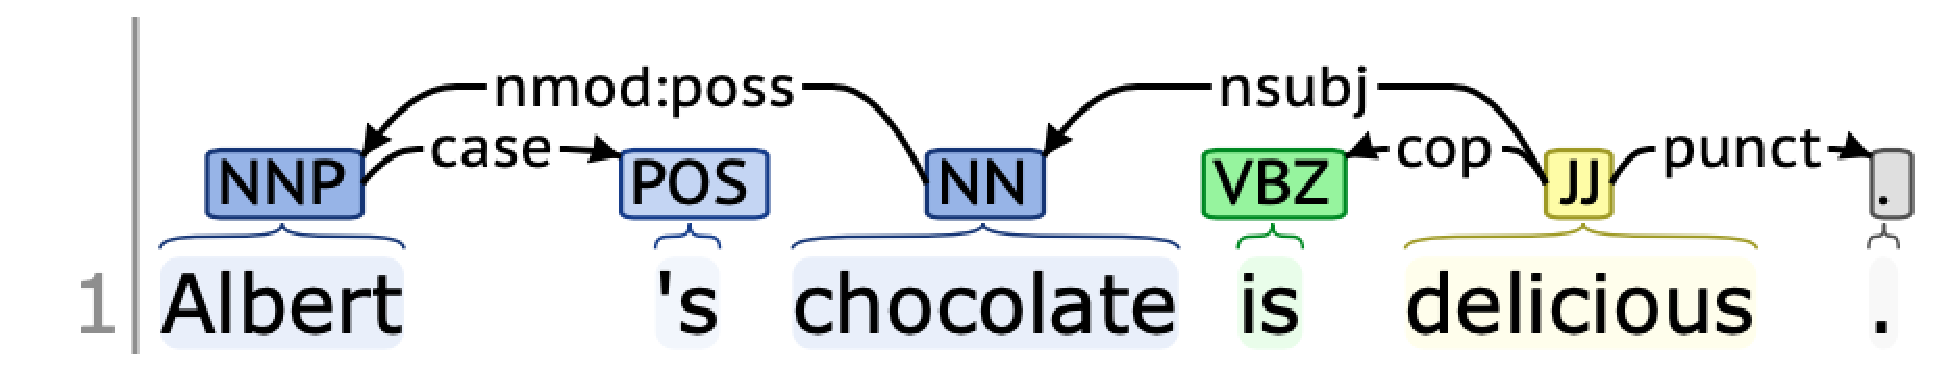
\includegraphics[width=0.75\textwidth]{basic_sentence_core_nlp.eps} \\ \midrule
\textbf{spaCy} & 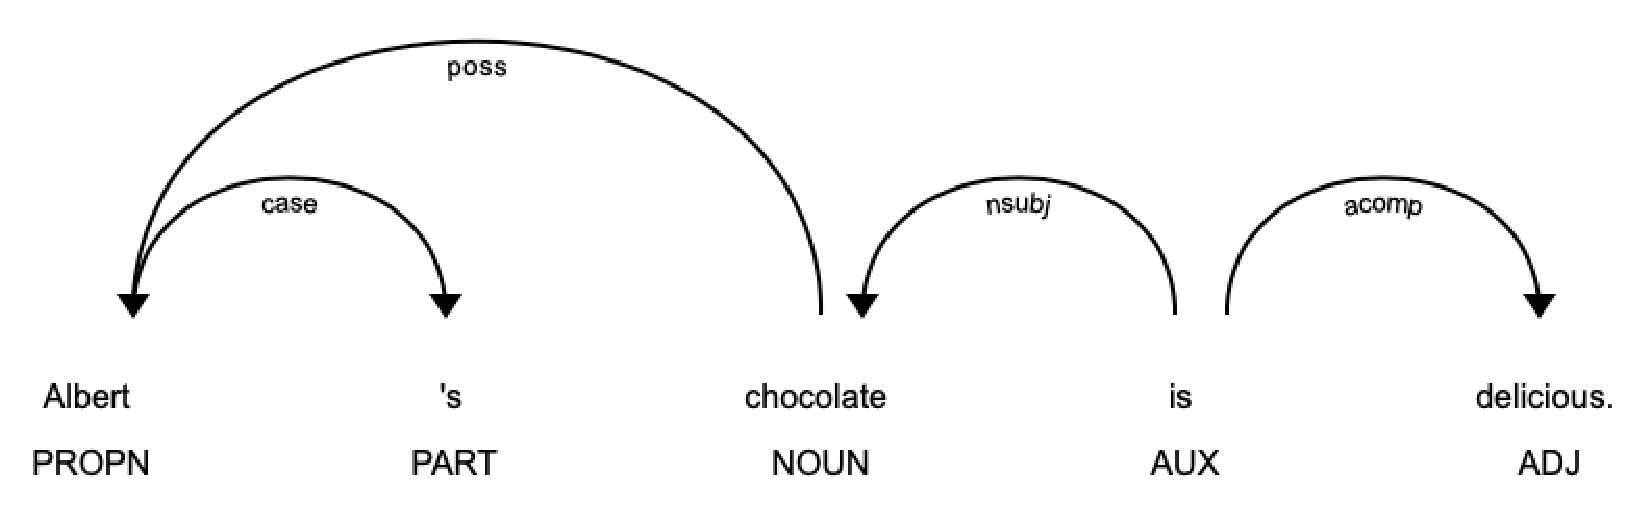
\includegraphics[width=0.85\textwidth]{basic_sentence_spacy.eps}  \\ \bottomrule
\end{tabular}
\caption{Semantic parsing example for a basic sentence}
\label{table:basic_sentence}
\end{table}

However, the English language can often be ambiguous and highly context-dependent, meaning that multiple \textit{parse trees} for the same sentence could emerge. Consider the following two sentences \cite{noauthor_studying_nodate}:
\begin{displayquote}
He fed her cat food. \\
I saw a man on a hill with a telescope.
\end{displayquote}
As shown in Table \ref{table:ambiguous_sentence}, both parsers interpret the meaning of the first example sentence as a person who feeds their ``cat food", which, in addition of not being very logical, is also grammatically incorrect as the genders do not match. Unfortunately, computers are generally not very good at context-based inference, something to take into account for this research project.

Therefore, accuracy is very important for \textit{syntactic parsing} \cite{gomez-rodriguez_how_2019}.

\begin{table}[H]
\centering
\begin{tabular}{@{}ll@{}}
\toprule
\textbf{CoreNLP} & 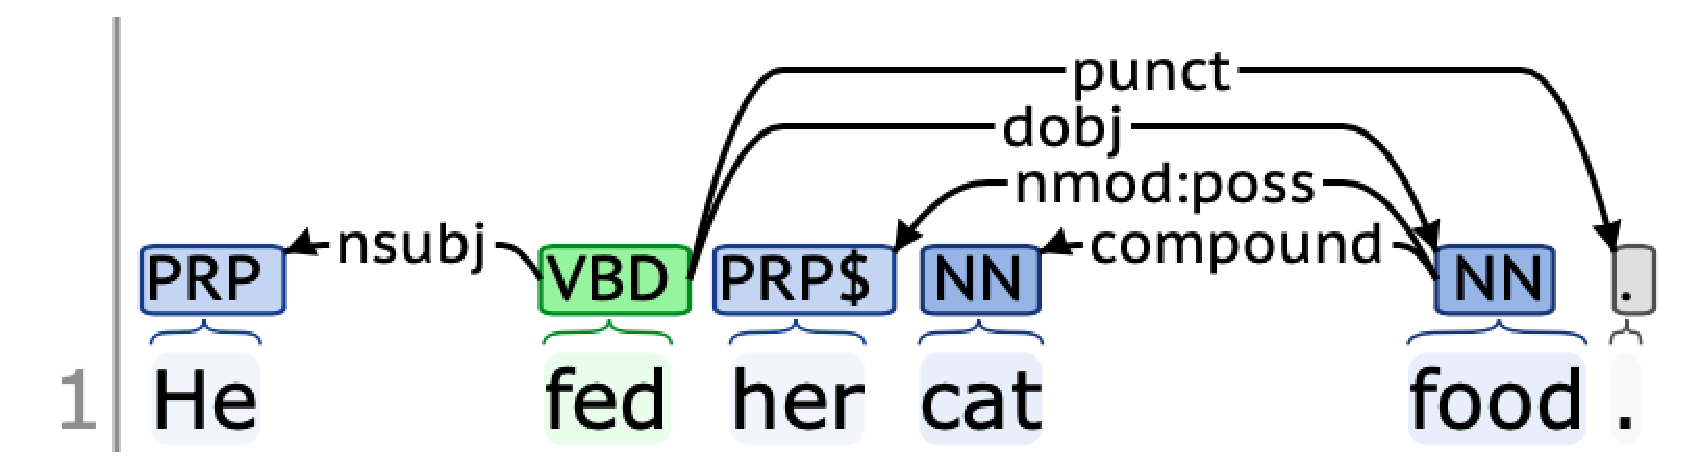
\includegraphics[width=0.75\textwidth]{ambiguous_sentence_core_nlp.eps} \\ \midrule
\textbf{spaCy} & 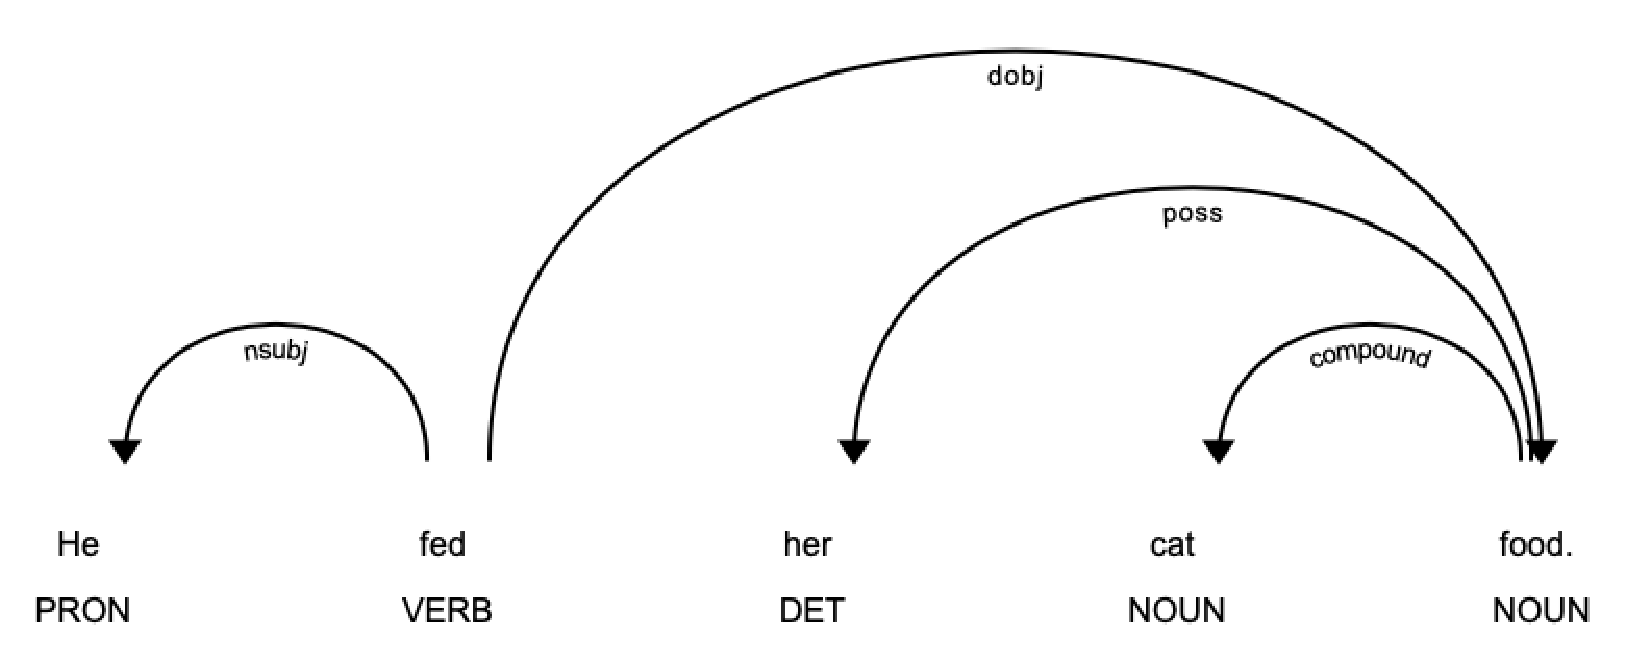
\includegraphics[width=0.85\textwidth]{ambiguous_sentence_spacy.eps}  \\ \bottomrule
\end{tabular}
\caption{Semantic parsing example for an ambiguous sentence}
\label{table:ambiguous_sentence}
\end{table}

\section{Logic Programming}
\label{sec:logic}

\begin{definition}[Term \cite{kowalski_predicate_1974}]
A \textit{term} is either a \textit{variable} $x,y,z,...$ or an expression $f(t_1,t_2,...,t_k)$, where $f$ is a k-ary \textit{function symbol} and the $t_i$ are \textit{terms}. A \textit{constant} is a 0-ary \textit{function symbol}.
\end{definition}

\begin{definition}[Atom \cite{kowalski_predicate_1974}]
An \textit{atomic formula} (or \textit{atom}) has the form $P(t_1,t_2,...,t_k)$, where $P$ is a k-ary predicate (boolean function) symbol and the $t_i$ are terms.
\end{definition}

\subsection{Answer Set Programming}

Once we have parsed a text, the next step is to convert this into an answer set program (ASP).

ASP is a declarative first-order (predicate) logic language whose aim is to solve complex search problems \cite{lifschitz_what_nodate}. It is built upon the idea of stable model (answer set) semantics, returns answer sets when asked for the solution to a problem.

In ASP, a \textit{literal} is an \textit{atom} \textit{a} or its negation \textit{not a} (we call this negation as a failure). ASP programs are composed of a set of \textit{normal rules}, whose head is a single \textit{atom} and body is a conjunction of \textit{literals} \cite{law_representing_2019}.
\begin{equation}
h \leftarrow b_1, b_2, ..., b_k, \text{not}\ b_{k+1}, ..., \text{not}\ b_m.
\end{equation}

If the body is empty ($k = m = 0$) then a rule is called a \textit{fact}. We can also have \textit{constraints}, which are like \textit{normal rules} except that the head is empty. These prevent any answer sets from both including $b_1, b_2, ..., b_k$ and excluding $b_{k+1}, ..., b_m$.

\begin{definition}[Safety \cite{law_representing_2019}]
A variable in a rule is said to be \textit{safe} if it occurs in at least one positive \textit{literal} (i.e., the $b_i$s in the above rule) in the body of the rule.
\end{definition}

\begin{definition}[Herbrand Base \cite{law_representing_2019}]
The \textit{Herbrand base} of a program P, denoted $HB_P$, is the set of variable-free (\textit{ground}) \textit{atoms} that can be formed from predicates and \textit{constants} in P. The subsets of $HB_P$ are called the (Herbrand) \textit{interpretations} of P.
\end{definition}

\begin{definition}[Satisfiability \cite{law_representing_2019}] 
\label{def:satisfiability}
Given a set $A$, a \textit{ground normal rule} of P is \textit{satisfied} if the head is in $A$ when all positive \textit{atoms} and none of the negated \textit{atoms} of the body are in $A$, that is when the body is \textit{satisfied}. A \textit{ground constraint} is \textit{satisfied} when the body is not \textit{satisfied}.
\end{definition}

\begin{definition}[Reduct \cite{law_representing_2019}]
Given a program P and a \textit{Herbrand interpretation} $I \subseteq HB_P$, the \textit{reduct} $P^I$ is constructed from the grounding of P in three steps:
\begin{enumerate}[nolistsep]
\item Remove rules whose bodies contain the negation of an atom in I.
\item Remove all negative \textit{literals} from the remaining rules.
\item Replace the head of any constraint with $\bot$ (where $\bot \notin HB_P$).
\end{enumerate}
For example, the \textit{reduct} of the program $\{a \leftarrow \text{not}\ b, c.\quad d \leftarrow \text{not}\ c.\}$ with respect to $I=\{b\}$ is $\{d.\}$.
\end{definition}

\begin{definition}[Minimal Model]
We say that $I$ is a (Herbrand) \textit{model} when $I$ \textit{satisfies} all the rules in the program P. It is a \textit{minimal model} if there exists no smaller \textit{model} than $I$.
\end{definition}

\begin{definition}[Answer Set \cite{law_representing_2019}]
Any $I \subseteq HB_P$ is an \textit{answer set} of P if it is equal to the \textit{minimal model}  of the \textit{reduct} $P^I$. We will denote the set of \textit{answer sets} of a program P with $AS(P)$. 
\end{definition}

\subsection{Context-Free Grammars}

In order to discuss ASGs, we must first define \textit{context-free grammars} (CFGs) and \textit{parse trees}. An example for these is shown in Figure \ref{fig:cfg_parse_tree_example}.

\begin{definition}[Context-Free Grammar \cite{scheinberg_note_1960}]
A CFG is a finite set G of ``rewriting rules" $\alpha \to \beta$, where $\alpha$ is a single symbol and $\beta$ is a finite string of symbols from a finite alphabet (vocabulary) V. V contains precisely the symbols appearing in these rules plus the ``boundary" symbol $\epsilon$, which does not appear in these rules. Rules of the form $\alpha \to \alpha$ (which have no effect) are not allowed.
\end{definition}

\begin{definition}[Parse Tree \cite{law_representing_2019}]
Let $GCF$ be a CFG. A \textit{parse tree} $PT$ of $GCF$ for a given string consists of a node $node(PT)$, a list of \textit{parse trees}, called \textit{children} and denoted $children(PT)$, and a rule $rule(PT)$, such that:
\begin{enumerate}[nolistsep]
\item If $node(PT)$ is a terminal node, then $children(PT)$ is empty.
\item If $node(PT)$ is non-terminal, then $rule(PT)$ is of the form $node(PT) \to n_1 ... n_k$ where each $n_i$ is equal to $node(children(PT)[i])$ and $|children(PT)| = k$.
\end{enumerate}
\end{definition}

\begin{definition}[Trace \cite{law_representing_2019}]
We can represent each node n in a \textit{parse tree} by its \textit{trace}, $trace(n)$, through the tree. The \textit{trace} of the root is the empty list \texttt{[]}; the i\textsuperscript{th} child of the root is \texttt{[i]}; the j\textsuperscript{th} child of the i\textsuperscript{th} child of the root is \texttt{[i, j]}, and so on.
\end{definition}

\begin{figure}[H]
\begin{subfigure}{0.3\textwidth}
\texttt{1: start -> as "b" \\ 2: as -> "a" as \\ 3: as ->\\}
\caption{CFG for \texttt{a\textsuperscript{i}b}}
\end{subfigure}
\begin{subfigure}{0.34\textwidth}
\begin{table}[H]
\centering
\begin{tabular}{@{}ccc@{}}
\toprule
\textbf{$trace(n)$} & \textbf{$node(n)$} \\ \midrule
\texttt{[]} & \texttt{start} \\
\texttt{[1]} & \texttt{as} \\
\texttt{[1,1]} & \texttt{a} \\
\texttt{[1,2]} & \texttt{as} \\
\texttt{[1,2,1]} & \texttt{a} \\
\texttt{[1,2,2]} & \texttt{as} \\
\texttt{[2]} & \texttt{b} \\ \bottomrule
\end{tabular}
\end{table}
\caption{\textit{Parse tree} table for \texttt{aab}}
\end{subfigure}
\begin{subfigure}{0.34\textwidth}
\centering
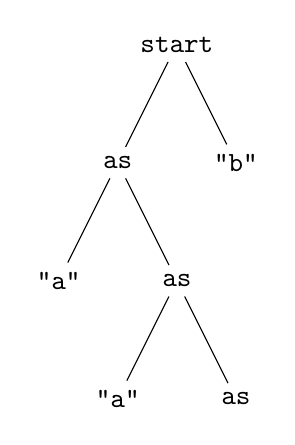
\begin{tikzpicture}
\node {\texttt{start}}
  child {node {\texttt{as}}
    child {node {\texttt{"a"}}}
    child {node {\texttt{as}}
      child {node {\texttt{"a"}}}
      child {node {\texttt{as}}}}}
  child {node {\texttt{"b"}}};
\end{tikzpicture}
\caption{\textit{Parse tree} graph for \texttt{aab}}
\end{subfigure}
\caption{Example of a CFG and its \textit{parse tree}}
\label{fig:cfg_parse_tree_example}
\end{figure}

\subsection{Answer Set Grammars}

ASGs are an extension of CFGs, whereby each production rule is \textit{annotated}. More specifically, $P$ can be a \textit{ground term}, such as in the \textit{annotated atom} \texttt{a(1)@2} (referring to the second child of this node). The example shown in Figure \ref{fig:asg_example} is a subset of the language \texttt{a\textsuperscript{i}b} captured by the CFG in Figure \ref{fig:cfg_parse_tree_example},  restricting it to the language \texttt{a\textsuperscript{n}} where $\texttt{n} \ge 2$ (the string contains at least two as).

\begin{definition}[Answer Set Grammar \cite{law_representing_2019}]
 An \textit{annotated} production rule is of the form $n_0 \to n_1 ... n_k\ P$ where $n_0 \to n_1 ... n_k$ is an ordinary CFG production rule and $P$ is an \textit{annotated} ASP program, where every \textit{annotation} is an integer from $1$ to $k$.
\end{definition}

\begin{figure}[H]
\texttt{1: start -> as "b" \{ :- size(X)@1, X < 1. \} \\
           2: as -> "a" as \space\space\space\{ size(X+1) :- size(X)@2. \} \\
           3: as -> \space\space\space\space\space\space\space\space\space\space\{ size(0). \} \\}\\
* Intuitively, \texttt{size} represents the length of the current string.
\caption{Example of an ASG}
\label{fig:asg_example}
\end{figure}

\begin{definition}[Parse Tree Program \cite{law_representing_2019}]
Let G be an ASG and PT be a \textit{parse tree}. $G[PT]$ is the program $\{\ rule(n)@trace(n)\ |\ n \in PT\ \}$, where for any production rule $n_0 \to n_1...n_k\ P$, and any trace $t$, $PR@t$ is the program constructed by replacing all annotated atoms $a@i$ with the atom $a@t++[i]$ and all \textit{unannotated atoms} $a$ with the atom $a@t$.
\end{definition}

\begin{definition}[Conforming Parse Tree \cite{law_representing_2019}]
Given a string $str$ of terminal nodes, we say that $str \in \mathcal{L}(G)$ ($str$ \textit{conforms} to the language of G) if and only if there exists a parse tree PT of G for $str$ such that the program $G[PT]$ is \textit{satisfiable}. For such a PT, every single rule in the language must be satisfied (see Definition \ref{def:satisfiability}).
\end{definition}

As shown in Figure \ref{fig:asg_tree_program_example}, $\texttt{aab} \in \mathcal{L}(G)$, and the corresponding program has a single answer set $\{size(0)@[1,2,2],\ size(1)@[1,2],\ size(2)@[1]\}$. From this example, it is easy to see how the corresponding program would be \textit{unsatisfiable} for the string \texttt{ab}.

\begin{figure}[H]
\centering
\texttt{:- size(X)@[1], X < 1. \\
           size(X+1)@[1] :- size(X)@[1,2]. \\
           size(X+1)@[1,2] :- size(X)@[1,2,2]. \\
           size(0)@[1,2,2].}
\caption{$G[PT]$ for the \textit{parse tree} and ASG from the examples above}
\label{fig:asg_tree_program_example}
\end{figure}

\subsection{Learning Answer Set Grammars}

Given an incomplete ASG, it is possible to learn the complete grammar by induction (which uses \textbf{ILASP}\footnote{ILASP is a logic-based machine learning system: \url{http://www.ilasp.com}}), as long as we provide some \textit{positive examples} (strings which should conform to the language) and/or \textit{negative examples}  (strings which must not), as well as a \textit{hypothesis space} and usually some \textit{background} information. Note that the \textit{background} is only used for ``global" knowledge, such as defining what is a number, or how to increment one \cite{law_representing_2019}.

In such an \textit{inductive learning program} (ILP) task, we have a \textit{hypothesis space} in the form of \textit{mode declarations}, defining the format of the heads (written \texttt{\#modeh}) and bodies (written \texttt{\#modeb}) of rules which can be learned. It is also possible to restrict the scope of a particular \textit{mode declaration} by specifying a list of rule numbers at the end. Note that there are two forms of body \textit{mode declarations}: \texttt{\#modeba} is used for predicates that accept an $@$ \textit{annotation}, and \texttt{\#modebb} is intended for those without (which are defined in \texttt{\#background}). An example is shown in Figure \ref{fig:asg_ilp_example}.

\begin{figure}[H]
\centering
\begin{subfigure}{0.55\textwidth}
\texttt{start -> as bs \{\} \\
as -> "a" as \{\} | \{\} \\
bs -> "b" bs \{\} | \{\} \\
\newline
+ [] \\
+ ["a", "b"] \\
+ ["a", "a", "b", "b"] \\
- ["a"] \\
- ["b"] \\
- ["a", "a"] \\
- ["b", "b"] \\
- ["a", "a", "b"] \\
- ["a", "b", "b"] \\
\newline
\#background \{ \\
num(0). num(1). num(2). num(3). \\
inc(X,X+1) :- num(X), num(X+1). \} \\
\newline
\#modeh(size(var(num))):[2,3,4,5]. \\
\#modeh(size(0)):[2,3,4,5]. \\
\#modeba(size(var(num))). \\}
\caption{Input incomplete program}
\end{subfigure}
\begin{subfigure}{0.44\textwidth}
\texttt{start -> as bs \{ \\
\phantom{ }:- not size(X)@2, size(X)@1. \\
\} \\
\newline
as -> "a" as \{ \\
\phantom{ }size(X+1) :- size(X)@2. \\
\} \\
\newline
as -> \{ \\
\phantom{ }size(0). \\
\} \\
\newline
bs -> "b" bs \{ \\
\phantom{ }size(X+1) :- size(X)@2. \\
\} \\
\newline
bs -> \{ \\
\phantom{ }size(0). \\
\}} \\
\caption{Output learned program}
\end{subfigure}
\newline
\newline
* Note: the symbol \texttt{|} indicates multiplicity of production rules.
\caption{Example of an ASG ILP task for the language \texttt{a\textsuperscript{n}b\textsuperscript{n}}}
\label{fig:asg_ilp_example}
\end{figure}

\section{Neural Networks}
\label{sec:neural_networks}

\subsection{Recurrent Neural Networks}

A recurrent neural network (RNN) is a chain-like neural network that is applied once for each \textit{token} in the input sequence. At each timestep $t$ in a ``vanilla" RNN (i.e., for each item in the sequence), the current \textit{hidden state} $h_t$ is computed as a function of the previous \textit{hidden state} $h_{t-1}$ and the current input \textit{token} $x_t$, using a non-linear \textit{activation function} (usually sigmoid) \cite{cho_learning_2014}.

\subsection{Long Short-Term Memories}

A long short-term memory (LSTM) is a particular kind of RNN, motivated by the problems of vanishing and exploding gradients which sometimes occur due to the chain-like nature of RNNs. The solution here is to at each timestep use what is called a \textit{memory block}, which holds at it center a linear unit that is connected to itself. In addition, it has three \textit{gates}: input ($i$), forget ($f$) and output ($o$). Respectively, these three \textit{gates} are concerned with which information to store, how long to store it, and when it should be passed on \cite{gers_learning_2000}.

Finally, each \textit{memory block} also stores a \textit{cell state} $c_t$, which combines information from the previous \textit{cell state} $c_{t-1}$ and from the \textit{candidate state} $g_t$ (defined as per the \textit{hidden state} in a vanilla RNN), using the \textit{forget} and \textit{input} \textit{gates} to regulate information flow. The \textit{hidden state} $h_t$ is then defined as a function of this \textit{cell state}, controlled by the \textit{output gate}. Figure \ref{fig:memory_block} shows this diagrammatically \cite{graves_hybrid_2013}.

\begin{equation}
\begin{aligned}
i_t &= \sigma(W_{xi} \cdot x_t + W_{hi} \cdot h_{t-1} + W_{ci} \cdot c_{t-1} + b_i) \\
f_t &= \sigma(W_{xf} \cdot x_t + W_{hf} \cdot h_{t-1} + W_{cf} \cdot c_{t-1} + b_f) \\
o_t &= \sigma(W_{xo} \cdot x_t + W_{ho} \cdot h_{t-1} + W_{co} \cdot c_t + b_o) \\
g_t &= tanh(W_{xg} \cdot x_t + W_{hg} \cdot h_{t-1} + b_g) \\
c_t &= f_t \cdot c_{t-1} + i_t \cdot g_t \\
h_t &= tanh(c_t)
\end{aligned}
\end{equation}

\begin{figure}[H]
\centering
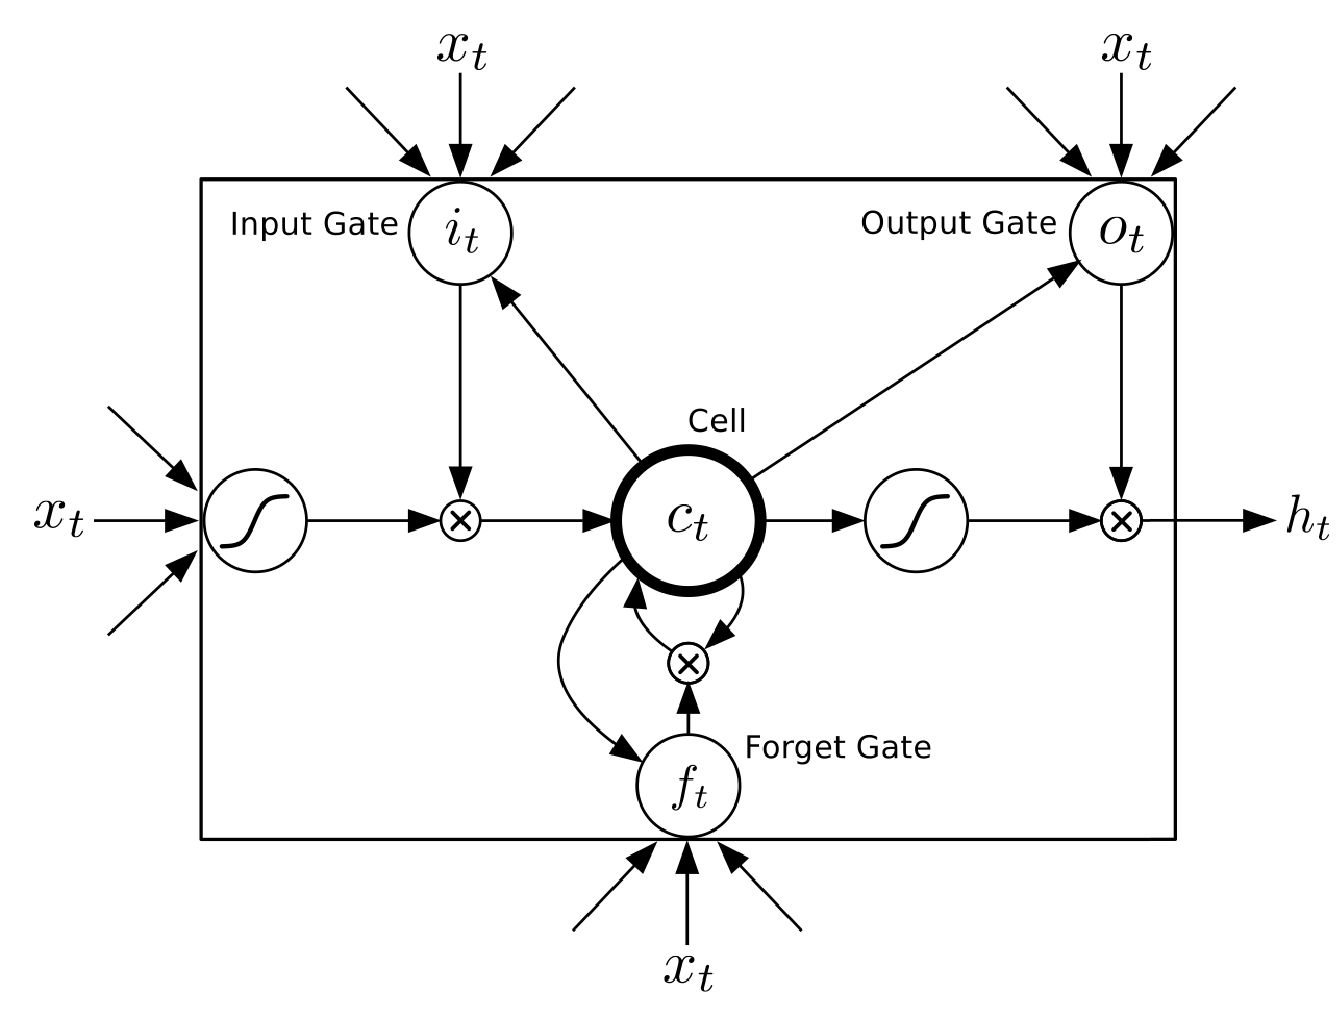
\includegraphics[width=0.62\textwidth]{memory_block.eps}
\caption{\cite{graves_hybrid_2013} Diagram showing the flow of information in an LSTM \textit{memory block}}
\label{fig:memory_block}
\end{figure}

\subsection{Encoder-Decoders}

An \textit{encoder-decoder} is a neural network consisting of two eponymous RNNs, are often LSTMs. The \textit{encoder}'s job is to translate any variable-length sequence given as input into a fixed-length vector representation, while the \textit{decoder}'s role is to transform this into a new variable-length sequence. Together, they are trained to maximize the probability of generating a target sequence given the corresponding input sequence \cite{cho_learning_2014}.

\subsection{Attention}

In the context of neural machine translation (NMT) systems such as \textit{encoder-decoders}, the driver behind \textit{attention} is to improve performance by selectively looking at sub-portions of the input sequence, which becomes especially important for long sequences of text \cite{yao_dual_2018}.

\subsubsection{Global Attention}

On top of being dependant on the last \textit{hidden state} $d_{t-1}$ and output \textit{token} $y_{i-1}$, every \textit{hidden state} $d_t$ in a \textit{decoder} with \textit{global attention} is computed also in function of its \textit{context vector} $c_t$. Each \textit{context vector} $c_t$ is defined as a weighted sum of the \textit{encoder}'s \textit{hidden states} $h_i$. The $h_i$ that are assigned a higher weight are that which are more similar to $d_t$, which is done using a trainable \textit{alignment model} $a$ \cite{bahdanau_neural_2016}.

\begin{equation}
\begin{aligned}
c_t &= \sum_{i} \alpha_{ti} \cdot h_t \\
\mbox{where } \alpha_{ti} &= \frac{exp(s_{ti})}{\sum_{j} exp(s_{tj})} \\
s_{ti} &= a(d_{t-1},h_i)
\end{aligned}
\end{equation}

Here the idea is that $\alpha_{ti}$ tells us how important each $h_i$ is with respect to the current timestep $t$, influencing the value of $d_t$ and hence the decision of the generated output \textit{token} $y_t$. Essentially, this is a way of telling the \textit{decoder} which parts of the input sequence to pay attention to. Thanks to this mechanism, the \textit{encoder} is no longer forced to compress all the useful information from an input sequence into a fixed-length vector, thus improving performance for longer sequences of \textit{tokens} \cite{bahdanau_neural_2016}.

\chapter{Preprocessor}
\label{chapter:preprocessor}

\section{Overview}

In order to prepare the story to be parsed and summarized by \textsc{SumASG}, we have created the \textsc{Preprocessor}. As we will loose information in summary anyway, it is completely acceptable to... which steps are shown below in Figure \ref{fig:preprocessor_pipeline}.

\begin{figure}[H]
\centering

\begin{tikzpicture}[node distance=0.45cm, auto]
\node (story_in) [] {Story};
\node (tokenize) [block, right =of story_in] {Tokenize};
\node (simplify) [block, right =of tokenize] {Simplify};
\node (prune) [block, right =of simplify] {Prune};
\node (homogenise) [block, right =of prune] {Homogenise};
\node (story_out) [block, right =of homogenise] {Preprocessed Story};
\draw [->] (story_in) -- (tokenize);
\draw [->] (tokenize) -- (simplify);
\draw [->] (simplify) -- (prune);
\draw [->] (prune) -- (homogenise);
\draw [->] (homogenise) -- (story_out);
\end{tikzpicture}
\caption{Preprocessor Steps}
\label{fig:preprocessor_pipeline}
\end{figure}

\section{Tokenization And Simplification}
\label{sec:tokenization_scoring}

With the help of \textbf{CoreNLP}, we can assign a POS tag to each word, or \textit{token}, from the input story. Using this information, we can now make a number of simplifications which will make the sentence structure more consistent throughout.

\subsection{Punctuation}
\label{subsec:punctuation}

To avoid having to build recognition and semantic understanding of different types of punctuation into \textsc{SumASG}, it is preferable to transform the story such that it uses no punctuation apart from full stops. The idea is that each sentence in the resulting text contains exactly one action or description.

Depending on the type of punctuation used at the end of a clause, a different treatment is applied:
\begin{itemize}[nolistsep]
\item Question marks: We remove the clause, as it is most likely irrelevant for this task. It also helps avoid negation since we are deleting rhetorical questions.
\item Dashes: These are used around clauses which add detail, so it is quite safe to delete them for the task of summarization.
\item Exclamation marks, commas, semi-colons and colons: We replace any of these with a full stop.
\end{itemize}

\subsection{Individual Word Transformations}

One of the main goals of the \textsc{Preprocessor} is to transform the story in a simple and consistent structure, one where a given POS tag may only appear in a limited number of places in a sentence.

\subsubsection{Acronyms}

Some acronyms are often spelled using full stops after each letter. To prevent these from being recognized as multiple sentences, it is beneficial to remove any punctuation from acronyms. Therefore the word ``U.S.A." would become ``USA".

\subsubsection{Contractions}

Contractions can be difficult to understand for machines, and they add unwanted complexity to the task of parsing. Therefore it is simplest to expand all of them, for example transforming ``it's" into ``it is".

\subsubsection{Adverbs}

In the English language, adverbs can appear almost anywhere in a sentence, and their position has minimal semantic influence. To illustrate this, consider the following sentences, which all have the same meaning:

\begin{displayquote}
\underline{Slowly} he eats toast. \\
He \underline{slowly} eats toast. \\
He eats toast \underline{slowly}.
\end{displayquote}

In order to provide \textsc{SumASG} with a consistent format for parsing adverbs, we should always move them to the end of the clause in which they appear (in the above example we would keep the last sentence).


\subsubsection{Determiners}

In the English language, the determiners ``a" and ``an" are semantically identical, so to makes sense to only use one of the two, with the intention of reducing the number of \textit{tokens} that \textsc{SumASG has to process}. We can always correct the output of \textsc{SumASG} to make it grammatically-correct.

\subsubsection{Possessive Pronouns, Interjections And Prepositions}

In most cases, possessive pronouns and interjections do not add much to the meaning of a story, especially when the end goal is to create a summary. Therefore, we can remove such words from the text. For instance, the sequence ``\underline{Ah}! She ate \underline{her} chocolate." would become ``She ate chocolate.".

Prepositions which appear at the start of a sentence may be removed, as they are not integral to the meaning. For example, ``\underline{Besides} today is Sunday" gets transformed into ``Today is Sunday".

Moreover, prepositions which come after the object in a sentence can sometimes cause it to become syntactically too complex. Rather than encoding such high-level of detail into the internal representation of \textsc{SumASG}, it is preferable to simply omit the final clause. In this case, ``They have a picnic \underline{under} a tree." becomes ``They have a picnic.". Although some information is thrown away, this loss will usually have no impact on the quality of the summary.

\subsection{Clause Transformations}

After going through the \textsc{Preprocessor}, we would like each sentence in the given story to only focus on a single topic.

When possible, we should split sentences containing multiple clauses into individual sentences. Otherwise, we can delete the auxiliary clause and keep the main clause.

Examples of the transformations applied to different types of clauses can be seen below in Figure \ref{fig:clause_transformations}.

\begin{figure}[H]
\begin{subfigure}{\textwidth}
\begin{displayquote}
\textit{Conjunctive Clause} We looked left \underline{and} they saw us.\\
\textit{Conjunctive Clause}. Cars have wheels \underline{and} go fast.\\
\textit{Subordinating Clause}. She never walks alone \underline{because} she is afraid.\\
\textit{Dependant Clause}. I want to be President \underline{when I grow up}.\\
\textit{Dependant Clause}. \underline{When I grow up}, I will have a garden.
\end{displayquote}
\caption{Before transformation}
\vspace{\baselineskip}
\end{subfigure}
\begin{subfigure}{\textwidth}
\begin{displayquote}
\textit{Conjunctive Clause}. We looked left. they saw us.\\
\textit{Conjunctive Clause}. Cars have wheels. Cars go fast.\\
\textit{Subordinating Clause}. She never walks alone. she is afraid.\\
\textit{Dependant Clause}. I want to be President.\\
\textit{Dependant Clause}. I will have a garden.
\caption{After transformation}
\end{displayquote}
\end{subfigure}
\caption{Examples of the splitting of multi-clause sentences}
\label{fig:clause_transformations}
\end{figure}

\subsubsection{Hypernym Substitution}

However, in some cases we may be able to perform an optimization that allows us to collapse a conjunction of two words into a common \textit{hypernym} (i.e. superclass).

In practice, this involves using \textbf{\href{http://web.archive.org/web/20190516161631/https://www.clips.uantwerpen.be/pages/pattern-en}{Pattern}} to try and find a lexical field to which both words pertain.

For example, the words ``chicken" and ``goose" both belong to the lexical field of ``poultry". Similarly, ``cars" and ``trucks" have common hypernym ``motor-vehicles".

\textcolor{red}{\textbf{\hl{TODO give more details about how chosen?}}}

\subsection{Case And Proper Nouns}

We want to ensure that all occurrences of a word are treated as the same \textit{token}. Since \textsc{SumASG} will be generating new sentences from scratch, the simplest solution is to convert the entire story to lower-case, apart from proper nouns.

In the case of complex proper nouns (i.e., those constructed from multiple words), we should remove inner spaces so that we end up with a camel-case string. For instance, the sequence ``Peter Little" will become ``PeterLittle".

We can also do this with complex common nouns, for example transforming ``bird house" into ``bird-house".

\subsubsection{Pronoun Substitution}

Sometimes, an author will introduce a character or group by name, and later refer to them using a pronoun.

If a story contains exactly one distinct singular proper noun and then uses either ``he" or ``she", then it is safe to assume that this pronoun refers the aforementioned proper noun. The same can be said about plural proper nouns and the pronoun ``they".
To clarify this, an example is shown in Figure \ref{fig:pronoun_substitution}.

\begin{figure}[H]
\begin{subfigure}{\textwidth}
\begin{displayquote}
\textbf{Antonio} is a cheesemaker. \underline{He} makes burrata.
\textbf{Italians} eat pasta. \underline{They} make it with egg sometimes.
\end{displayquote}
\caption{Before transformation}
\vspace{\baselineskip}
\end{subfigure}
\begin{subfigure}{\textwidth}
\begin{displayquote}
\textbf{Antonio} is a cheesemaker. \textbf{Antonio} makes burrata.
\textbf{Italians} eat pasta. \textbf{Italians} make it with egg sometimes.
\caption{After transformation}
\end{displayquote}
\end{subfigure}
\caption{Example of substituting pronouns with proper nouns}
\label{fig:pronoun_substitution}
\end{figure}

\subsection{Example}
\label{subsec:simplification_example}

The result of running the simplification transformations is illustrated below in Figure \ref{fig:simplification_example}. Please refer to Chapter \ref{chapter:contributions} for the original story.

\begin{figure}[H]
\begin{subfigure}{\textwidth}
\begin{displayquote}
\begin{enumerate}[label=\protect\circled{\alph*}]
\item Adverbs: move ``always" and ``Now" to the end of the sentence
\item Determiners: ``an" $\rightarrow$ ``a"
\item Possessive pronouns: \st{``his"}
\item Prepositions: \st{``So"}
\item Conjunctive clauses: ``serious in school" $\|$ ``did homework always"
\item Dependant clauses: \st{``When he was older"}
\item Complex clauses: ``was a curious little boy" $\|$ ``named Peter Little"
\item Hypernym substitution: ``stars and planets" $\rightarrow$ ``astronomy"
\item Case: make all words but proper nouns lower case
\item Complex nouns: ``Peter Little" $\rightarrow$ ``PeterLittle"
\item Complex nouns: ``quantum physics" $\rightarrow$ ``quantum-physics"
\item Pronoun substitution: ``he" $\rightarrow$ ``PeterLittle"
\end{enumerate}
\end{displayquote}
\caption{Transformations applied (where $\|$ means splitting into multiple sentences)}
\vspace{\baselineskip}
\end{subfigure}
\begin{subfigure}{\textwidth}
\begin{displayquote}
\textbf{0.} there was a curious little boy.\\
\textbf{1.} \circled{g} the curious little boy was named \circled{j} PeterLittle.\\
\textbf{2.} \circled{l} PeterLittle was interested in \circled{h} astronomy.\\
\textbf{3.} \circled{d} PeterLittle was serious in school.\\
\textbf{4.} \circled{e} PeterLittle did \circled{c} homework \circled{a} always.\\
\textbf{5.} \circled{f} PeterLittle studied mathematics and \circled{k} quantum-physics.\\
\textbf{6.} PeterLittle studied for \circled{c} exams hard.\\
\textbf{7.} PeterLittle became \circled{b} a astrophysicist.\\
\textbf{8.} PeterLittle is famous \circled{a} now.
\caption{Sentences after applying transformations}
\end{displayquote}
\end{subfigure}
\caption{Example of applying \textit{simplification} to the story of Peter Little}
\label{fig:simplification_example}
\end{figure}

\section{Sentence Pruning And Homogenization}

Once the sentence structure of the story has been \textit{simplified}, one of the main jobs of the \textsc{Preprocessor} is to remove irrelevant semantic complexity from the story.

In order to understand what is relevant in a story and what is not, the \textsc{Preprocessor} looks at the semantic similarity between words with the same POS tag (or a related one, i.e. singular noun and plural noun, or verbs with a different tense).

\subsection{Word Similarity}

It uses a loop to iterate over each sentence, and compares each word with every word from other sentences which have the same or a related POS tag. For each comparison, word \textit{similarity} is computed using the tool \href{http://www.conceptnet.io}{ConceptNet}, a semantic knowledge network.

As you might imagine, having such nesting of loops can be quite expensive, which is why we keep a cache of previously requested similarities, and use the fact that this \textit{similarity} relation is symmetric.

\subsection{Sentence Similarity And Pruning}

\subsubsection{Sentence Similarity}

Once we have computed the \textit{similarity} between words of different sentences, we can add these up on a per-sentence basis, which gives us a binary relation of \textit{similarity} between sentences.

We now have enough information to generate a \textit{text relationship map} over the sentences. The idea is that the more ``linked" a sentence is, the more relevant it is to the story. For each sentence, we therefore take the sum of the values of all its \textit{similarity} relations with other sentences. The higher this number, the more relevant, or \textit{important}, the sentence is to the story.

\subsubsection{Pruning}

In the interest of removing irrelevant sentences to help \textsc{SumASG}, we compute the 25th percentile over the \textit{importances} of all the sentences. We then prune sentences whose \textit{importance} is strictly less than this value.

In most cases, one quarter of the story will be pruned. However, if every sentence has the same \textit{importance}, then nothing gets removed. On the other hand, if two thirds of the story are very \textit{important} and the rest is irrelevant, then we remove more than a quarter of the sentences.

\subsection{Synonyms And Homogenization}

Another use for \textit{word similarity} is to find out if the author of the story has used any synonyms. When the \textit{similarity} between two words is above a certain threshold, then we consider them to be synonyms.

For every set of synonyms we find, we can choose a unique \textit{representative} for the set, and replace occurrences of the other words in that set with our \textit{representative}. For simplicity, we choose the \textit{representative} as the shortest word in its synonym set.

This is what we call \textit{story homogenization}, and it helps \textsc{SumASG} link words that would otherwise be considered completely different \textit{tokens} in the story.

\subsection{Example}

An example is shown below in Figure \ref{fig:preprocessor_example} for the story of Peter Little, where the weight between two nodes denotes \textit{similarity}. In this example, we consider words to be synonyms whenever their \textit{similarity} is at least 20. The labels of the nodes (starting from 0) for sentence \textit{similarity} correspond to the index of the sentence in the \textit{simplified story} (see Subsection \ref{subsec:simplification_example}).

As you can see, sentences 5 and 6 are deemed irrelevant and will be pruned, while sentences 0, 1 and 2 are thought as being very important.

Moreover, {homework, school} and {interested, curious} are considered synonym sets, and \textit{homogenization} will replace occurrences of these words with their shortest synonym (which may be itself).

\begin{figure}[H]
\begin{subfigure}{\textwidth}
\begin{subfigure}{0.5\textwidth}
\renewcommand\thesubfigure{\roman{subfigure}}
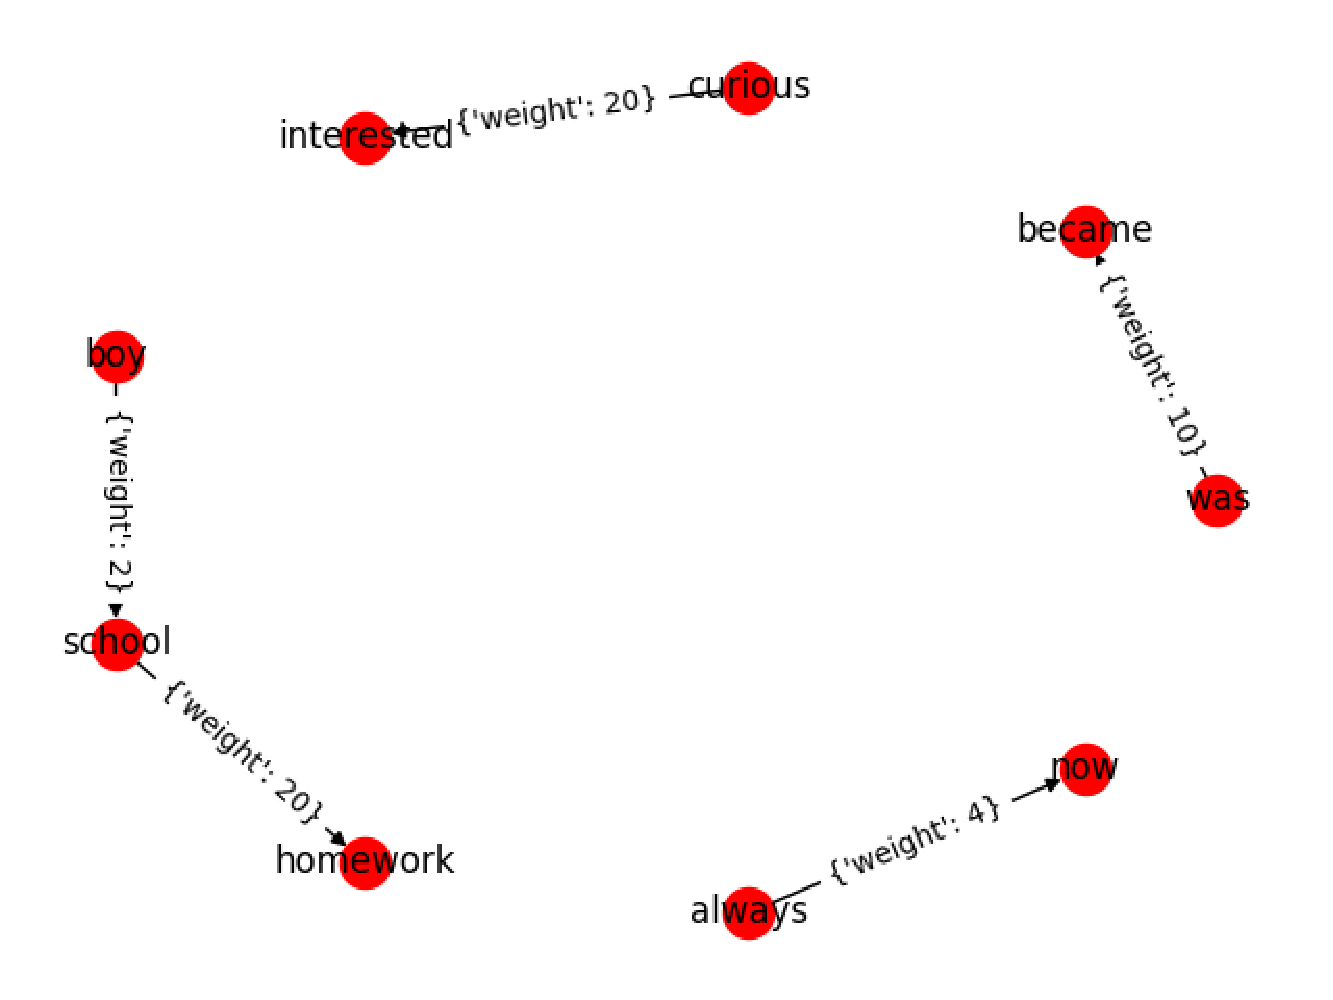
\includegraphics[width=\textwidth]{word_similarity.eps}
\caption{Word \textit{similarity}}
\end{subfigure}
\begin{subfigure}{0.5\textwidth}
\renewcommand\thesubfigure{\roman{subfigure}}
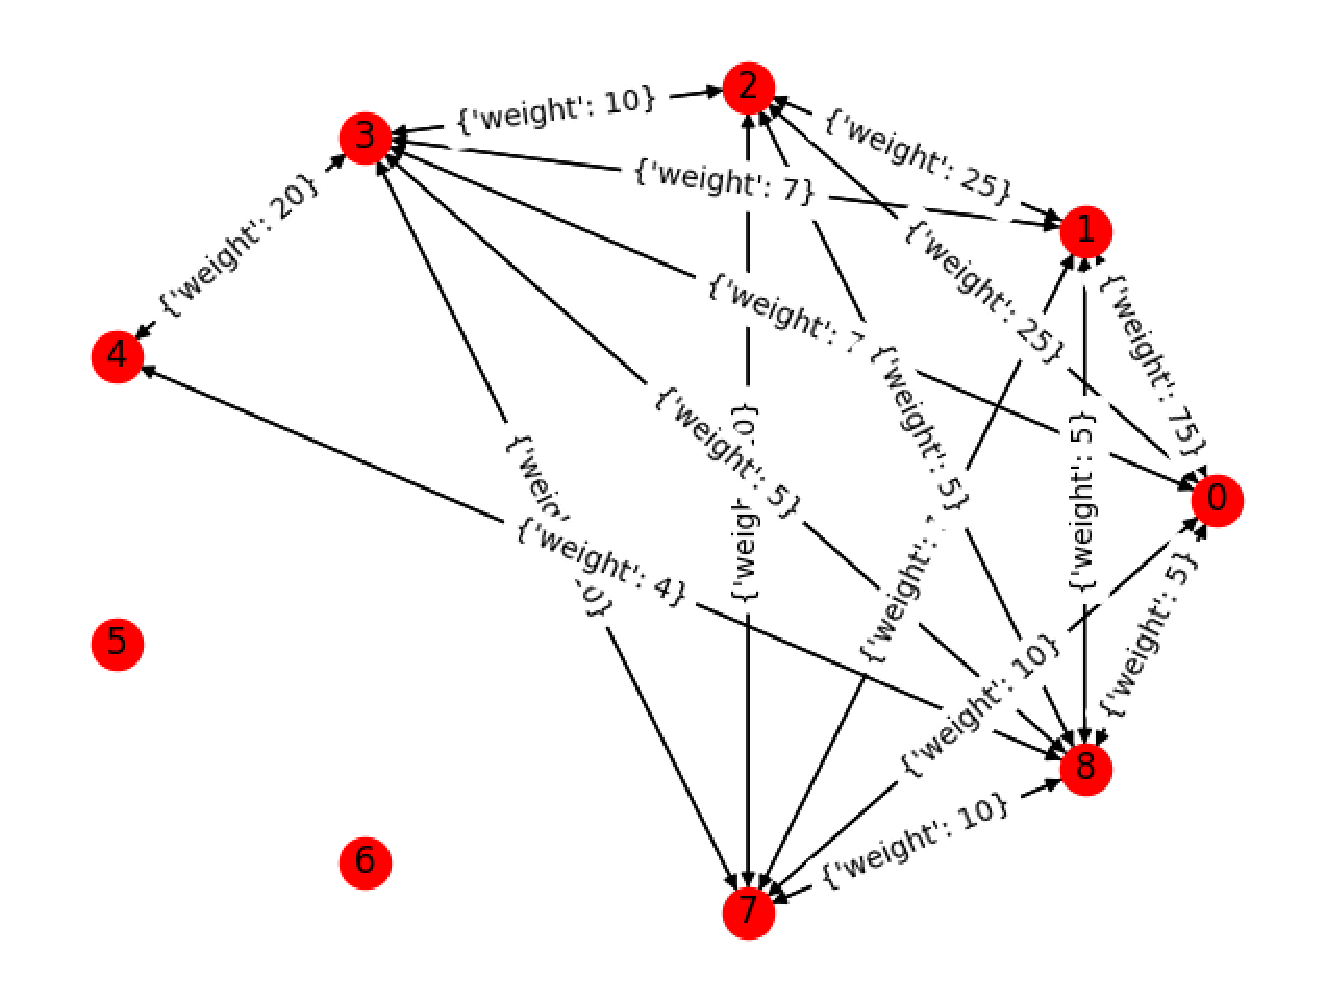
\includegraphics[width=\textwidth]{sentence_similarity.eps}
\caption{Sentence \textit{similarity}}
\end{subfigure}
\setcounter{subfigure}{0}
\caption{\textit{Text relationship maps}}
\end{subfigure}
\begin{subfigure}{\textwidth}
\vspace{\baselineskip}
\centering
\begin{tabular}{@{}llllllllll@{}}
\toprule
Sentence   & 0    & 1    & 2    & 3    & 7    & 8    & 4 & 5 & 6 \\ \midrule
Importance & 40.7 & 24.4 & 18.8 & 14.8 & 12.5 & 11.3 & 6 & 0 & 0 \\ \bottomrule
\end{tabular}
\caption{Sentences ordered by importance}
\end{subfigure}
\begin{subfigure}{\textwidth}
\vspace{\baselineskip}
\begin{displayquote}
there was a curious little boy. the curious little boy was named PeterLittle. PeterLittle was curious in astronomy. PeterLittle was serious in school. PeterLittle did school always. PeterLittle became a astrophysicist. PeterLittle is famous now.
\end{displayquote}
\caption{\textit{Homogenized} story}
\end{subfigure}
\caption{Example of applying sentence pruning and \textit{homogenization} to the \textit{simplified} story of Peter Little}
\label{fig:preprocessor_example}
\end{figure}

\section{Expandability}

In its current state, \textsc{SumASG} expects positive sentences only, and the only form of punctuation recognized is the full stop.

\subsection{Negation}

In order to support negation, we would need to modify the structure of \textsc{SumASG}'s internal representation (see Chapter \ref{chapter:asg}). However, to achieve a better semantic understanding in \textsc{SumASG*}, we could add some more simplification logic to the \textsc{Preprocessor}.

After having implemented this, the phrase ``not happy" would be transformed into the word ``sad".

\subsection{Lists}

At the moment, \textsc{SumASG} can parse a list of length 2 at the most, i.e. a conjunction of two items. By adding a transformation to the \textsc{Preprocessor} before we modify the punctuation (see Subsection \ref{subsec:punctuation}), we could overcome this limitation. Intuitively, this would mean going from a sentence with a an $n$-item list, to $\floor{\frac{n}{2}}$ sentences with two objects and one sentence with a single object (if $n$ is odd).

For instance, the sentence ``Bob had a book, a computer and a chair." would be split into ``Bob had a book and a computer. Bob had a chair".

\chapter{ASG}
\chapter{ASG}

\textcolor{red}{\textbf{\hl{TODO fix margin, separate task1 from task2 code}}}

\begin{lstlisting}
start -> s_group {
   :- count(X)@1, X > 1.
   :- count(X)@1, X = 0.
}

s_group -> {
  count(0).
}

s_group -> s_group s ". " {
  count(X+1) :- count(X)@1.

  % Reject output summaries with duplicate sentences
  sentence(X,V,O,S) :- output(_,V,O,S)@2, count(X).
  sentence(X,V,O,S) :- sentence(X,V,O,S)@1.
  :- sentence(X1,V,O,S), sentence(X2,V,O,S), X1 != X2.
}

s -> np vp {
  :- not action(verb(V_N,V_T),subject(S_N,S_D,S_A),object(O_N,O_D,O_A)), verb(V_N,V_T)@2, subject(S_N,S_D,S_A)@1, object(O_N,O_D,O_A)@2.

  subject :- subject(S_N,S_D,S_A)@1.
  :- not subject.
  object :- object(S_N,S_D,S_A)@2.
  :- not object.
}

vp -> vbn np {
  verb(N,T) :- verb(N,T)@1.
  object(N,D,A) :- object(N,D,A)@2.
}

vp -> vbd np {
  verb(N,T) :- verb(N,T)@1.
  object(N,D,A) :- object(N,D,A)@2.
}

vp -> vbd vbg np {
  verb(comp(N1,N2),comp(T1,gerund)) :- verb(N1,T1)@1, verb(N2,gerund)@2.
  object(N,D,A) :- object(N,D,A)@3.
}

vp -> vbd vbn np {
  verb(comp(N1,N2),comp(T1,past_part)) :- verb(N1,T1)@1, verb(N2,past_part)@2.
  object(N,D,A) :- object(N,D,A)@3.
}

vp -> vbd "to " vb np {
  verb(comp(N1,N2),comp(T1,base)) :- verb(N1,T1)@1, verb(N2,base)@3.
  object(N,D,A) :- object(N,D,A)@4.
}

vp -> vbp np {
  verb(N,T) :- verb(N,T)@1.
  object(N,D,A) :- object(N,D,A)@2.
}

vp -> vbp vbg np {
  verb(comp(N1,N2),comp(T1,gerund)) :- verb(N1,T1)@1, verb(N2,gerund)@2.
  object(N,D,A) :- object(N,D,A)@3.
}

vp -> vbp vbn np {
  verb(comp(N1,N2),comp(T1,past_part)) :- verb(N1,T1)@1, verb(N2,past_part)@2.
  object(N,D,A) :- object(N,D,A)@3.
}

vp -> vbp "to " vb np {
  verb(comp(N1,N2),comp(T1,base)) :- verb(N1,T1)@1, verb(N2,base)@3.
  object(N,D,A) :- object(N,D,A)@4.
}

vp -> vbz np {
  verb(N,T) :- verb(N,T)@1.
  object(N,D,A) :- object(N,D,A)@2.
}

vp -> vbz vbg np {
  verb(comp(N1,N2),comp(T1,gerund)) :- verb(N1,T1)@1, verb(N2,gerund)@2.
  object(N,D,A) :- object(N,D,A)@3.
}

vp -> vbz vbn np {
  verb(comp(N1,N2),comp(T1,past_part)) :- verb(N1,T1)@1, verb(N2,past_part)@2.
  object(N,D,A) :- object(N,D,A)@3.
}

vp -> vbz "to " vb np {
  verb(comp(N1,N2),comp(T1,base)) :- verb(N1,T1)@1, verb(N2,base)@3.
  object(N,D,A) :- object(N,D,A)@4.
}

np -> np rb {
  object(N,D,A) :- object(N,D,0)@1, adj_or_adv(A)@2.
}

np -> np rb {
  object(N,D,conjunct(A1,A2)) :- object(N,D,A1)@1, adj_or_adv(A2)@2.
  :- object(N,D,conjunct(A,A)).
}

np -> np rp {
  object(N,D,A) :- object(N,D,0)@1, adj_or_adv(A)@2.
}

np -> np rp {
  object(N,D,conjunct(A1,A2)) :- object(N,D,A1)@1, adj_or_adv(A2)@2.
  :- object(N,D,conjunct(A,A)).
}

np -> nn {
  subject(N,0,0) :- noun(N)@1.
  object(N,0,0) :- noun(N)@1.
}

np -> nns {
  subject(N,0,0) :- noun(N)@1.
  object(N,0,0) :- noun(N)@1.
}

np -> nnp {
  subject(N,0,0) :- noun(N)@1.
  object(N,0,0) :- noun(N)@1.
}

np -> nnps {
  subject(N,0,0) :- noun(N)@1.
  object(N,0,0) :- noun(N)@1.
}

np -> prp {
  subject(N,0,0) :- noun(N)@1.
  object(N,0,0) :- noun(N)@1.
}

np -> rb {
  subject(0,0,A) :- adj_or_adv(A)@1.
  object(0,0,A) :- adj_or_adv(A)@1.
}

np -> rp {
  subject(0,0,A) :- adj_or_adv(A)@1.
  object(0,0,A) :- adj_or_adv(A)@1.
}

np -> ex {
  subject(N,0,0) :- noun(N)@1.
}

np -> in {
  object(0,D,0) :- det(D)@1.
}

np -> prp "and " nnp {
  subject(conjunct(N1,N2),0,0) :- noun(N1)@1, noun(N2)@3.
  object(conjunct(N1,N2),0,0) :- noun(N1)@1, noun(N2)@3.
  :- subject(conjunct(N,N),0,0).
  :- object(conjunct(N,N),0,0).
}

np -> nnp "and " prp {
  subject(conjunct(N1,N2),0,0) :- noun(N1)@1, noun(N2)@3.
  object(conjunct(N1,N2),0,0) :- noun(N1)@1, noun(N2)@3.
  :- subject(conjunct(N,N),0,0).
  :- object(conjunct(N,N),0,0).
}

np -> dt nn "and " prp {
  subject(conjunct(N1,N2),D,0) :- det(D)@1, noun(N1)@2, noun(N2)@4.
  object(conjunct(N1,N2),D,0) :- det(D)@1, noun(N1)@2, noun(N2)@4.
  :- subject(conjunct(N,N),_,0).
  :- object(conjunct(N,N),_,0).
}

np -> prp "and " dt nn {
  subject(conjunct(N1,N2),D,0) :- noun(N1)@1, det(D)@3, noun(N2)@4.
  object(conjunct(N1,N2),D,0) :- noun(N1)@1, det(D)@3, noun(N2)@4.
  :- subject(conjunct(N,N),_,0).
  :- object(conjunct(N,N),_,0).
}

np -> dt nn "and " nnp {
  subject(conjunct(N1,N2),D,0) :- det(D)@1, noun(N1)@2, noun(N2)@4.
  object(conjunct(N1,N2),D,0) :- det(D)@1, noun(N1)@2, noun(N2)@4.
  :- subject(conjunct(N,N),_,0).
  :- object(conjunct(N,N),_,0).
}

np -> nnp "and " dt nn {
  subject(conjunct(N1,N2),D,0) :- noun(N1)@1, det(D)@3, noun(N2)@4.
  object(conjunct(N1,N2),D,0) :- noun(N1)@1, det(D)@3, noun(N2)@4.
  :- subject(conjunct(N,N),_,0).
  :- object(conjunct(N,N),_,0).
}

np -> nnp "and " nnp {
  subject(conjunct(N1,N2),0,0) :- noun(N1)@1, noun(N2)@3.
  object(conjunct(N1,N2),0,0) :- noun(N1)@1, noun(N2)@3.
  :- subject(conjunct(N,N),0,0).
  :- object(conjunct(N,N),0,0).
}

np -> nn "and " nn {
  subject(conjunct(N1,N2),0,0) :- noun(N1)@1, noun(N2)@3.
  object(conjunct(N1,N2),0,0) :- noun(N1)@1, noun(N2)@3.
  :- subject(conjunct(N,N),0,0).
  :- object(conjunct(N,N),0,0).
}

np -> nn "and " nns {
  subject(conjunct(N1,N2),0,0) :- noun(N1)@1, noun(N2)@3.
  object(conjunct(N1,N2),0,0) :- noun(N1)@1, noun(N2)@3.
  :- subject(conjunct(N,N),0,0).
  :- object(conjunct(N,N),0,0).
}

np -> nns "and " nn {
  subject(conjunct(N1,N2),0,0) :- noun(N1)@1, noun(N2)@3.
  object(conjunct(N1,N2),0,0) :- noun(N1)@1, noun(N2)@3.
  :- subject(conjunct(N,N),0,0).
  :- object(conjunct(N,N),0,0).
}

np -> nns "and " nns {
  subject(conjunct(N1,N2),0,0) :- noun(N1)@1, noun(N2)@3.
  object(conjunct(N1,N2),0,0) :- noun(N1)@1, noun(N2)@3.
  :- subject(conjunct(N,N),0,0).
  :- object(conjunct(N,N),0,0).
}

np -> prp "and " prp {
  subject(conjunct(N1,N2),0,0) :- noun(N1)@1, noun(N2)@3.
  object(conjunct(N1,N2),0,0) :- noun(N1)@1, noun(N2)@3.
  :- subject(conjunct(N,N),0,0).
  :- object(conjunct(N,N),0,0).
}

np -> rb "and " rb {
  subject(0,0,conjunct(A1,A2)) :- adj_or_adv(A1)@1, adj_or_adv(A2)@3.
  object(0,0,conjunct(A1,A2)) :- adj_or_adv(A1)@1, adj_or_adv(A2)@3.
  :- subject(0,0,conjunct(A,A)).
  :- object(0,0,conjunct(A,A)).
}

np -> jj {
  object(0,0,A) :- adj_or_adv(A)@1.
}

np -> jj "and " jj {
  object(0,0,conjunct(A1,A2)) :- adj_or_adv(A1)@1, adj_or_adv(A2)@3.
  :- object(0,0,conjunct(A,A)).
}

np -> jj rb {
  subject(0,0,conjunct(A1,A2)) :- adj_or_adv(A1)@1, adj_or_adv(A2)@1.
  object(0,0,conjunct(A1,A2)) :- adj_or_adv(A1)@1, adj_or_adv(A2)@1.
  :- subject(0,0,conjunct(A,A)).
  :- object(0,0,conjunct(A,A)).
}

np -> dt nn {
  subject(N,D,0) :- det(D)@1, noun(N)@2.
  object(N,D,0) :- det(D)@1, noun(N)@2.
}

np -> dt nns {
  subject(N,D,0) :- det(D)@1, noun(N)@2.
  object(N,D,0) :- det(D)@1, noun(N)@2.
}

np -> jj nns {
  subject(N,0,A) :- adj_or_adv(A)@1, noun(N)@2.
  object(N,0,A) :- adj_or_adv(A)@1, noun(N)@2.
}

np -> jj nnp {
  subject(N,0,A) :- adj_or_adv(A)@1, noun(N)@2.
  object(N,0,A) :- adj_or_adv(A)@1, noun(N)@2.
}

np -> jj nnps {
  subject(N,0,A) :- adj_or_adv(A)@1, noun(N)@2.
  object(N,0,A) :- adj_or_adv(A)@1, noun(N)@2.
}

np -> dt jj nn {
  subject(N,D,A) :- det(D)@1, adj_or_adv(A)@2, noun(N)@3.
  object(N,D,A) :- det(D)@1, adj_or_adv(A)@2, noun(N)@3.
}

np -> dt jj nns {
  subject(N,D,A) :- det(D)@1, adj_or_adv(A)@2, noun(N)@3.
  object(N,D,A) :- det(D)@1, adj_or_adv(A)@2, noun(N)@3.
}

np -> dt jj jj nn {
  subject(N,D,conjunct(A1,A2)) :- det(D)@1, adj_or_adv(A1)@2, adj_or_adv(A2)@3, noun(N)@4.
  object(N,D,conjunct(A1,A2)) :- det(D)@1, adj_or_adv(A1)@2, adj_or_adv(A2)@3, noun(N)@4.
  :- subject(N,D,conjunct(A,A)).
  :- object(N,D,conjunct(A,A)).
}

np -> dt jj jj nns {
  subject(N,D,conjunct(A1,A2)) :- det(D)@1, adj_or_adv(A1)@2, adj_or_adv(A2)@3, noun(N)@4.
  object(N,D,conjunct(A1,A2)) :- det(D)@1, adj_or_adv(A1)@2, adj_or_adv(A2)@3, noun(N)@4.
  :- subject(N,D,conjunct(A,A)).
  :- object(N,D,conjunct(A,A)).
}

np -> dt jjr nn {
  subject(N,D,A) :- det(D)@1, adj_or_adv(A)@2, noun(N)@3.
  object(N,D,A) :- det(D)@1, adj_or_adv(A)@2, noun(N)@3.
}

np -> dt jjr nns {
  subject(N,D,A) :- det(D)@1, adj_or_adv(A)@2, noun(N)@3.
  object(N,D,A) :- det(D)@1, adj_or_adv(A)@2, noun(N)@3.
}

np -> dt jjs nn {
  subject(N,D,A) :- det(D)@1, adj_or_adv(A)@2, noun(N)@3.
  object(N,D,A) :- det(D)@1, adj_or_adv(A)@2, noun(N)@3.
}

np -> dt jjs nns {
  subject(N,D,A) :- det(D)@1, adj_or_adv(A)@2, noun(N)@3.
  object(N,D,A) :- det(D)@1, adj_or_adv(A)@2, noun(N)@3.
}

np -> in nn {
  object(N,D,0) :- det(D)@1, noun(N)@2.
}

np -> in dt nn {
  object(N,conjunct(D1,D2),0) :- det(D1)@1, det(D2)@2, noun(N)@3.
}

np -> in nns {
  object(N,D,0) :- det(D)@1, noun(N)@2.
}

np -> in dt nns {
  object(N,conjunct(D1,D2),0) :- det(D1)@1, det(D2)@2, noun(N)@3.
}

np -> in nnp {
  object(N,D,0) :- det(D)@1, noun(N)@2.
}

np -> in nnps {
  object(N,D,0) :- det(D)@1, noun(N)@2.
}

np -> jj in nn {
  object(N,D,A) :- adj_or_adv(A)@1, det(D)@2, noun(N)@3.
}

np -> jj in nn "and " nn {
  object(conjunct(N1,N2),D,A) :- adj_or_adv(A)@1, det(D)@2, noun(N1)@3, noun(N2)@5.
}

np -> jj in nns {
  object(N,D,A) :- adj_or_adv(A)@1, det(D)@2, noun(N)@3.
}

np -> jj in nns "and " nns {
  object(conjunct(N1,N2),D,A) :- adj_or_adv(A)@1, det(D)@2, noun(N1)@3, noun(N2)@5.
}

np -> jj in nnp {
  object(N,D,A) :- adj_or_adv(A)@1, det(D)@2, noun(N)@3.
}

np -> jj in nnp "and " nnp {
  object(conjunct(N1,N2),D,A) :- adj_or_adv(A)@1, det(D)@2, noun(N1)@3, noun(N2)@5.
}

np -> jj in prp {
  object(N,D,A) :- adj_or_adv(A)@1, det(D)@2, noun(N)@3.
}

np -> jj in prp "and " prp {
  object(conjunct(N1,N2),D,A) :- adj_or_adv(A)@1, det(D)@2, noun(N1)@3, noun(N2)@5.
}

np -> jj in nn "and " nns {
  object(conjunct(N1,N2),D,A) :- adj_or_adv(A)@1, det(D)@2, noun(N1)@3, noun(N2)@5.
}

np -> jj in nns "and " nn {
  object(conjunct(N1,N2),D,A) :- adj_or_adv(A)@1, det(D)@2, noun(N1)@3, noun(N2)@5.
}

np -> cd nn {
  subject(N,D,0) :- det(D)@1, noun(N)@2.
  object(N,D,0) :- det(D)@1, noun(N)@2.
}

np -> cd nns {
  subject(N,D,0) :- det(D)@1, noun(N)@2.
  object(N,D,0) :- det(D)@1, noun(N)@2.
}

np -> cd jj nn {
  subject(N,D,A) :- det(D)@1, adj_or_adv(A)@2, noun(N)@3.
  object(N,D,A) :- det(D)@1, adj_or_adv(A)@2, noun(N)@3.
}

np -> cd jj nns {
  subject(N,D,A) :- det(D)@1, adj_or_adv(A)@2, noun(N)@3.
  object(N,D,A) :- det(D)@1, adj_or_adv(A)@2, noun(N)@3.
}

np -> cd nns jj {
  object(N,D,A) :- det(D)@1, noun(N)@2, adj_or_adv(A)@3.
}

np -> dt jj cd {
  subject(0,conjunct(D1,D2),A) :- det(D1)@1, adj_or_adv(A)@2, det(D2)@3.
  object(0,conjunct(D1,D2),A) :- det(D1)@1, adj_or_adv(A)@2, det(D2)@3.
}


\end{lstlisting}

- Learning is not really learning (ASG never learns how to summarize, we build in rules of feature extraction)

action(INDEX, VERB, SUBJECT, OBJECT)
summary(VERB, SUBJECT, OBJECT)

\chapter{Post-Processing / Scoring}
\section{Overview}

Once we have obtained potential sentences from ASG to be used in a summary, we can now post-process these as explained in Section \ref{sec:summary_creation}. By combining them in different ways, we are able to form summaries. From these, we will retain the highest scoring ones, according to the metric detailed in Section \ref{sec:scoring}. A diagram illustrating these steps is shown below in Figure \ref{fig:postprocess_pipeline}.

\begin{figure}[H]
\centering
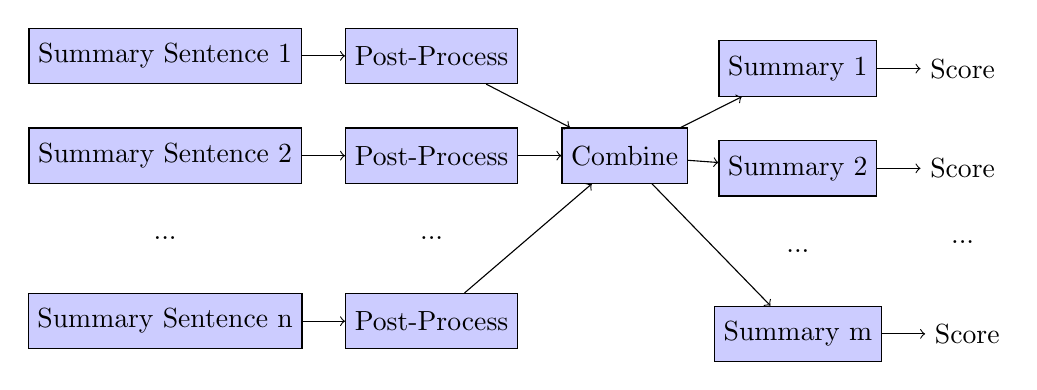
\begin{tikzpicture}[node distance=0.55cm, auto]
\node (summary_sentence_1) [block] {Summary Sentence 1};
\node (summary_sentence_2) [block, below =of summary_sentence_1] {Summary Sentence 2};
\node (summary_sentence_3) [below =of summary_sentence_2] {...};
\node (summary_sentence_4) [block, below =of summary_sentence_3] {Summary Sentence n};
\node (post_process_1) [block, right =of summary_sentence_1] {Post-Process};
\node (post_process_2) [block, below =of post_process_1] {Post-Process};
\node (post_process_3) [below =of post_process_2] {...};
\node (post_process_4) [block, below =of post_process_3] {Post-Process};
\node (combine) [block, right =of post_process_2] {Combine};
\node (summary_1) [block, above right =of combine] {Summary 1};
\node (summary_2) [block, below =of summary_1] {Summary 2};
\node (summary_3) [below =of summary_2] {...};
\node (summary_4) [block, below =of summary_3] {Summary m};
\node (score_1) [right =of summary_1] {Score};
\node (score_2) [below =of score_1, right =of summary_2] {Score};
\node (score_3) [below =of score_2] {...};
\node (score_4) [below =of score_3, right =of summary_4] {Score};
\draw [->] (summary_sentence_1) -- (post_process_1);
\draw [->] (summary_sentence_2) -- (post_process_2);
\draw [->] (summary_sentence_4) -- (post_process_4);
\draw [->] (post_process_1) -- (combine);
\draw [->] (post_process_2) -- (combine);
\draw [->] (post_process_4) -- (combine);
\draw [->] (combine) -- (summary_1);
\draw [->] (combine) -- (summary_2);
\draw [->] (combine) -- (summary_4);
\draw [->] (summary_1) -- (score_1);
\draw [->] (summary_2) -- (score_2);
\draw [->] (summary_4) -- (score_4);
\end{tikzpicture}
\caption{Post-Processing / Scoring Steps}
\label{fig:postprocess_pipeline}
\end{figure}

\section{Summary Creation}
\label{sec:summary_creation}

The output of \textsc{SumASG} is a list of sentences, each of which could potentially appear in the final summary.

\subsection{Post-Processing}

\subsubsection{Grammar}

Because \textsc{SumASG} uses the same capitalization for a given word regardless of its position in the sentence, it means that the first word of each sentence will not be capitalized unless it is a proper noun. We therefore need to fix this, as well as remove the space before each full stop.

Compound nouns, whose hyphen was replaced with an underscore for the internal representation of \textsc{SumASG}, also need to be restored to their grammatically-correct form.

In addition, the task of summarization might have created a sentence where an incorrect verb form is used, or possibly the wrong determiner. To amend this we use a tool called \textbf{\href{https://pypi.org/project/language-check/}{language-check}}, which is able to correct phrases like ``they has an dog" to ``they have a dog".

\subsubsection{Complex Nouns}

One of the optimizations done by the \textsc{Preprocessor} was to combine complex nouns such as ``Peter Little" into their camel-case form ``PeterLittle", so that they would be recognized as a single \textit{token} by \textsc{SumASG}. We now need to expand them back to their original form, as this is how it should be written in English.

\subsection{Combining}

Depending on the length of the original story, we can envision and different number of sentences to be in the summary, as shown below in Table \ref{tab:summary_length}.

\begin{table}[H]
\centering
\begin{tabular}{@{}llll@{}}
\toprule
Story length   & 1-2 & 3-4 & 5+ \\ \midrule
Summary length & 1   & 2   & 3  \\ \bottomrule
\end{tabular}
\caption{Length of a summary depending on the number of sentences in the story}
\label{tab:summary_length}
\end{table}

Once we have grammatically-correct summary sentences and know how many should be kept for the summary (say $n$), we generate all possible order-preserving combinations of length $n$. For instance, such combinations of length 3 for the list $[0,1,2,3]$ would be the following: $[0,1,2]$, $[0,2,3]$ and $[1,2,3]$.

\section{Scoring}
\label{sec:scoring}

As you can imagine, we often end up with a large number of combinations at this phase. We therefore need to determine which of them are best and keep only these.

\subsection{TTR}

To this end, we utilize an NLP metric called TTR (type-token ratio), a measure of lexical density. To provide the most informative summaries possible, we want to maximize the density of unique words.

To calculate a summary's TTR, we divide the number of unique words in the summary by the total number of words. We then divide this by number of unique words in the story and multiply it by a constant, in order to get a more consistent range for our scores.

\subsubsection{Ignored Words}

However, we do not want to neglect summaries using the same determiner, proper noun, or the verb ``to be" multiple times, as these are extremely common in English.

In addition, a story might revolve around a given \textit{topic}, which could be a person. Regarding the former, it could also be the case that the \textsc{Preprocessor} had replaced different synonyms of this \textit{topic} with a unique word.

To get around this, what we can do is to exclude such words from the summary length and number of unique summary words. This way, we no longer require that these ``common" words be unique in a summary. In the following, we will call the enhanced mechanism \textsc{TTR*}.

In Figure \ref{fig:score_example} is an example which illustrates this metric. The summary with the highest final score is considered to be the best. As you can see, there is a greater difference between the summaries when using \textsc{TTR*}, which takes into account the commonly-used building blocks of the English language.

\begin{figure}[H]
\begin{subfigure}{\textwidth}
\begin{displayquote}
Jonathan was a little boy. He was hungry. Jonathan was eating an apple.
\end{displayquote}
\caption{Story}
\vspace{\baselineskip}
\end{subfigure}
\begin{subfigure}{\textwidth}
\begin{displayquote}
\textbf{A.} \underline{Jonathan} \underline{was} \underline{a} hungry boy. \underline{Jonathan} \underline{was} eating \underline{an} apple.\\
\textbf{B.} \underline{Jonathan} \underline{was} \underline{a} little boy. \underline{Jonathan} \underline{was} \underline{a} hungry boy.
\end{displayquote}
\caption{Possible summaries (underlined words will be ignored by \textsc{TTR*})}
\vspace{\baselineskip}
\end{subfigure}
\begin{subfigure}{\textwidth}
\centering
\begin{tabular}{@{}llllllll@{}}
\toprule
Summary & Words & Unique words & TTR & Words* & Unique words* & \textsc{TTR*} & Score \\ \midrule
\textbf{A} & 10    & 8            & 0.8 & 4      & 4             & 1    & 38    \\
\textbf{B} & 10    & 6            & 0.6 & 4      & 3             & 0.75 & 28    \\ \bottomrule
\end{tabular}
\caption{Steps for computing the score}
\end{subfigure}
\caption{Score computation (column headers ending with * pertain to \textsc{TTR*})}
\label{fig:score_example}
\end{figure}

\section{Summary Selection}

\subsection{Proper Nouns}

If a story revolves around a given person and the summary mentions their name, it is preferable for this to be in the first sentence. To put this more clearly, we would like the summary of a biography to introduce the protagonist from the very first sentence. To achieve this, we can simply increase the score of every summary starting with a proper noun by a constant.

\subsection{Top Summaries}

With a more complex story (5 or more sentences), it is highly likely that we will end up with a very long list of possible summaries. As there could be a number of very interesting summaries, we do not want to have to choose exactly one.

Instead, we compute 75th percentile over the scores of all generated summaries, and then discard all those whose score falls below this number. We shall call the remaining summaries \textit{top summaries}.

\subsection{Reference Summaries}

Finally, we want to be sure that our framework generates good summaries, and that the scoring works as intended. Therefore, if a story has a \textit{reference summary}, then we should make sure that there exists a similar \textit{top summary}.

In our implementation, we have chosen to use the BLEU score, which measures how closely the output given by a machine matches a text written by a human. If there exists a \textit{top summary} whose BLEU score with one of the \textit{references} is above a certain threshold, then we consider the summarization to be successful.

\section{Example}
\label{sec:postprocess_example}

An example is shown in Figure \ref{fig:postprocess_score_example} for the story of Peter Little.

The first step is to fix the grammar in the \textit{summary sentences} generated by \textsc{SumASG}, which in this case simply involves capitalizing them and removing the space before the full stop. We also need to restore the proper noun ``PeterLittle" to ``Peter Little". After \textit{combining}, we end up with 35 possible summaries.

The next step is \textit{scoring}, where we augment the standard of ignored words with the case-insensitive \textit{topics} set \texttt{\{"peter", "little"\}} in \textsc{TTR*}. This gives us scores in the range $[10,17]$, 20 of which fall below the 75th percentile of 15.0 and never become \textit{top summaries}.

Finally, we compare these \textit{top summaries} to our \textit{reference summaries} for Peter Little, as mentioned in Chapter \ref{chapter:introduction}. As you can see from the computed BLEU scores, at least one of them achieves a score of at least 0.65, confirming they are close enough to \textit{reference summary} \textbf{B}.

\begin{figure}[H]
\begin{subfigure}{\textwidth}
\begin{displayquote}
Peter Little is famous now.\\
The curious little boy was named Peter Little.\\
There was a curious little boy.\\
Peter Little did school always.\\
Peter Little was curious and serious.\\
Peter Little was curious in astronomy.\\
Peter Little was serious in school.
\end{displayquote}
\caption{Post-processed \textit{summary sentences}}
\end{subfigure}
\begin{subfigure}{\textwidth}
\vspace{\baselineskip}
\begin{displayquote}
\textbf{1.} Peter Little is famous now. Peter Little did school always. Peter Little was curious in astronomy.\\
\textbf{2.} Peter Little is famous now. There was a curious little boy. Peter Little did school always.\\
\textbf{3.} Peter Little is famous now. The curious little boy was named Peter Little. Peter Little did school always.\\
\textbf{4.} Peter Little is famous now. Peter Little did school always. Peter Little was curious and serious.\\
...
\end{displayquote}
\caption{\textit{Top summaries}}
\label{fig:top_score_summaries_example}
\end{subfigure}
\begin{subfigure}{\textwidth}
\vspace{\baselineskip}
\centering
\begin{tabular}{@{}lllllll@{}}
\toprule
Summary     & 1    & 2    & 3    & 4    \\ \midrule
Reference A & 0.4  & 0.38 & 0.32 & 0.38  \\
Reference B & 0.66 & 0.58 & 0.49 & 0.63 \\ \bottomrule
\end{tabular}\caption{BLEU scores for \textit{reference summaries} (summary indices as shown in Figure \ref{fig:top_score_summaries_example})}
\end{subfigure}
\caption{Example of \textit{post-processing} then \textit{scoring} for the story of Peter Little}
\label{fig:postprocess_score_example}
\end{figure}

\section{Expandability}

As you can see from the example in Section \ref{sec:postprocess_example}, there is much room for improvement regarding post-processing.

\subsection{Grammatical Shortcomings}

First of all, we do not revert all the simplification changes made by the \textsc{Preprocessor}. This can lead to a linguistically poor summary, where the same word or name is repeated multiple times, rather than using synonyms or personal pronouns.

Worse than this, we can end up with sentences that would never be written by a human. Because the \textsc{Preprocessor} moves all adverbs to the end of the sentence in which they appear, and is quite eager to homogenize synonyms, summaries generated by \textsc{SumASG*} may end up ``sounding wrong".

\subsection{Better Summary Selection}

Another issue is that we can easily end up with a very large list of summaries. Because the mechanism used to score them is not very advanced, it cannot say for sure that one particular summary is better than all the others. Instead, we usually end up with multiple entries that all have the same maximum score.

We would therefore need to build much more intelligence into this system if we wanted the program to always return a single summary, one that is humans would also consider optimal.

\chapter{Evaluation}
\label{chapter:evaluation}

\section{General Idea}

As the vast majority of modern text summarization frameworks are based on machine learning, it makes sense to compare the performance \textsc{SumASG*} with that of a neural network.

More specifically, we should generate a set of stories which we can give to our framework in order to obtain corresponding summaries. We can then use this as training data for an encoder-decoder, to see if it is able to learn how \textsc{SumASG*} creates summaries.

If the neural network is able to learn to generate similar summaries, then we can consider our framework to be sane.

\section{Story Generation}

\subsection{Libraries}

For this task, we have chosen to use a library called \textbf{\href{http://web.archive.org/web/20190516161631/https://www.clips.uantwerpen.be/pages/pattern-en}{Pattern}}, which allows us to conjugate verbs, as well as toggle nouns between singular and plural.

We also take advantage of the \textbf{\href{https://www.datamuse.com/api/}{Datamuse API}}, which lets us find words which are semantically related to a given word in a certain way.

\subsection{Datasets}

In order to generate the required number of stories, we have used words from \href{http://www.wordfrequency.info/}{wordfrequency.info}. This database contains 5,000 individual English words, of which 1,001 are verbs, 2,542 nouns and 839 adjectives.

For each story we chose a noun from our dataset, which we shall refer to as the \textit{topic}. We then construct four sentences which revolve around this \textit{topic}.

\subsection{Sentence Generation}

We will begin by detailing how each sentence is generated, starting with a few necessary definitions. Throughout this section, it is important to keep in mind that the goal here is to create a story that is as lexically and semantically coherent as possible, which is tricky to do algorithmically.

\subsubsection{Definitions}

\begin{definition}[Hyponym]
A \textit{hyponym} is a word with more specific meaning than another word; ``computer" is a \textit{hyponym} of ``machine".
\end{definition}

\begin{definition}[Hypernym]
A \textit{hypernym} is a semantic superclass of a word; ``vehicle" is a \textit{hypernym} of ``bus".
\end{definition}

\begin{definition}[Holonym]
A \textit{holonym} of something is one of its constituents; ``lightbulb" is a \textit{holonym} of ``lamp".
\end{definition}

\begin{definition}[Meronym]
A \textit{meronym} is an object which something is part of; ``house" is a \textit{meronym} of ``kitchen".
\end{definition}

\subsubsection{Lexical Common Nouns}

Along with the story's \textit{topic}, we also generate a set of \textit{lexical common nouns}. If the \textbf{Datamuse API} is able to find \textit{synonyms} of our \textit{topic} which also belong to our dataset of nouns, then these become the story's \textit{lexical common nouns}.

In addition, we query from the \textbf{Datamuse API} for verbs that are related to the chosen \textit{topic}. This becomes our set of \textit{lexical verbs}. If it is empty, then we make it the singleton set containing the verb ``to be".

Since we don't know how general or specific this randomly selected \textit{topic} is, we may not find any. In this case, we try the same procedure for \textit{hypernyms} and finally \textit{hyponyms}. If we still are unable to find any (which is very rare), then we pick a new random \textit{topic}.

\subsubsection{Subject}

For the \textit{subject} of a sentence, we draw a noun from our \textit{lexical common nouns}.

If this word is singular, then we need a determiner, which can be either ``the" or ``a".

We also ask the \textbf{Datamuse API} to find us an adjective which is often modified by the chosen \textit{subject} noun, and is part of our dataset of words. If none is found, then we do not need to use an adjective.

\subsubsection{Verb}

We chose a verb at random from our set of \textit{lexical verbs}, conjugating it in the past tense so that it agrees with the sentence's \textit{subject}.

\subsubsection{Object}

For the \textit{object} of our sentence, we look at the \textit{subject} and \textit{verb}. Using the \textbf{Datamuse API} we try and find a noun which often appears after the chosen \textit{verb}, and which is related to our \textit{topic} as well as all nouns we have used thus far in the story. With 50\% probability we ask it to be a \textit{holonym} of the \textit{subject} noun, otherwise it should be a \textit{meronym}.

In the same way as we did for the \textit{subject}, we try and find an adjective often modified by the chosen noun. Sometimes it will be the case that no noun was found, but it is possible in English to have an adjective as the only word in the \textit{object}.

The determiner is added as for the \textit{subject}; if there is no noun we do not use one.

\subsubsection{Example}

We take the example of generating a sentence for a story whose \textit{topic} is ``soccer". In this case, the \textit{lexical common nouns} are a singleton set containing the word ``football". Here also have two \textit{lexical verbs}: ``to match" and ``to pitch".

For the \textit{subject}, we can choose the \textit{lexical common noun} ``football"; an adjective commonly used to modify it is ``professional". Since the noun here is singular, we can use the determiner ``a".

We can then pick ``to pitch" as the \textit{verb}, which becomes ``pitched" when conjugated in the past tense.

For the \textit{object}, we take into account our \textit{topic} ``soccer", to find a \textit{holonym} of ``football" which often appears after the \textit{verb} ``pitched". In this case the \textbf{Datamuse API} returns the word ``reception", resulting in the adjective ``warm" being chosen to accompany it.

After repeating this process three more times, we end up with the below story. As you can see, \textsc{SumASG\textsubscript{2}} would be able to combine the two last sentences, but the result of this may or may not make it into the summary we choose.

\begin{displayquote}
The professional football matched a place. A professional football pitched the warm reception. A professional football matched a warm reception. A professional football matched a wonder.
\end{displayquote}

\subsection{Action Creation}

Using a Python script, we generate the corresponding \textit{actions} as would \textsc{SumASG\textsubscript{1}}, creating the necessary additional leaf nodes for our general grammar in ASG. We do not use \textsc{SumASG\textsubscript{1}} to do this mainly for performance reasons, but also as it is not necessary. Because of the way in which we have created our stories, \textit{simplification} would not change the sentence structure whatsoever, and no sentences would be considered irrelevant (or off-topic) by the \textsc{Preprocessor}.

\subsection{Summary Generation}

For each story, we feed the generated \textit{actions} and leaf nodes directly into \textsc{SumASG\textsubscript{2}}, skipping the first half of the \textsc{SumASG*} pipeline. After \textit{scoring}, we pick an entry at random from the \textit{top summaries}.

\section{Neural Network}

\subsection{Datasets}

Using the mechanism described above, we generate a number of story/summary pairs: 1796 to be used for training, 199 for validation and 5 for testing.

\subsection{Tools}

To allow for greater flexibility, we have chosen to use a highly versatile open-source framework called \textbf{\href{https://github.com/OpenNMT/OpenNMT-py}{OpenNMT-py}} for training our neural network.

In addition, we preprocess the data using Stanford's \textbf{\href{https://nlp.stanford.edu/projects/glove/}{GloVe}} pre-trained word embeddings, giving our network a head-start when it comes to semantics.

\subsection{Encoder-Decoder Architecture}

Our \textit{encoder} and \textit{decoder} share embeddings for a vocabulary of size 7295, which is internally represented using a vector of size 250. They both use a two-layer LSTM with \textit{dropout} of 0.25. Additionally, our \textit{decoder} uses \textit{global attention}.

\subsection{Training}

The neural network was trained using an Adam optimizer with a \textit{learning rate} of 0.0005 and \textit{batch size} of 50. This was done over a period of 10,000 steps (i.e., 200 epochs), validating every 10 epochs. It took 39 epochs for training accuracy to reach 99\%, while validation accuracy slowly increased over time to reach about 53\% at the end.

\subsection{Results}

At first glance, it may seem as though this \textit{encoder-decoder} was overfitting the training data. However, it is important to keep in mind that multiple valid summaries may exist for a given input story, and that the target summary was not necessarily the same as the one generated by the network.

Unfortunately, due to framework constraints, it is impossible to provide the training script with multiple target summaries. However, it is simple to run the trained network on our test stories, and then compare the results to the many summaries generated by \textsc{SumASG*}.

\begin{figure}[H]
\begin{subfigure}{\textwidth}
\begin{displayquote}
\textbf{1.}\\
\textbf{2.}\\
\textbf{3.}\\
\textbf{4.}\\
\end{displayquote}
\caption{\textit{Test stories}}
\end{subfigure}
\begin{subfigure}{\textwidth}
\vspace{\baselineskip}
\begin{displayquote}
\textbf{1.}\\
\textbf{2.}\\
\textbf{3.}\\
\textbf{4.}\\
\end{displayquote}
\caption{\textit{Summaries generated by the \textit{encoder-decoder}}}
\end{subfigure}
\begin{subfigure}{\textwidth}
\vspace{\baselineskip}

\caption{Maximum BLEU scores between \textit{encoder-decoder} summary and \textsc{SumASG*} summaries}
\end{subfigure}
\caption{TODO}
\label{fig:neural_network_testing}
\end{figure}

\textcolor{red}{\textbf{\hl{TODO}}}

\section{Takeaways}

After having done this experiment, we can make the following assessments:

\begin{itemize}
\item Using a state-of-the-art neural network architecture, it is possible to learn some of the summarization rules that have been programmed into \textsc{SumASG*}.
\item A neural network needs vast amounts of data and some time to learn an approximation to what is a summary, whereas in \textsc{SumASG} the definition of summary is built-in.
\item A neural network needs to be trained again for each new summarization rule we would like it to learn, while \textsc{SumASG*} can be used directly after expanding it.
\item The coherence of summaries produced by a neural network is extremely tied to the nature and diversity of the training corpus, whereas \textsc{SumASG*} performs similarly on all stories whose structure it can parse.
\item While \textsc{SumASG*} always uses information from the story to construct its summary, a summary from a neural network can sometimes include irrelevant words or the unknown \textit{token}.
\item A neural network will always produce an output sequence regardless of whether the input is valid English, whereas \textsc{SumASG*} will ignore anything that it was not programmed to understand.
\end{itemize}

\textcolor{red}{\textbf{\hl{TODO make into a table?}}}

For for each story:
1. Pick predefined lexical field (topic)
2. Pick a single pronoun (p)
3. Pick a single proper noun (pn)
4. For each sentence:
    - Subject: p, pn, or synonym/hyponym/hypernym of topic with optional common adjective for it
    - Verb: verb from same lexical field as topic if possible, otherwise random
    - Object: p, pn, or holonym/meronym of subject with lexical field of currently used common nouns
    

- Compare with NN
    1. Randomize action(...) to generate summary(...) on trained ASG
    2. Train NN to generate same summary(...)
    3. Show framework is sane and expandable (computationally tractable)
    4. Compute Rouge score (PyRouge, must clone repo into project) on ASG and NN

\chapter{Literature Review}
\label{chapter:literature_review}

\section{Summarization Levels}

Depending on how much text analysis is done, we identify three different levels of summarization \cite{lloret_text_2008}. Many current systems employ what is called a \textit{hybrid approach}, combining techniques from different levels.

\subsection{Surface Level}

On a \textit{surface level}, little analysis is performed, and we rely on keywords in the text which are later combined to generate a summary. Techniques which are common include:

\begin{itemize}[nolistsep]
\item \textit{Thematic features} are identified by looking at the words that appear the most often. Usually, the important sentences in a passage have a higher probability of containing these \textit{thematic features}.
\item Often, the \textit{location} of a sentence can help identify its importance; the first and last sentences are generally a good indicator for the respective introduction and conclusion of a document. Moreover, we may want to make use of the title and heading (if any) to find out which topics are most relevant.
\item \textit{Cue words} are expressions like ``in this article" and ``to sum up"; these can give us a clue as to where the relevant information is.
\end{itemize}

\subsection{Entity Level}

A more analytic approach can be done at an \textit{entity level}, where we build a model of a document's individual entities and see how they relate. Common techniques include:

\begin{itemize}[nolistsep]
\item \textit{Similarity} between different words (or phrases), whether it be synonyms or terms relating to the same topic.
\item \textit{Logical relations} involve the use of a connector such as ``before" or ``therefore", and tell us how the information given by such connected phrases relates.
\end{itemize}

\subsection{Discourse Level}

Finally at a \textit{discourse level} we go beyond the contents of a text, exploiting its structure instead. Some of the things we can analyze are:

\begin{itemize}[nolistsep]
\item The \textit{format} can be taken into account to help us extract key information. For example, in a rich-text document we may want to pay close attention to terms that are underlined or italicized.
\item The \textit{rhetorical structure} can tell us whether the document is argumentative or narrative in nature. In the latter case a more concise description of the text's contents would suffice, while the former would involve recounting the key points and conclusions made by the author.
\end{itemize}

\section{Semantic Analysis Methods}

\subsection{Combinatory Categorial Grammar} \label{ssec:ccg}

In a paper from 2019 \cite{steedman_combinatory_nodate}, the author introduces Combinatory Categorial Grammar (CCG), an efficient parsing mechanism to get to the underlying semantics of a text in any natural language. It is combinatory in the sense that it uses functional expressions such as $\lambda p.p$ in order to express the semantics of words.

In CCG, every word, written in English in its \textit{phonological form}, is assigned a \textit{category}. Furthermore, a \textit{category} is comprised of the word's \textit{syntactic type} and \textit{logical form}. As shown in Figure \ref{fig:ccg_forms}, the former gives all the conditions necessary for a word to be combined with another, and the latter shows in a simpler form its representation in logic. The \textit{phonological form} comes from the input text, the \textit{syntactic type} is used in the process of conducting semantic analysis, and finally the \textit{logical form} is the result of parsing a passage.

\begin{figure}[H]
\centering
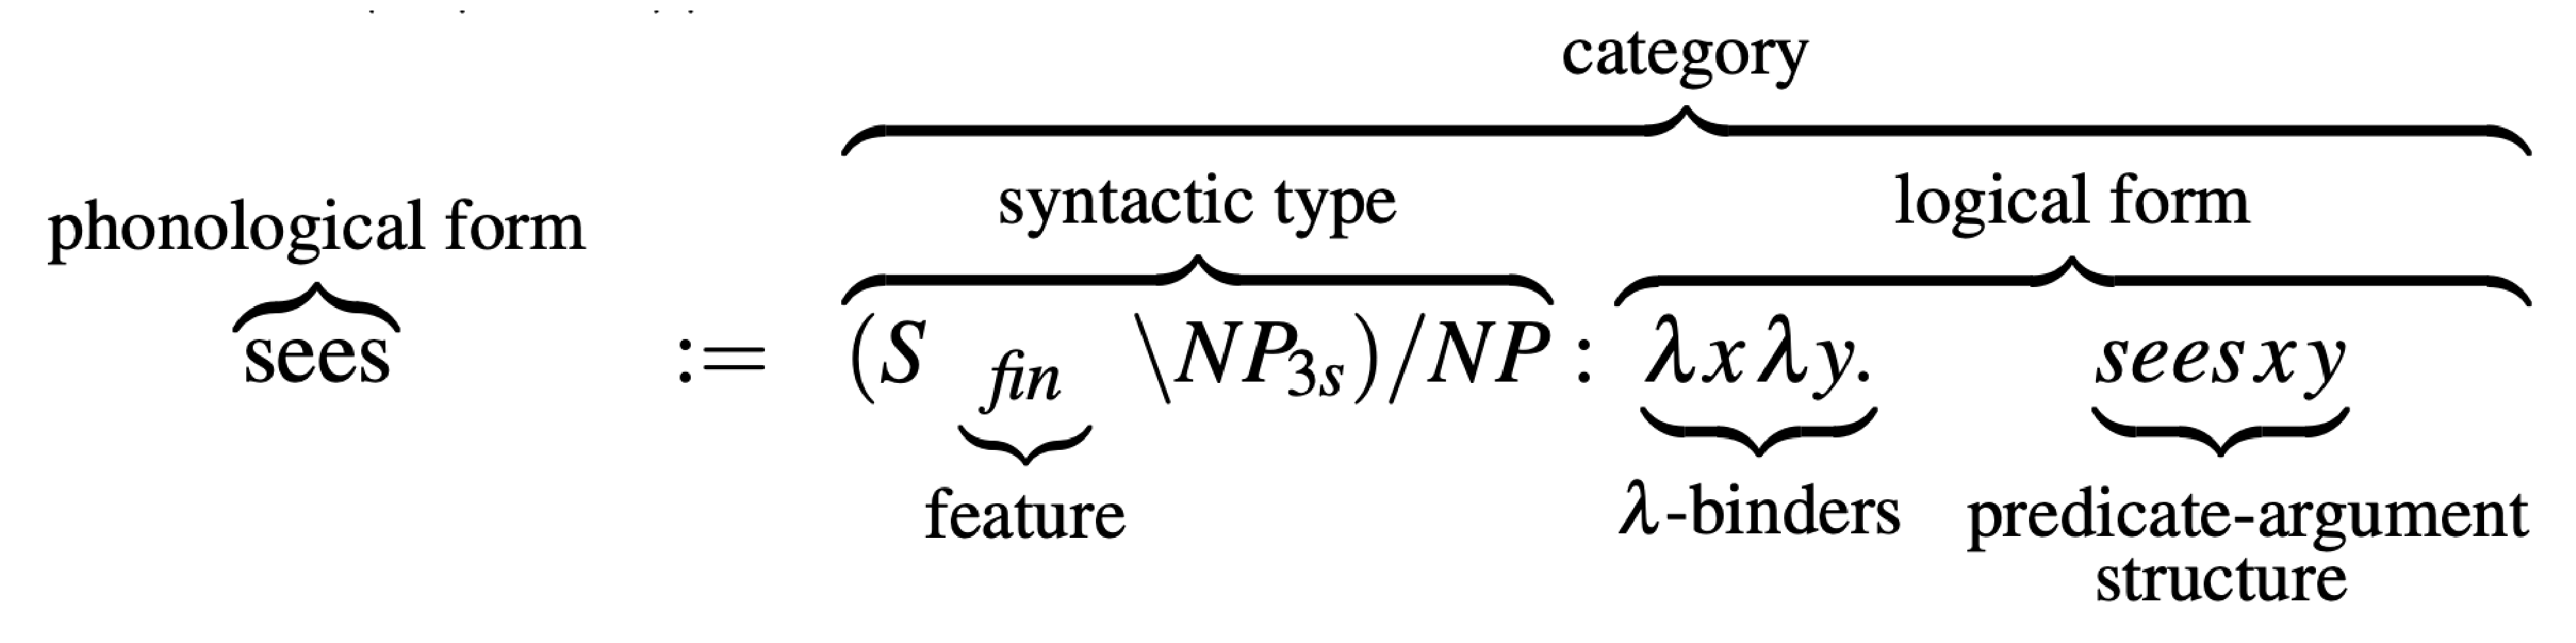
\includegraphics[width=0.8\textwidth]{ccg_forms.eps}
\caption{\cite{steedman_combinatory_nodate} Diagram explaining the mains terms used in CCG}
\label{fig:ccg_forms}
\end{figure}

In the \textit{syntactic type} of a word, the forward slash / indicates forward application to combine terms, while \textbackslash \ indicates backward combination. If there is no slash, then the expression can be thought of as a clause, and it can combine with any rule.

\begin{itemize}[nolistsep]
\item $X/Y:f \quad Y:a \implies X:fa$\quad($>$)
\item $Y:a \quad X\backslash Y:f \implies X:fa$\quad($<$)
\end{itemize}

\mbox{}

There also exists a \textit{morphological slash} \textbackslash\textbackslash, which restricts application to lexical verbs, ruling out auxiliary verbs (whose role is purely grammatically, hence they do not play any part in providing information). The \textit{morphological slash} can be used when dealing with reflexive pronouns such as ``themselves". Furthermore, combining rules directly correlates to obtaining a simpler \textit{logical form} with fewer bound variables, as can be seen in Figure \ref{fig:ccg_derivations}.

\begin{figure}[H]
\centering
\begin{subfigure}{0.3\textwidth}
\centering
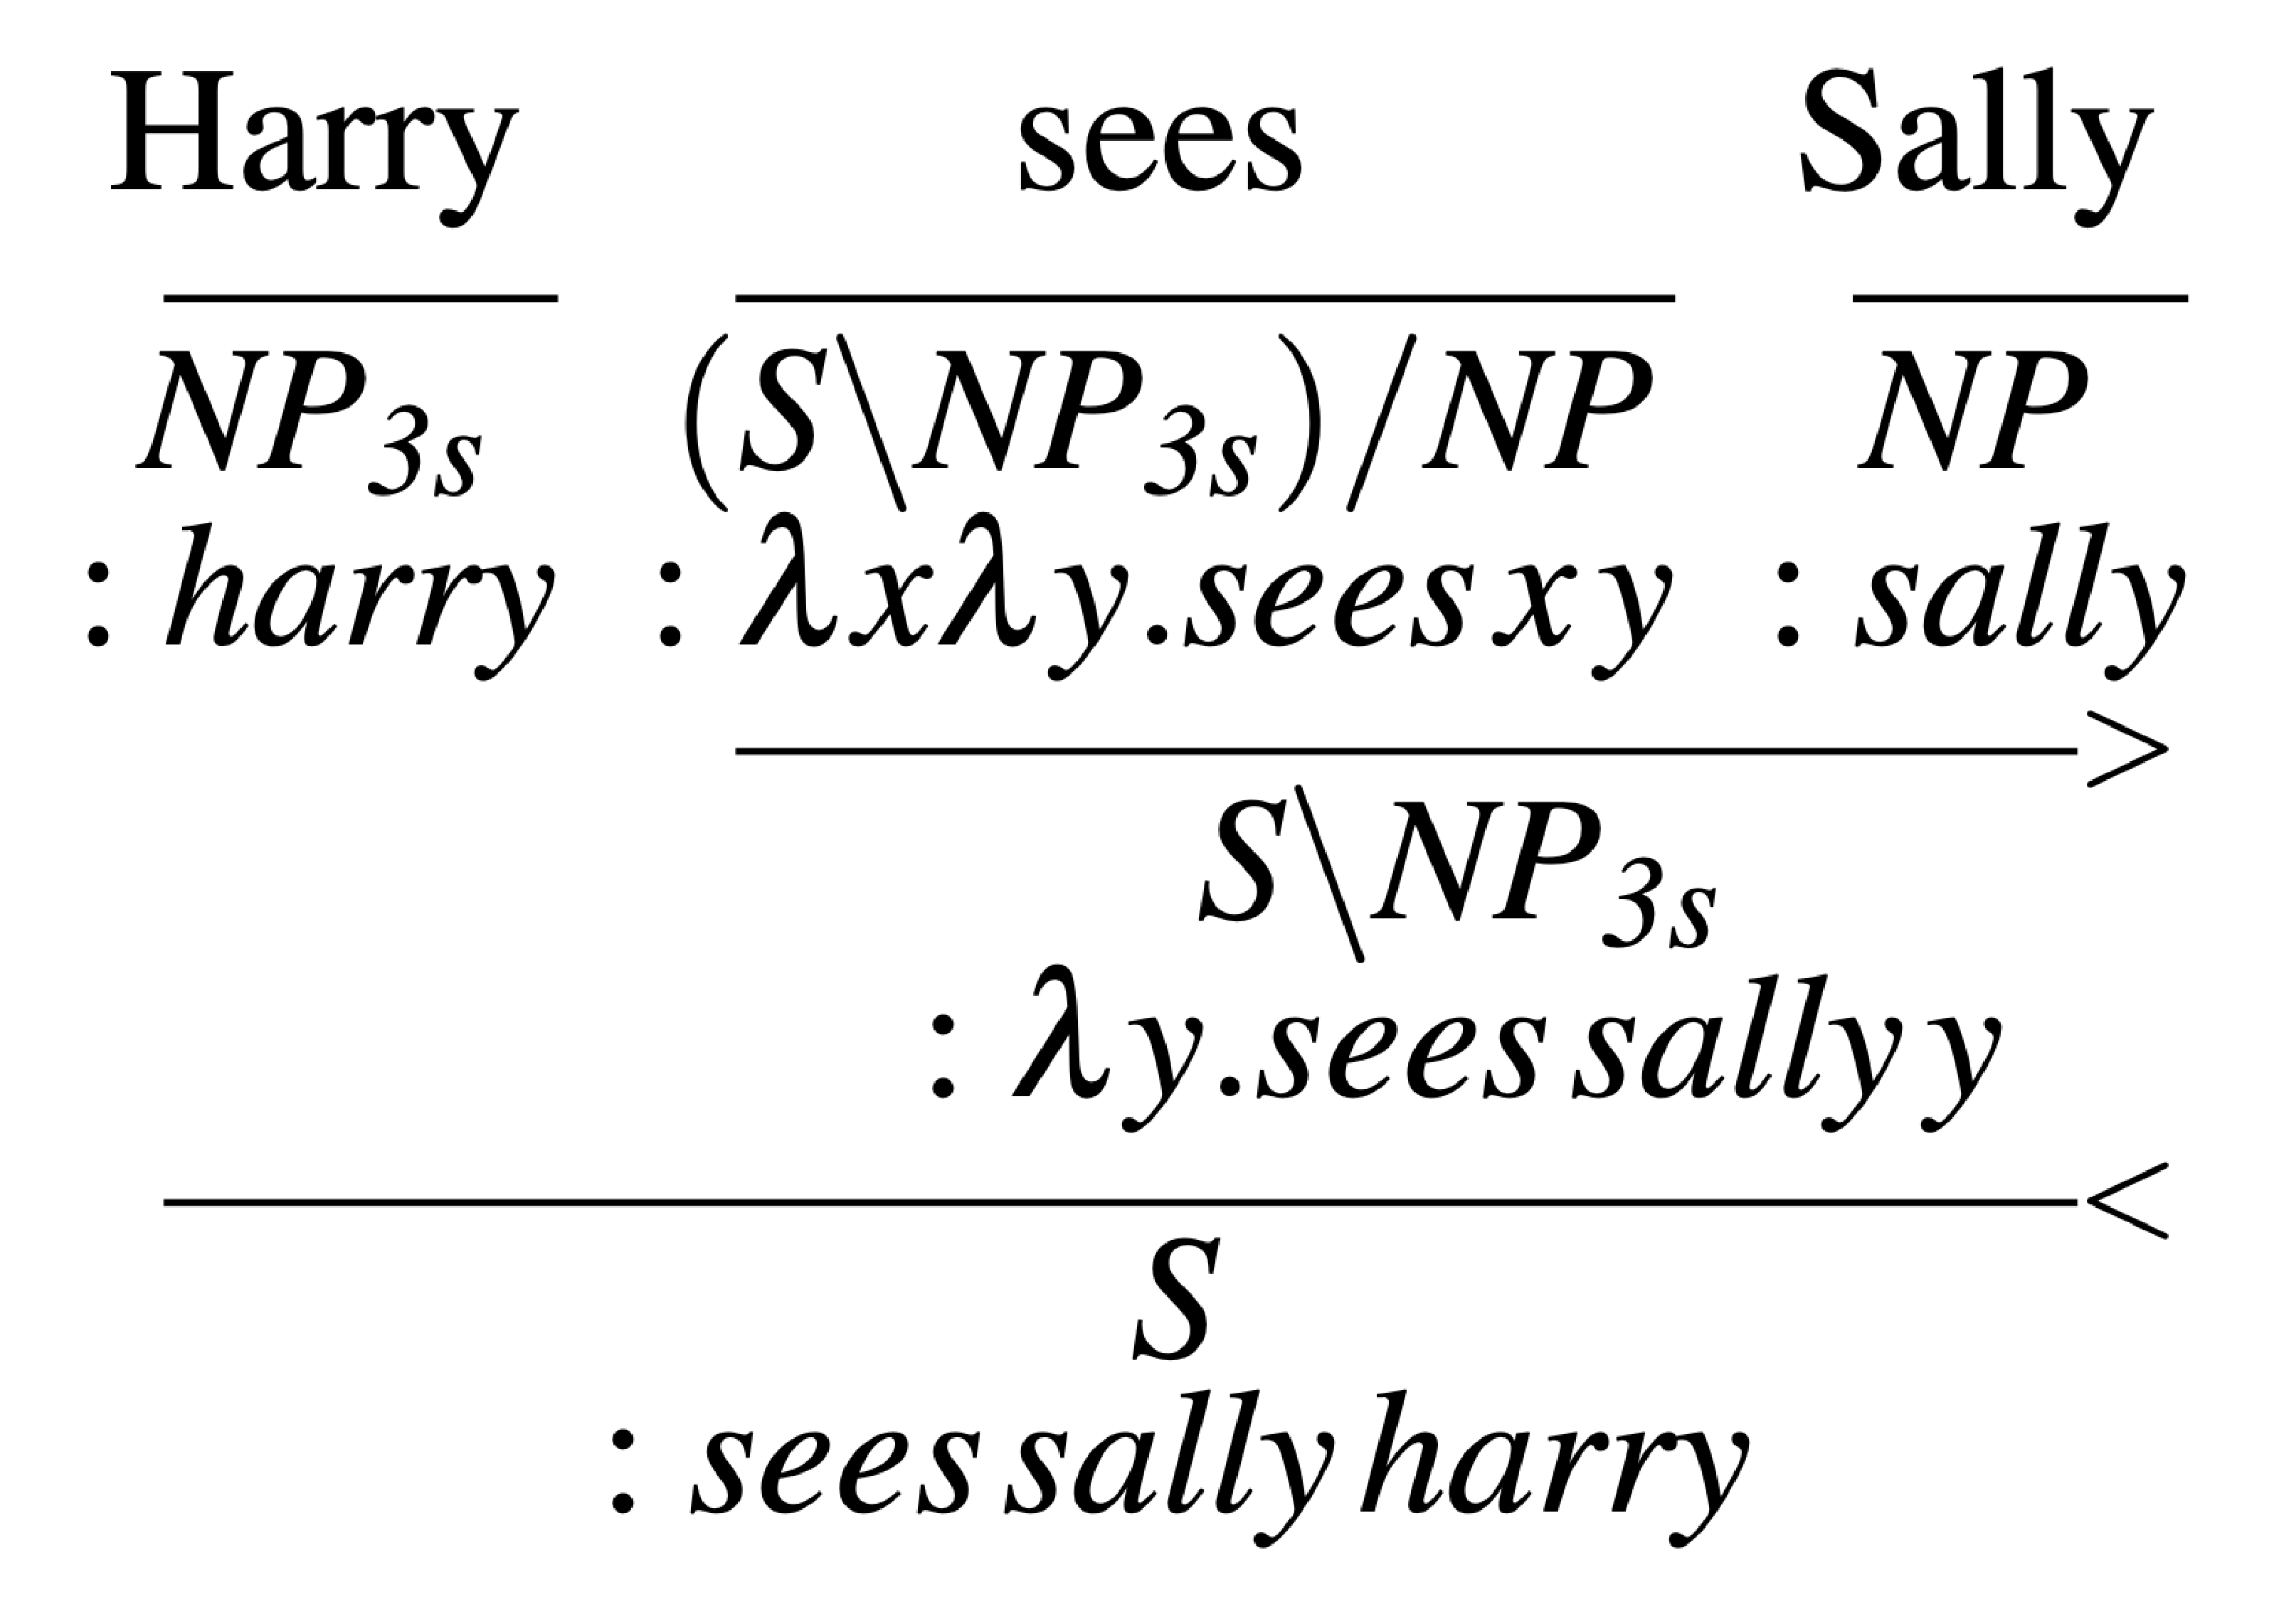
\includegraphics[width=\textwidth]{ccg_basic_derivation.eps}
\caption{\cite{steedman_combinatory_nodate} Basic clause}
\end{subfigure}
\begin{subfigure}{0.6\textwidth}
\centering
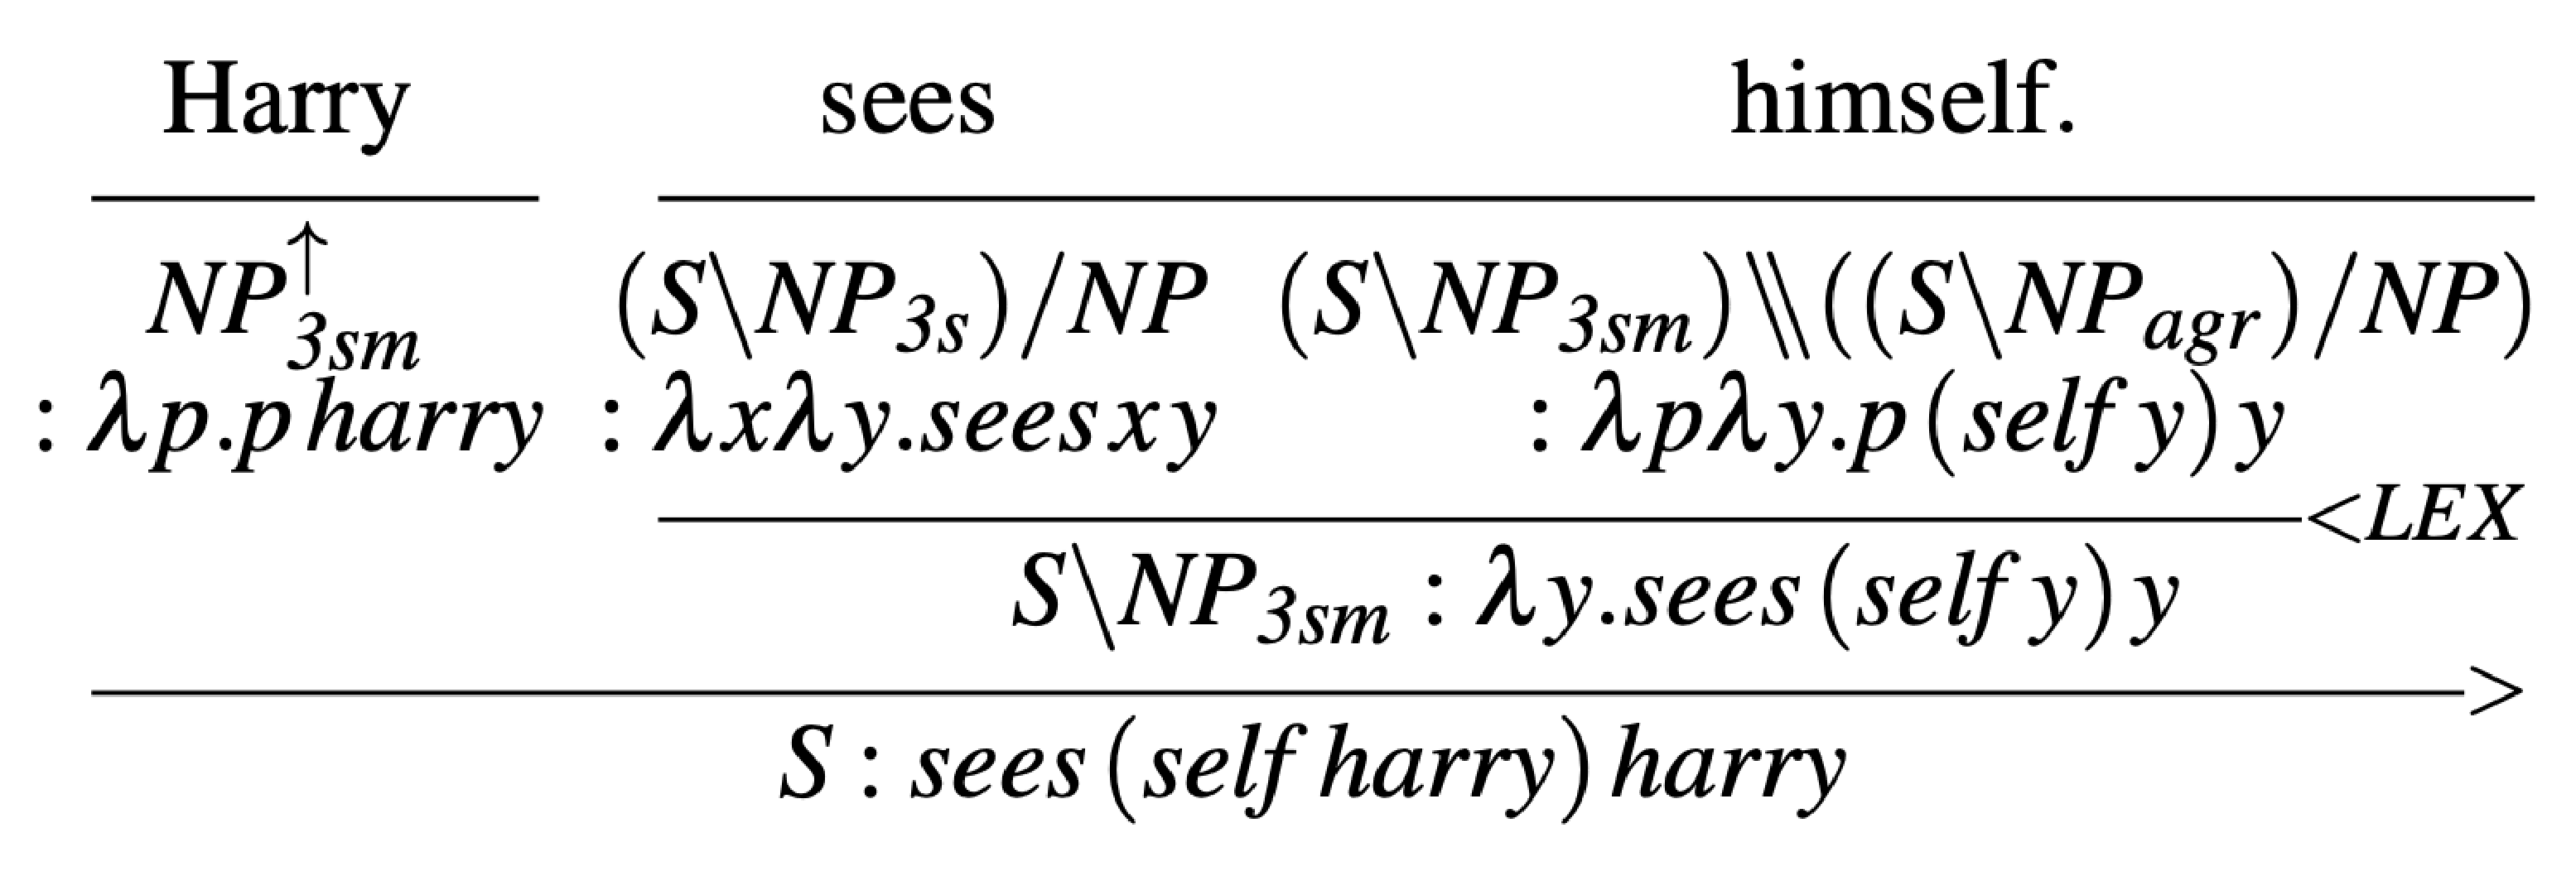
\includegraphics[width=\textwidth]{ccg_reflexive_derivation.eps}
\caption{\cite{steedman_combinatory_nodate} Reflexive transitive clause}
\end{subfigure}
\caption{Examples of derivations in CCG}
\label{fig:ccg_derivations}
\end{figure}

There exist more advanced syntactic rules in CCG, which we shall not go into detail about for the purposes of brevity. However with the basic rules that we explained, you can easily see how this parsing mechanism could be an efficient way to get to the underlying semantics of a sentence. Although the \textit{syntactic type} may seem complicated, it would allows us to get a very precise understanding of English grammar, as well as obtain a simple and consistent \textit{logical form} at the end.

\section{Existing Approaches}

\subsection{MCBA+GA And LSA+TRM}

In a paper by Yeh et al. \cite{yeh_text_2005}, two different methods are put forward for text summarization. The first is the modified corpus-based approach (MCBA), which uses a score function as well as the \textit{genetic algorithm}, while the second (LSA+TRM) utilizes \textit{latent semantic analysis} (LSA) with the aid of a \textit{text relationship map} (TSA).

\mbox{}

In order to understand MCBA, we must first mention corpus-based approaches, which rely on machine learning applied to a corpus of texts and their (known) summaries. In the \textit{training phase} important features (such as sentence length, position of a sentence in a paragraph, uppercase word...) are extracted from the \textit{training corpus} and used to generate rules. In the \textit{test phase} the learned rules are applied on the \textit{training corpus} to generate corresponding summaries. Most approaches rely on computing a weight for each unit of text, this is based on a combination of a unit's features.

The MCBA builds on the basic corpus-based approach (CBA) by ranking sentence positions and using the genetic algorithm (GA) to train the score function. In the first case, the idea is that the important sentences of a paragraph are likely to have the same position in different texts, such as the first sentence (introduction) and the last one (summary). Depending on a sentence's position, a \textit{rank} (from $1$ to some $R$) is assigned, and used to compute a score for this feature. The paper also discusses other features, whose corresponding scores, along with the aforementioned \textit{rank}, are used to compute a weighted sum of all scores. Only the highest scoring sentences are retained in order to form the summary.

Moreover, the \textit{genetic algorithm} (GA) is used to obtain suitable weights, where a \textit{chromosome} is defined by a set of values for all the features weights. Using the notions of \textit{precision} (proportion of predicted positive cases that are correctly real positives) and \textit{recall} (proportion of real positive cases that are correctly predicted positive) \cite{powers_evaluation_2011}, a so-called \textit{F-score} is computed to define the fitness for each chromosome. By combing two \textit{chromosomes} to generate children, where the fittest parents are most likely to mate, we end up (after some number of generations) with a set of feature weights suitable for the corpus in question.

\mbox{}

On the other hand, the LSA+TRM approach comprises four major steps: \textit{preprocessing} (1), \textit{semantic model analysis} (2), \textit{text relationship map construction} (3) and \textit{sentence selection} (4).

In step (1), sentences are decomposed according to their punctuation, as well as divided into keywords.

In step (2), a \textit{word-by-sentence matrix} is computed on the scale of the entire document (or corpus). This  gets factorized and reduced to leave out words which do not occur often, then turned into a \textit{semantic matrix} linking words to their according relevance with each sentence.

In step (3), the \textit{semantic matrix} is converted to a \textit{text relationship map}. A \textit{text relationship map} is a graph comprised of nodes, each one represents a sentence or paragraph. A link exists between any two which have high semantic similarity, and the idea is that nodes with many links are likely to cover the main topics of the text.

Finally, step (4) uses the \textit{text relationship map} to pick out the most important sentences for the summary. Figure \ref{fig:lsa_trm_diagrams} may help you visualize how this works.

\begin{figure}[H]
\begin{subfigure}{0.5\textwidth}
\includegraphics[width=\textwidth]{lsa_trm_diagram.eps}
\caption{\cite{yeh_text_2005} Overall process}
\end{subfigure}
\begin{subfigure}{0.5\textwidth}
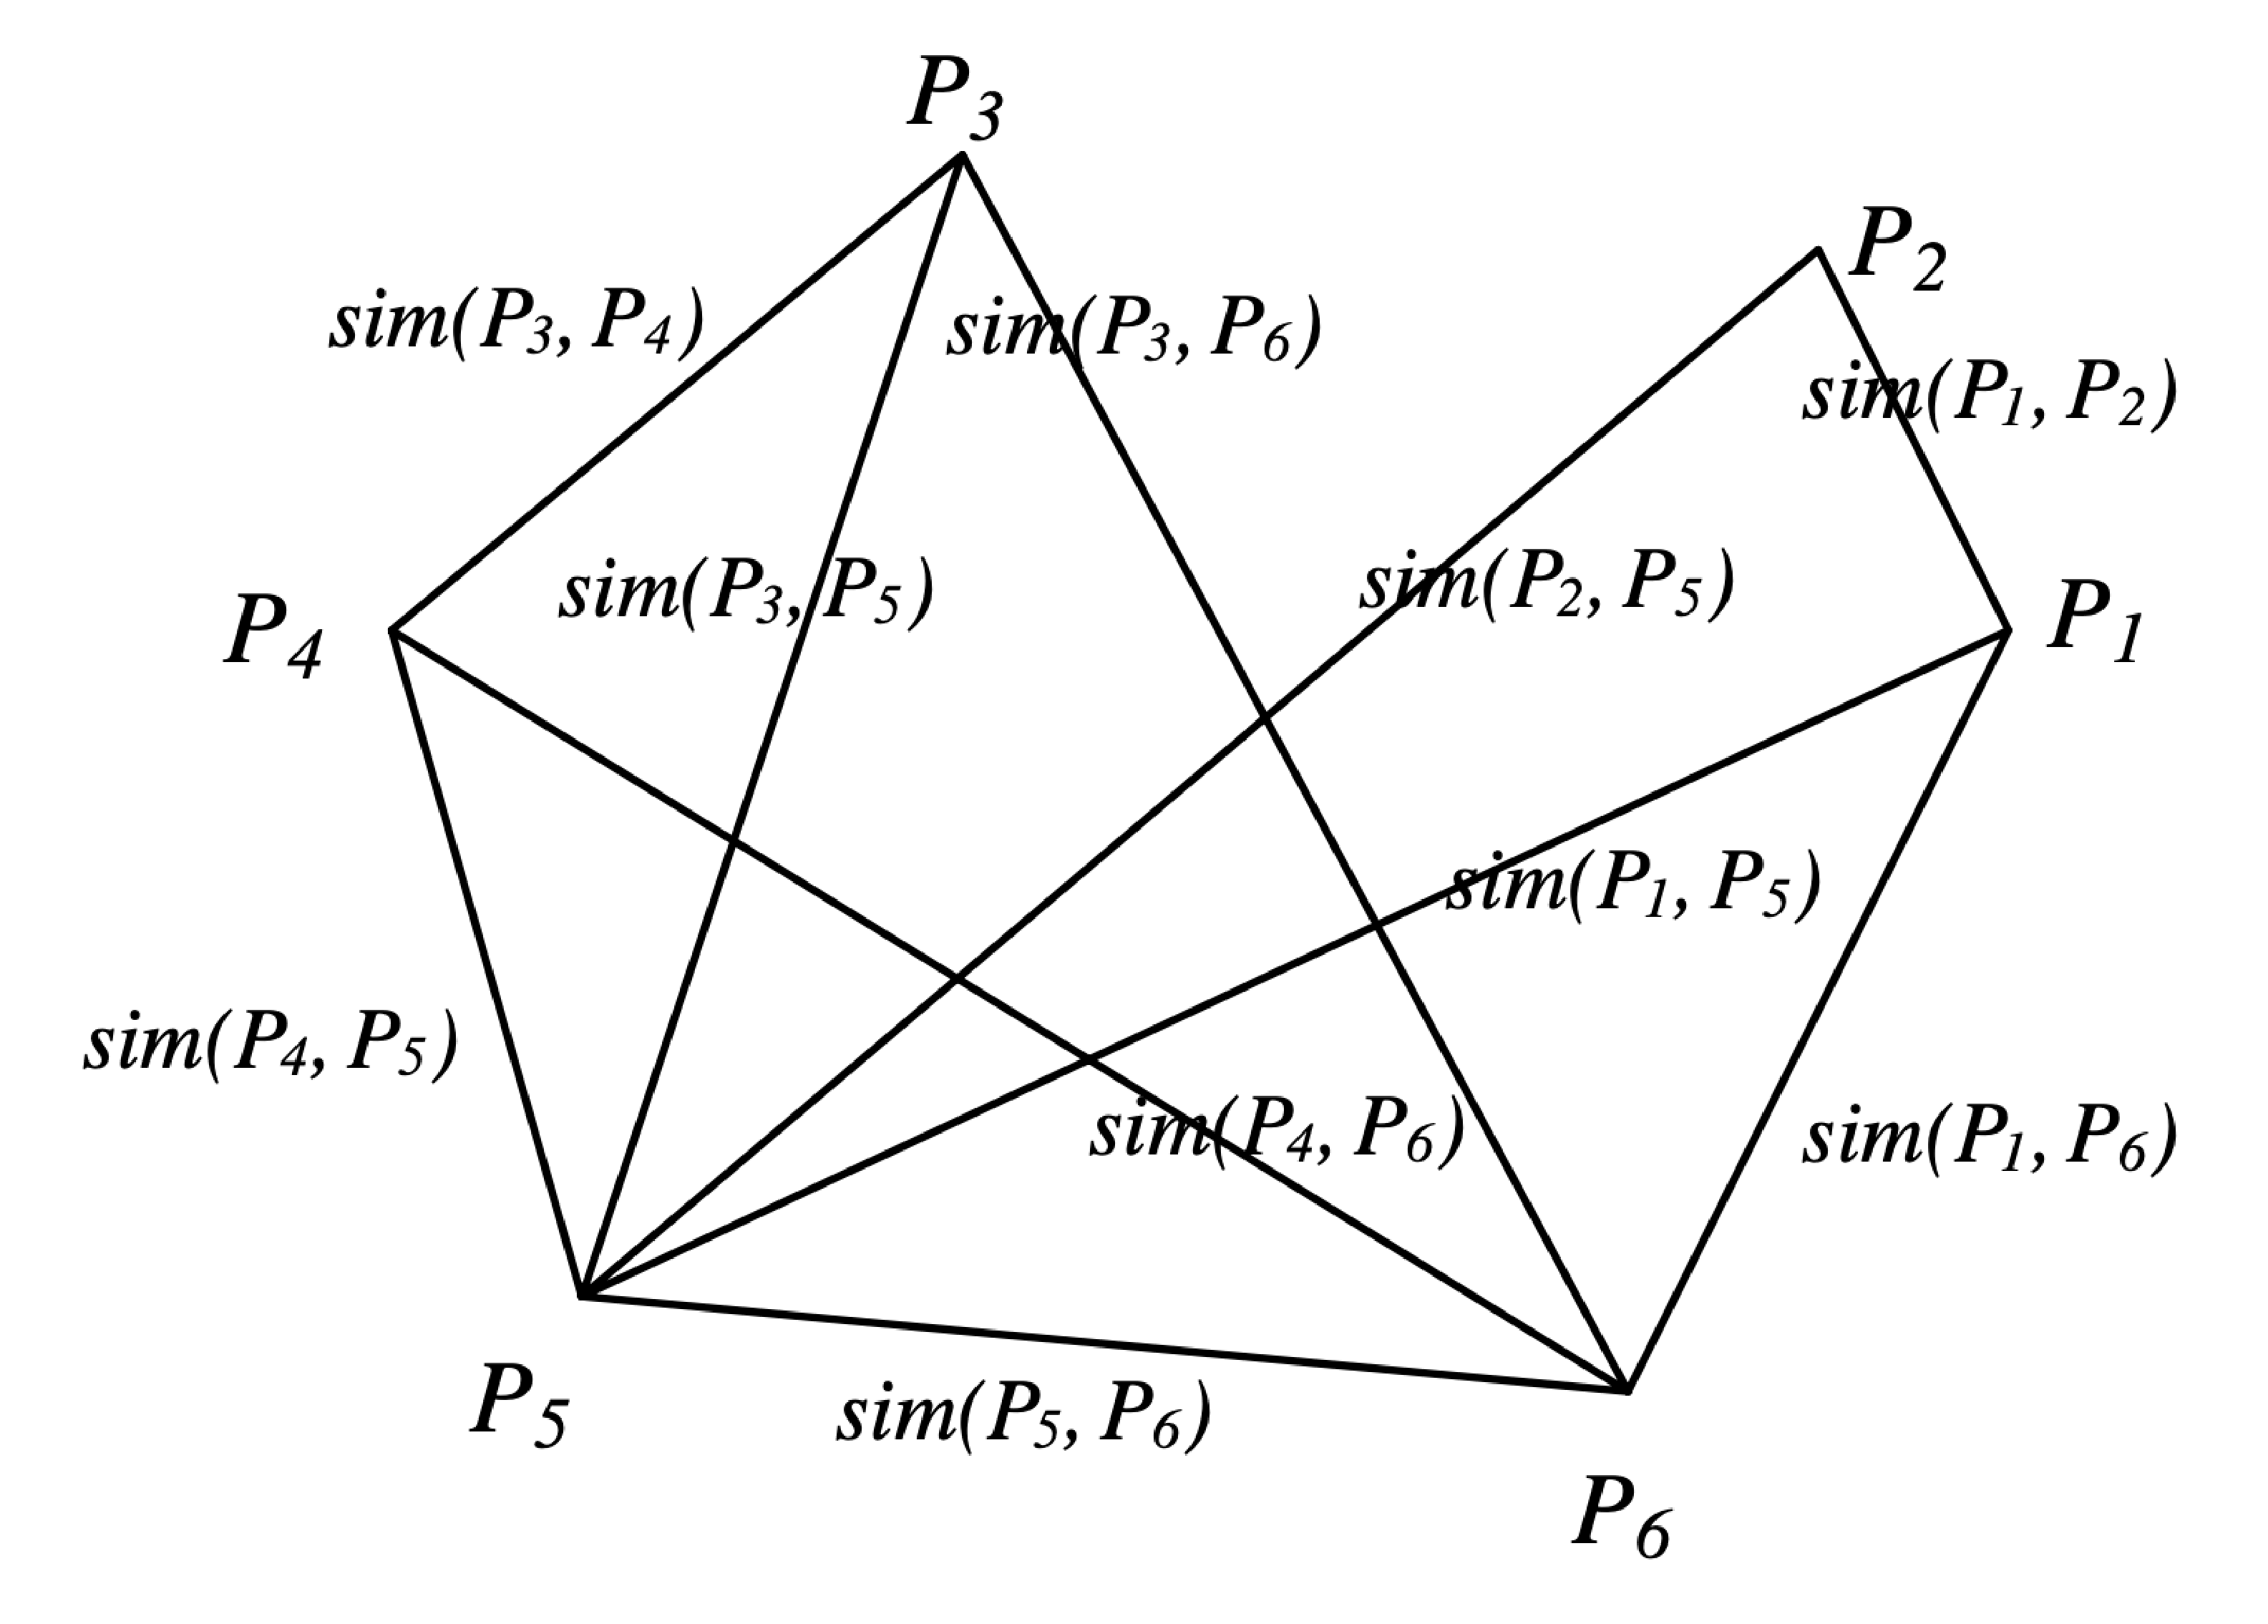
\includegraphics[width=\textwidth]{text_relationship_map_diagram.eps}
\caption{\cite{yeh_text_2005} Example of a text relationship map}
\end{subfigure}
\caption{LSA+TRM approach, diagrammatically}
\label{fig:lsa_trm_diagrams}
\end{figure}

\textit{Compression rate} (CR) is a proportion describing the size of the summary with respect to the size of the original text.

After evaluating both approaches on a news article corpus, it was found that MCBA outperforms the basic CBA by around 3\%, confirming the hypothesis that the position of a sentence plays a role in its importance. Furthermore, MCBA+GA performs around 10\% better than MCBA.% However, the difference in genre between the \textit{training corpus} and \textit{test corpus} has an influence on the performance of GA.

Concerning LSA+TRM, it was found that on a per-document level this approach outperformed simply using TRM with the sentence keywords rather than LSA by almost 30\%. It was thus concluded that LSA helps get a better semantic understanding of a text.% On a corpus-level, this performance improvement is only around 20\%.

Comparing the two approaches highlighted in the paper, it is mentioned that performance is similar, although LSA+TRM is easier to implement than MCBA in single-document level as it requires no preprocessing, and in some optimal cases performs up to 20\% better. Although the former approach is more computationally expensive, it is more adept at understanding the semantics of a text because it does not rely on the genre of the corpus that was used for training. In both cases though, performance improves as CR increases.

\mbox{}

As our solution will rely on ASG, no machine learning will be needed. However, the first approach is still interesting in the sense that it uses a certain number of important features to identify the important sentences of a passage. In our approach, we may want to use some of these metrics to construct the summary.

From the second approach, the main takeaways are the storage mechanisms in use such as the \textit{semantic matrix} and \textit{text relationship map}. In our system we may also want to use the idea that sentences or \textit{chunks} which are semantically similar to many others in the \textit{text relationship map} are likely to cover the main topics of a passage.

Finally, we notice that the approach based on machine learning (MCBA) gives summaries of inferior quality in general, confirming that the use of ASG is a good choice. In addition, it was found that the longer the summary (higher CR), the more accurate it is, so we must be particularly careful when generating one to two sentence summaries.

\subsection{Lexical Chains}

In a paper about \textit{lexical chains} \cite{barzilay_using_1997}, the authors describe a method which relies on semantic links between words. The idea is that we establish chains of related words, in order to learn what a text is about.

In order to create such a chain, the algorithm begins by choosing a set of \textit{candidate words} for the chain. These \textit{candidate words} are either nouns, or \textit{noun compounds} (such as ``analog clock"). Starting from the first word, the task is to find the next related word which has a similar meaning (a dictionary is used here). If the word has multiple senses, then the chain gets split into multiple interpretations; this process continues until we have analysed all \textit{candidate words}.  For instance, the word ``person" can be interpreted as meaning a human being (\underline{interpretation 1}), or as a grammatical term used for pronouns (\underline{interpretation 2}). An example for the below text is shown in Figure \ref{fig:lexical_chain_example}.

\begin{displayquote}
\textbf{Mr.} Kenny is the \textbf{person} that invented an anesthetic \textbf{machine} which uses \textbf{micro-computers} to control the rate at which an anesthetic is pumped into the blood. Such \textbf{machines} are nothing new. But his \textbf{device} uses two \textbf{micro-computers} to achieve much closer monitoring of the \textbf{pump} feeding the anesthetic into the patient. \cite{barzilay_using_1997}
\end{displayquote}

Furthermore, \textit{lexical chains} are attributed a \textit{strength}, which is based on three criteria: repetition (of the same word), density (the concentration of chain members in a given portion of the text) and length (of the chain). For instance, the \textit{lexical chain} beginning with the word ``machine" shown in Figure \ref{fig:lexical_chain_example} (\underline{interpretation 1}) has considerable repetition, moderate density, and is quite long (it spans almost the entire text).

Based on this indicator, interpretations of a \textit{lexical chain} with higher \textit{strength} will be preferred. (In reality this is a bit more complex, but we will omit the details for simplicity.)

\begin{figure}[H]
\centering
\begin{subfigure}{0.45\textwidth}
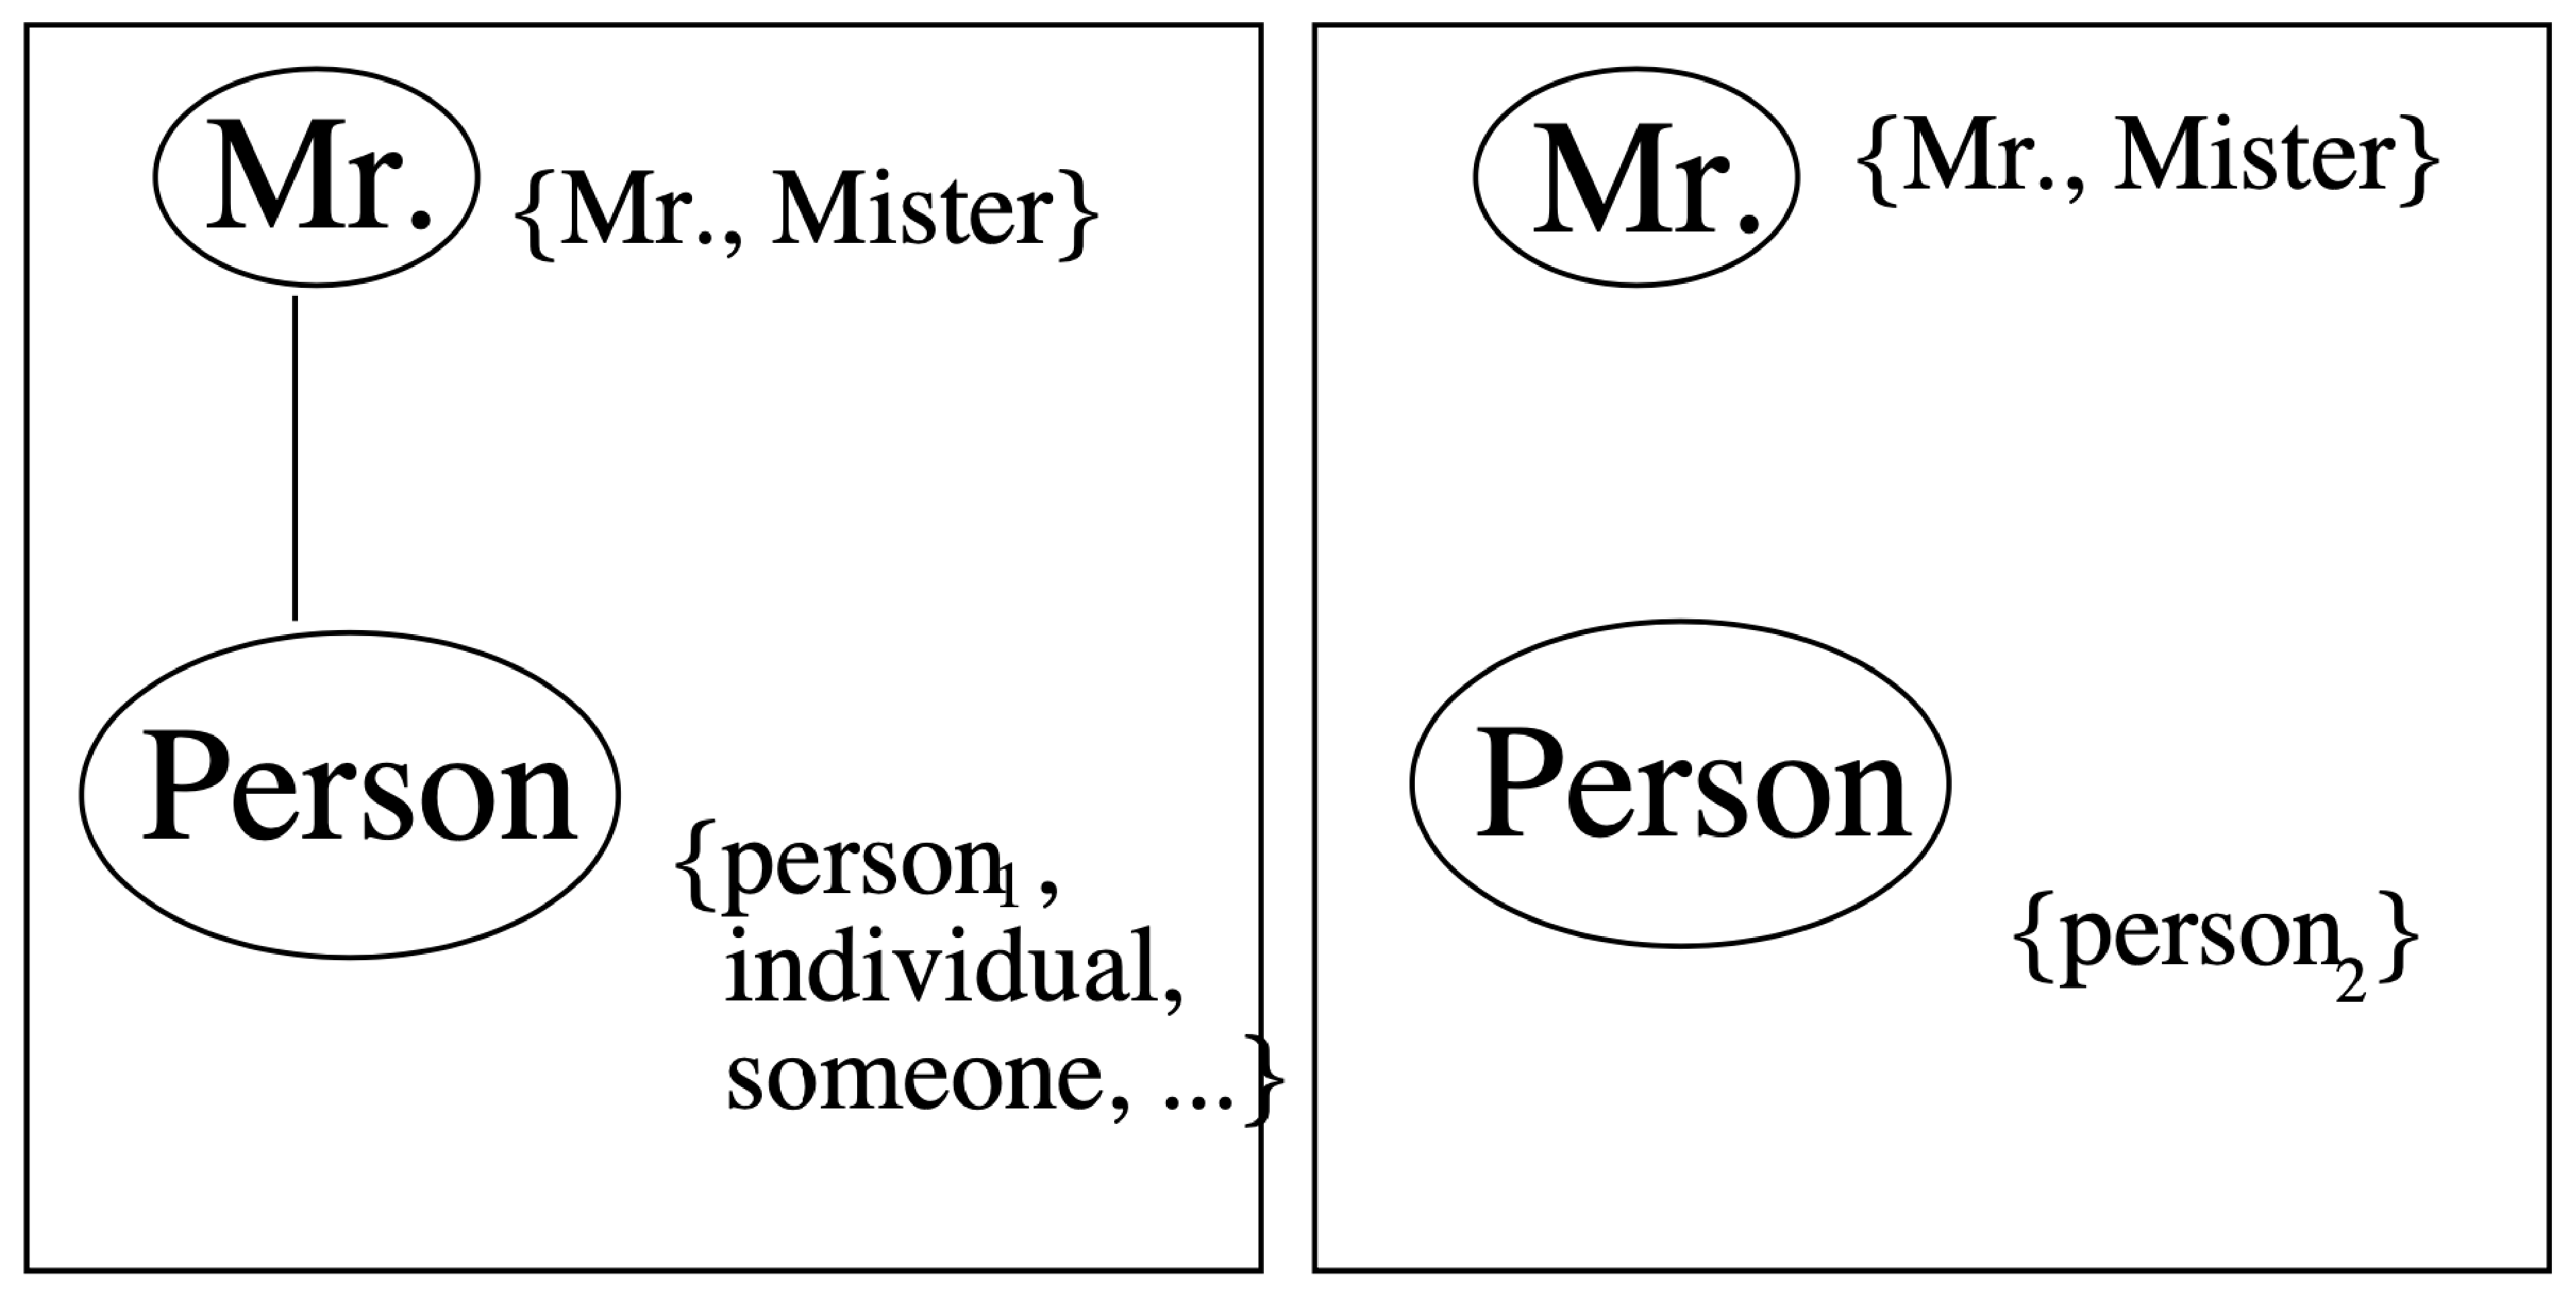
\includegraphics[width=\textwidth]{lexical_chains_step_1.eps}
\caption{Step 1, interpretations 1 and 2}
\end{subfigure}
\begin{subfigure}{0.35\textwidth}
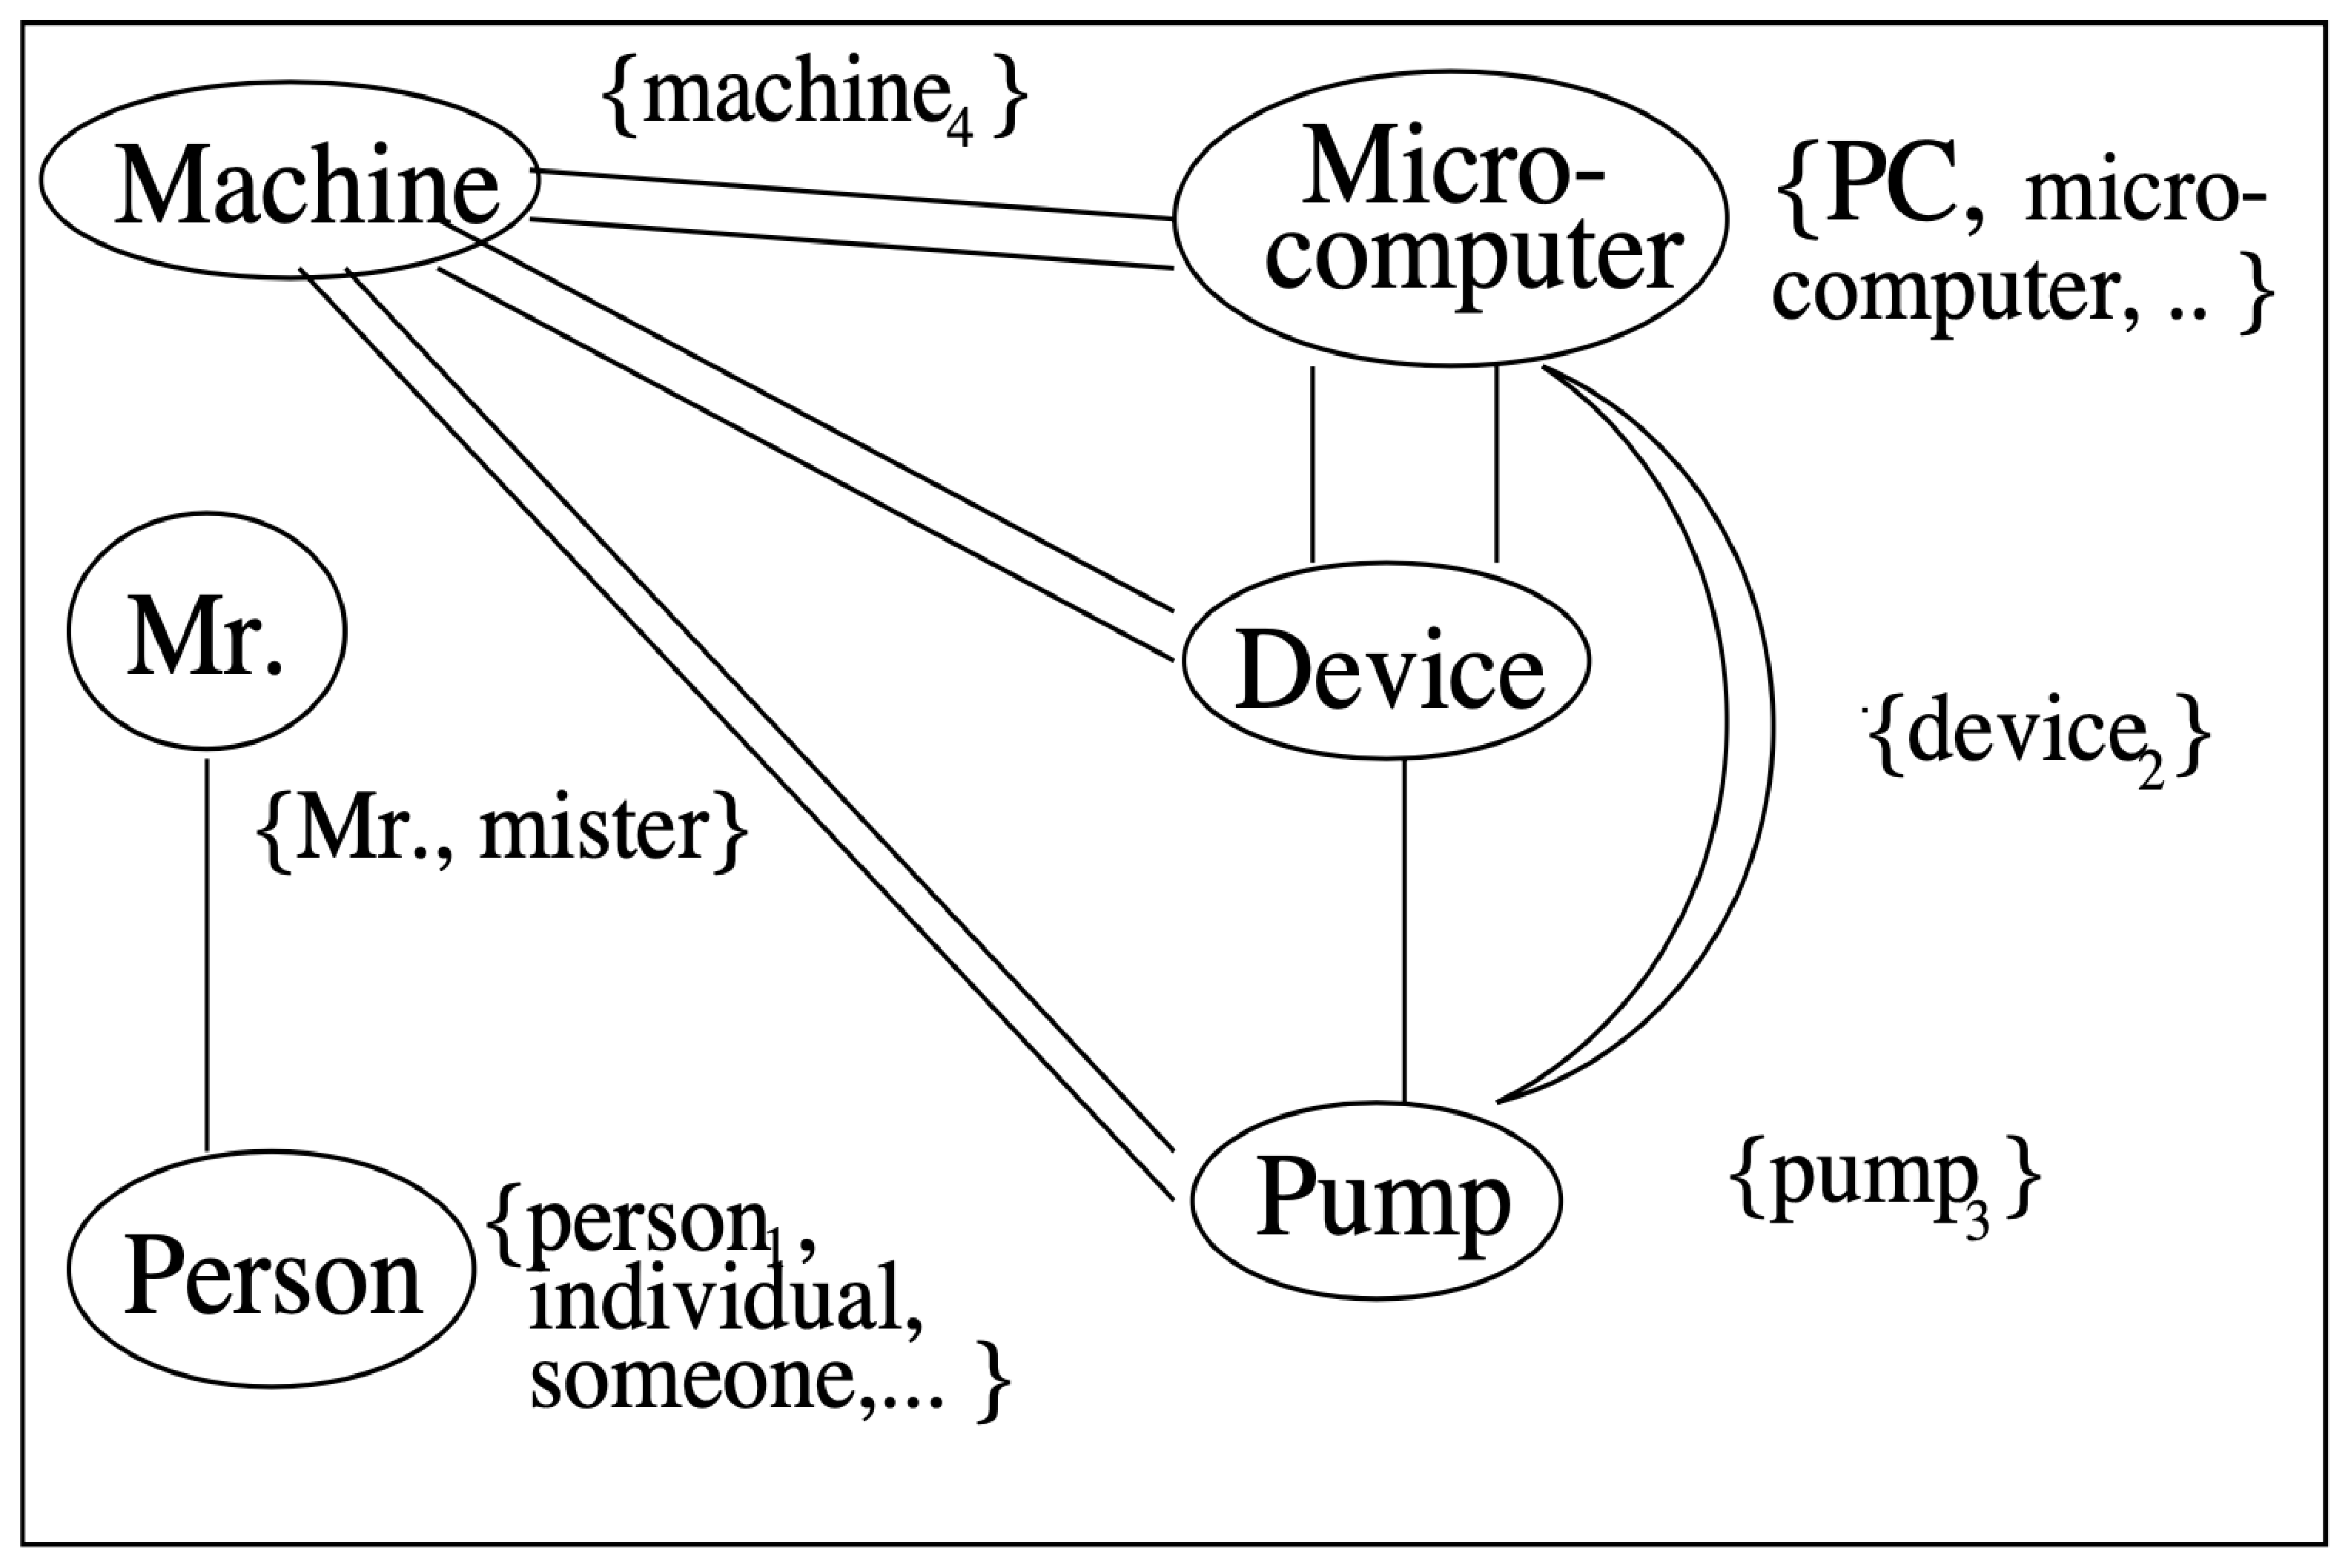
\includegraphics[width=\textwidth]{lexical_chains_step_3.eps}
\caption{Step 3, interpretation 1}
\end{subfigure}
\caption{\cite{barzilay_using_1997} Example of a \textit{lexical chain} and its interpretations}
\label{fig:lexical_chain_example}
\end{figure}

In order to construct the summary, a single ``important" sentence is extracted from the original text. To this end, they use a heuristic which is based on the fact that an important topic will discussed across the entire passage. Once a \textit{lexical chain} has been chosen according to this metric (i.e., one that is well distributed across the text), the output of the algorithm is the sentence which has the highest number of words from the selected \textit{lexical chain}.

\mbox{}

Although the proposed solution is very interesting in that it tries to link important words, it does not do anything whatsoever to learn any of the actions which are described in a passage. This means it has no knowledge of chronology (problematic when we have an action causing a change of state, such as a someone acquiring a good), nor does it try to link subjects with objects or verbs (for instance in the phrase ``Mary has a pencil", it does not link Mary to the pencil).

Furthermore, the algorithm outputs a singe unchanged sentence from the original text; this is suboptimal when equally important information is conveyed across multiple sentences. In a solution to the problem of text summarization, we would hope that important facts or actions are given as a summary. For the approach discussed here, this would mean picking out \textit{chunks} of text from the original passage, and combining them in a suitable manner.

\section{Approach Categories}

\subsection{Statistical}

In the statistical approach, the methodology is to use probabilities in order to generate a summary that is both grammatically correct and conveys the important details of a text.

\mbox{}

The authors of the paper \cite{knight_statistics-based_2000} envision what they call a \textit{noisy-channel model}, which at the time of writing was limited to single sentence summarization. For the  model, assume that there was at some point a (shorter) summary string $s$ for the (longer) string $t$ to summarize, from which optional words were removed. The idea is that optional details were added to produce $t$, and we want to know with what probability $s$ contained this information given $t$. At this stage, there a three problems to solve:
\begin{enumerate}[noitemsep]
\item To obtain the \textit{source model}, we must assign a probability $P(s)$ to every string $s$, which tells us how likely it is that this is the summary. If we assign a lower $P(s)$ to less grammatically correct strings, then it helps ensure that our final summary is well-formed.
\item To obtain the \textit{channel model}, we now assign the probabilities $P(t \vert s)$ to every pair $\langle s, t \rangle$. This contributes to preserving important information, as we take into account the differences between $s$ and $t$ when computing the corresponding probability. In this case, we may want to assign a very low $P(t \vert s)$ when $s$ omits an important verb or negation (these are not optional to get the correct meaning), while this can sometimes be much higher if the only difference is the word ``that".
\item For a given string $t$ the goal is now to maximize $P(s \vert t)$ which, because of \href{https://www.investopedia.com/terms/b/bayes-theorem.asp}{Bayes' theorem}, is equivalent to maximizing $P(s) \cdot P(t \vert s)$.
\end{enumerate}

In practice, the implementation discussed in the paper uses \textit{parse trees} rather than whole strings. Also, they use machine learning techniques in order to train their summarizer.

To this end, they created what was referred to in the paper as a \textit{shared-forest} structure, allowing them to represent all compressions given an original text $t$; an example is shown in Figure \ref{fig:statistics_example}. Their system picks out high-scoring trees from the forest, and based on this score we can choose the best compression $s$ for $t$ (i.e., the summary $s$ which has the highest $P(s) \cdot P(t \vert s)$).

If the user wants a shorter or longer summary, the system can simply return the highest-scoring tree for a given length. In reality though their solution is a bit more complex, but the important points of the approach are here.

\begin{figure}[H]
\begin{subfigure}{0.3\textwidth}
\quad \\
\quad \\
\phantom{\qquad}A $\rightarrow$ B C D \\
\phantom{\qquad}A $\rightarrow$ B C \\
\phantom{\qquad}A $\rightarrow$ C D \\
\phantom{\qquad}A $\rightarrow$ B D \\
\phantom{\qquad}A $\rightarrow$ B \\
\phantom{\qquad}D $\rightarrow$ E F \\
\phantom{\qquad}D $\rightarrow$ E \\
\phantom{\qquad}D $\rightarrow$ F \\
\caption{\textit{Shared-forest} structure}
\end{subfigure}
\begin{subfigure}{0.4\textwidth}
\centering
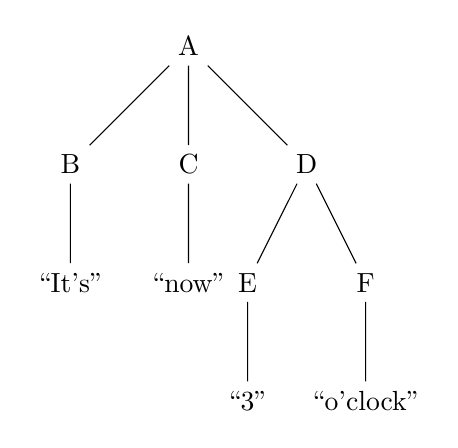
\begin{tikzpicture}
\node {A}
  child {node {B}
    child {node {``It's"}}}
  child {node {C}
    child {node {``now"}}}
  child {node {D}
    child {node {E}
      child {node {``3"}}}
    child {node {F}
      child {node {``o'clock"}}}};
\end{tikzpicture}
\caption{\textit{Parse tree} for $t$}
\end{subfigure}
\begin{subfigure}{0.25\textwidth}
\centering
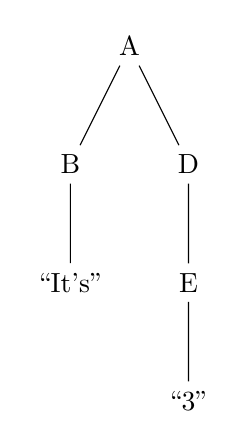
\begin{tikzpicture}
\node {A}
  child {node {B}
    child {node {``It's"}}}
  child {node {D}
    child {node {E}
      child {node {``3"}}}};
\end{tikzpicture}
\caption{\textit{Parse tree} for $s$}
\end{subfigure}
\caption{Example of an original text $t$ and possible summarization $s$}
\label{fig:statistics_example}
\end{figure}

In their testing it was found that their algorithm has a conservative nature, promoting correctness over brevity, which sometimes has the consequence of not trimming any words away. Therefore, this implementation is highly unsuitable for our purposes, but we shall nonetheless keep in mind the notion of the \textit{shared-forest} structure, as well as the use of Bayesian probability theory.

%In the decision-based model, they apply a sequence of shift-reduce-drop operations on the original sentence's parse tree \textit{t} in order to obtain the compressed sentence \textit{s} in the form of a stack. Starting from an empty stack, they are able to get a summary that can have a different ordering of words, which is not possible using the \textit{noisy-channel model}.

%After training these models using a set of newspaper articles with abstracts, they found that both were significantly better than the baseline they were using, although performed worse than humans. When run on a different dataset, they found that the decision-based model produced sentences that were more grammatically correct, however they would often be slightly over-compressed.

\subsection{Frame}

In the frame approach, the idea is that we try and keep track of how the plot in a story progresses, recording each action as well as the links which connect them. From this understanding, we should then have enough information to build an accurate summary.

\mbox{}

In one of the original papers describing this approach \cite{lehnert_1980_nodate}, sentences are decomposed into different \textit{affect states} and \textit{affect links}. An \textit{affect state} can either be a \textit{mental state}, or a \textit{positive} or \textit{negative event} which may cause a change to a \textit{mental state}. \textit{Affect links} are then the transitions that explain the sequence of \textit{affect states}.

We are given the example of John and Mary who both want to buy the same house, but it ends up being sold to Mary. At the start, both characters have the same \textit{mental state} (desire to buy the house). However the \textit{actualization} (a type of \textit{affect link} which denotes realization of an action) of Mary's desire is recognized as a \textit{positive event} for Mary and a \textit{negative event} for John.

By combining sequences of \textit{affect links} (transitions) between \textit{affect states} for different characters in a story, it is easy to see how one can build the narrative of the entire text. Such an example is shown in Figure \ref{fig:frame_example}, where \textit{m} denotes the \textit{motivation affect link} (connecting an action with a \textit{mental state} which it motivates), and \textit{e} denotes the \textit{equivalence affect link} (i.e., when a character has the same \textit{mental state} before and after the transition).

\begin{figure}[H]
\centering
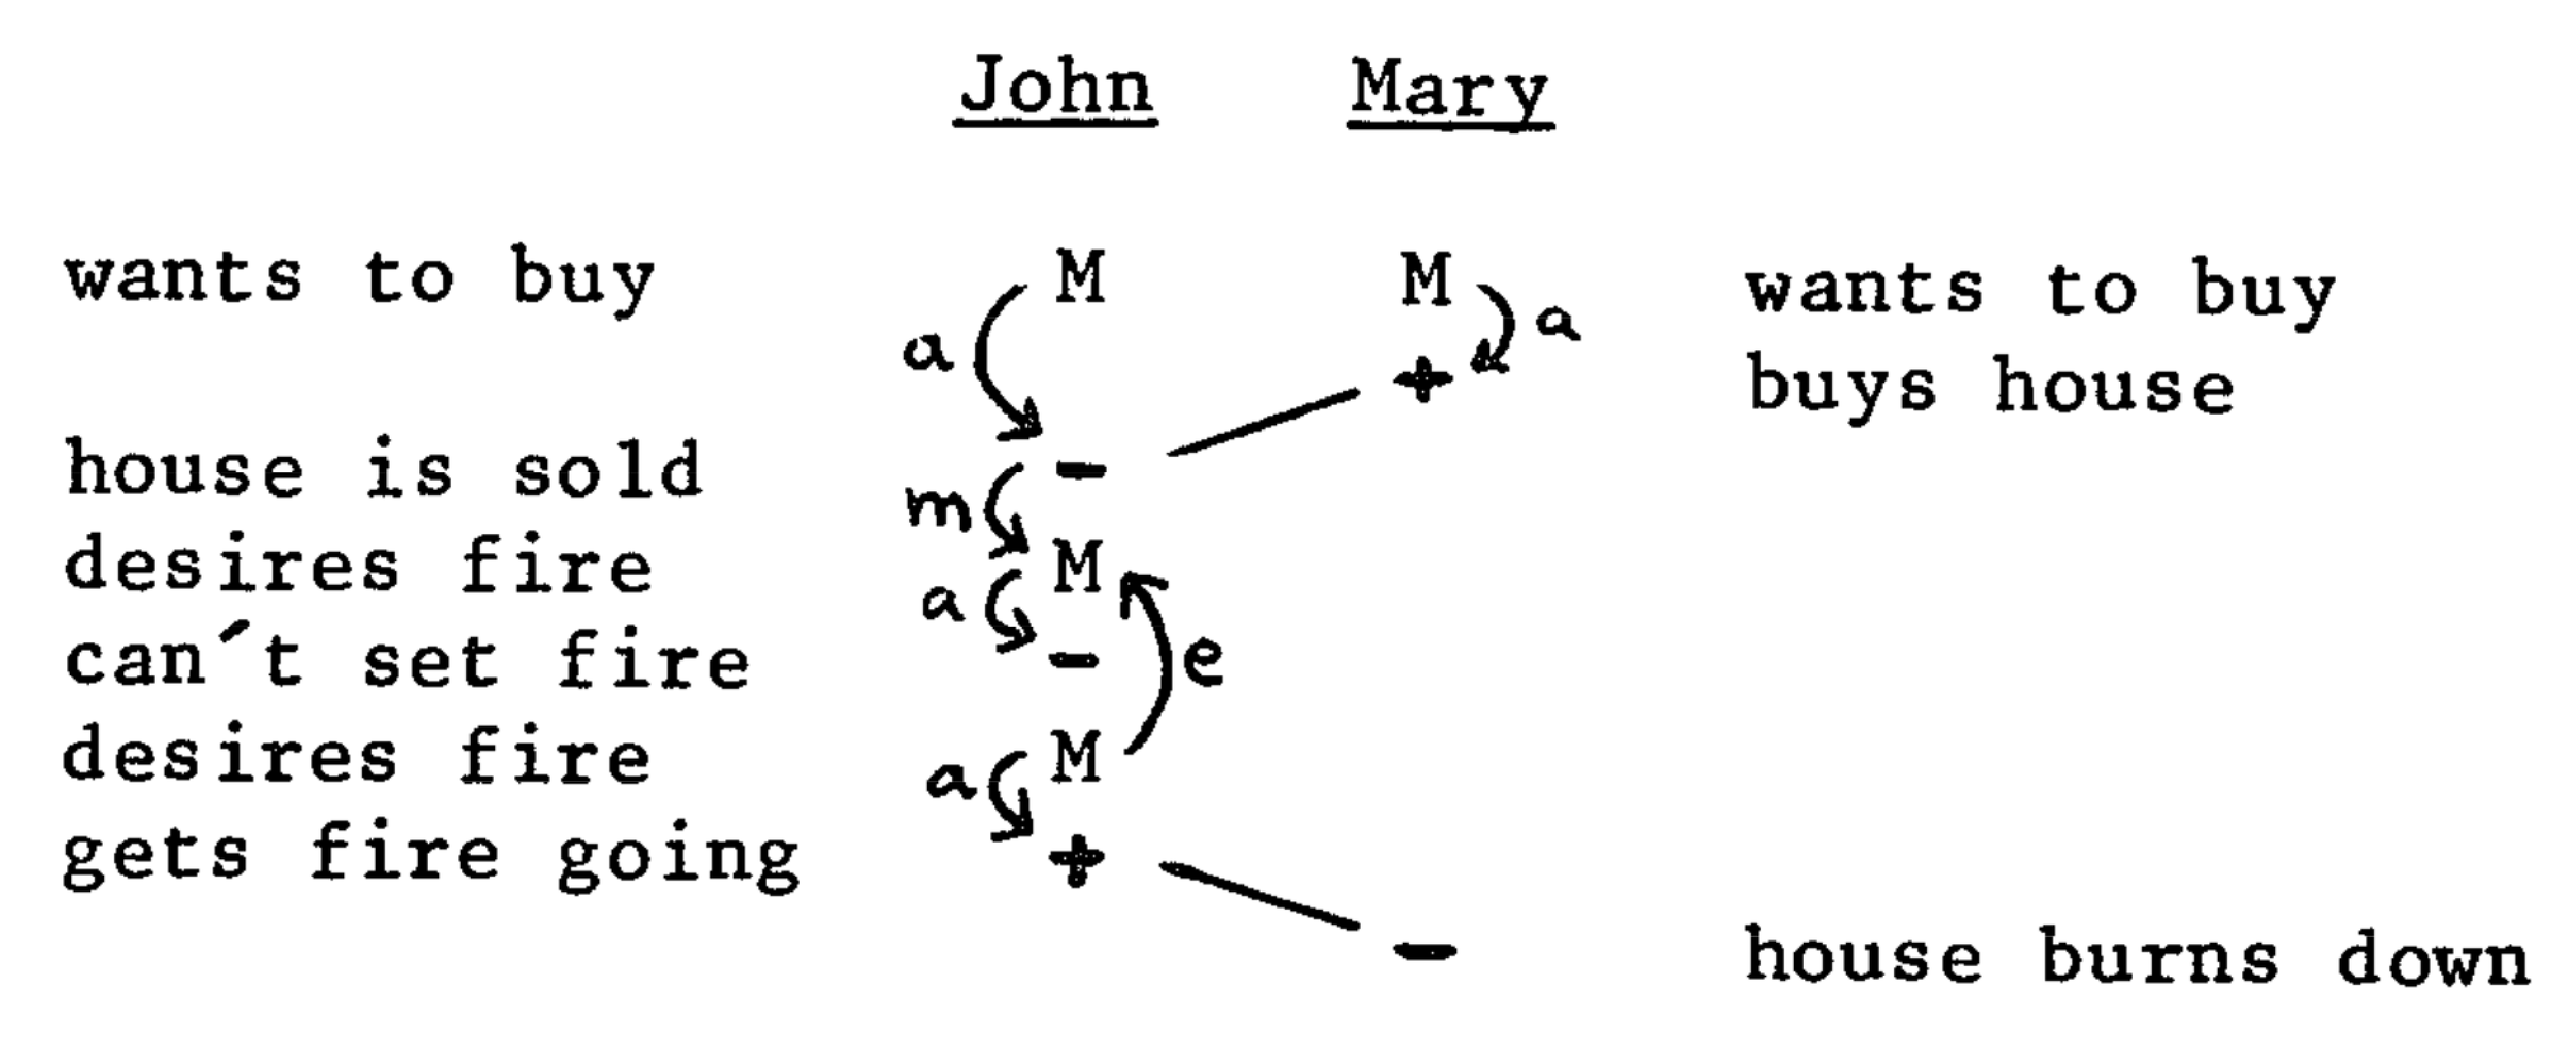
\includegraphics[width=0.7\textwidth]{frame_example.eps}
\caption{Example of a narrative in the frame approach}
\label{fig:frame_example}
\end{figure}

While this approach is interesting from a semantic point of view, it can easily become very complicated when many sentences are involved. In addition, it would not be suitable for purely descriptive texts, involving only continuous actions without any direct link (``It was October. Leaves were falling from the trees.").

\subsection{Symbolic}

In the symbolic approach \cite{clark_combining_nodate}, meaning is expressed through logic, and the representation of a sentence is the combination of the meaning of each of its individual components. CCG, as discussed in Subsection \ref{ssec:ccg}, uses a symbolic approach.

Generally the semantics of a word is captured as a single predicate in logic, and sometimes this is automatically derived from a large dataset such as an online dictionary. In order to obtain the final (sentential) logical form however, parsed sentences (represented for example as a \textit{parse tree}) must first be translated from their original (natural language) syntax. It then becomes possible to combine the meanings of words to obtain sentence fragments, and then combine these to understand the whole sentence. These can be further composed to cover an entire passage. This representation can then be provided to a theorem prover in \textit{first-order logic} (FOL), or directly converted into a logic program (for instance in ASP).

\mbox{}

Besides CCG, another pertinent case study is that of the Montague Grammar \cite{partee_lecture_nodate}. In such a grammar, we have what is called a \textit{syntactic language} and a \textit{semantic language}. The former is similar to POS tags (see Appendix \ref{appendix:pos}), while the latter captures the type of a token (which can either be $e$ for \textit{entity} or $t$ for \textit{truth value}). For instance, the word ``John" has \textit{syntactic category} ProperN and \textit{semantic type} $e$, while for the verb ``walks" these are respectively VP and $e \to t$.

For both of these languages, there exist rules that dictate how we are allowed to compose tokens. In the \textit{syntactic} case, this is simply a restriction on the format of \textit{parse trees} (i.e., $S \to NP\ VP$ means that a sentence node must have an NP and a VP as its children to be grammatically correct). For the \textit{semantic language}, combining tokens with respective types $A \to B$ and $A$ results in one whose type is $B$. Taking the example from before, ``John walks" would have type $t$; this makes sense because ``John" is an entity, and whether he is walking can either be true or false.

As we have seen above, these rules allow us to compose tokens together, and in the Montague Grammar everything has a logical representation (expressed in the $\lambda$-calculus). For instance, we would compose $\lambda P.[P(john)]$ with $walk$ to obtain $\lambda P.[P(john)](walk) \equiv walk(john)$. A more advanced example would be that ``every student walks" is represented as $\forall x.(student(x) \to walk(x))$.

\mbox{}

One of the criticisms with this approach \cite{clark_combining_nodate} is that it is domain-specific and not easily scalable. However more recent work (as with CCG) has shown that the latter issue is not necessarily the case any more, as we now have more powerful parsers. Should we choose to follow a symbolic approach, we shall hope to prove the former issue no longer relevant, once we have moved up from simpler examples.

%\section{General Method}

%In almost all these papers, the first step is to generate a parse tree in order to identify the different parts of speech and get a better understanding of a text. Once a parse tree is obtained, the task becomes to find out which details are important, and which can be omitted from the summary. Finally, the summary must be grammatically correct and provide enough information such that it serves a purpose to the reader.
%
%To know what is important...

\chapter{Conclusion}
\section{Achievements}

\textsc{SumASG*} is a symbolic system which is able to generate \textit{generic}, \textit{informative} and partially-\textit{abstractive} summaries given a simple story about a paragraph in length.

Internally, it relies on the ASG engine, which is used for both for understanding text and creating summary sentences. This is an \textit{entity level} approach to the task of text summarization, whereby the \textsc{Preprocessor} makes use of the \textit{similarity} between words and sentences, and creates a \textit{text relationship map} to aid in simplifying the given input story.

The core accomplishments of this project are the following:

\begin{itemize}
\item Created a context-free grammar that models the structure of basic English sentences, and can be used both for semantic learning, as well as generating grammatically-correct text.
\item Implemented an algorithm that dramatically reduces the complexity in the structure of English sentences, without losing too much information.
\item Implemented an algorithm which uses \textit{similarity} to remove irrelevant sentences from a short story.
\item Implemented a scoring mechanism prioritizing information density, while taking into account words which may appear frequently in English, can be considered as the \textit{topic} of the original text.
\item Created a framework to automatically generate topical short stories for evaluating the system, based on a dataset of words and a particular sentence structure.
\end{itemize}

\section{Future Work}

\textcolor{red}{\textbf{\hl{TODO}}}

- domain-specific, not scalable
- longer text
- more complex structure
- better verification methods
- better understanding of connectors and chronology
- more efficient

\begin{appendices}
\titleformat{\chapter}{\normalfont\huge}{\appendixname{} \thechapter.}{20pt}{\bfseries\huge}
\chapter{POS Tags}
\label{appendix:pos}

\begin{table}[H]
\centering
\begin{tabular}{@{}ll@{}}
\toprule
Tag & Description \\ \midrule
CC & Coordinating conjunction \\
CD & Cardinal number \\
DT & Determiner \\
EX & Existential there \\
FW & Foreign word \\
IN & Preposition or subordinating conjunction \\
JJ & Adjective \\
JJR & Adjective, comparative \\
JJS & Adjective, superlative \\
LS & List item marker \\
MD & Modal \\
NN & Noun, singular or mass \\
NNS & Noun, plural \\
NNP & Proper noun, singular \\
NNPS & Proper noun, plural \\
PDT & Predeterminer \\
POS & Possessive ending \\
PRP & Personal pronoun \\
PRP\$ & Possessive pronoun \\
RB & Adverb \\
RBR & Adverb, comparative \\
RBS & Adverb, superlative \\
RP & Particle \\
SYM & Symbol \\
TO & to \\
UH & Interjection \\
VB & Verb, base form \\
VBD & Verb, past tense \\
VBG & Verb, gerund or present participle \\
VBN & Verb, past participle \\
VBP & Verb, non-3rd person singular present \\
VBZ & Verb, 3rd person singular present \\
WDT & Wh-determiner \\
WP & Wh-pronoun \\
WP\$ & Possessive wh-pronoun \\
WRB & Wh-adverb \\ \bottomrule
\end{tabular}
\caption{\cite{noauthor_penn_nodate} List of position of speech (POS) tags}
\end{table}

\chapter{ASG}

\textcolor{red}{\textbf{\hl{TODO fix margin, separate task1 from task2 code}}}

\begin{lstlisting}
start -> s_group {
   :- count(X)@1, X > 1.
   :- count(X)@1, X = 0.
}

s_group -> {
  count(0).
}

s_group -> s_group s ". " {
  count(X+1) :- count(X)@1.

  % Reject output summaries with duplicate sentences
  sentence(X,V,O,S) :- output(_,V,O,S)@2, count(X).
  sentence(X,V,O,S) :- sentence(X,V,O,S)@1.
  :- sentence(X1,V,O,S), sentence(X2,V,O,S), X1 != X2.
}

s -> np vp {
  :- not action(verb(V_N,V_T),subject(S_N,S_D,S_A),object(O_N,O_D,O_A)), verb(V_N,V_T)@2, subject(S_N,S_D,S_A)@1, object(O_N,O_D,O_A)@2.

  subject :- subject(S_N,S_D,S_A)@1.
  :- not subject.
  object :- object(S_N,S_D,S_A)@2.
  :- not object.
}

vp -> vbn np {
  verb(N,T) :- verb(N,T)@1.
  object(N,D,A) :- object(N,D,A)@2.
}

vp -> vbd np {
  verb(N,T) :- verb(N,T)@1.
  object(N,D,A) :- object(N,D,A)@2.
}

vp -> vbd vbg np {
  verb(comp(N1,N2),comp(T1,gerund)) :- verb(N1,T1)@1, verb(N2,gerund)@2.
  object(N,D,A) :- object(N,D,A)@3.
}

vp -> vbd vbn np {
  verb(comp(N1,N2),comp(T1,past_part)) :- verb(N1,T1)@1, verb(N2,past_part)@2.
  object(N,D,A) :- object(N,D,A)@3.
}

vp -> vbd "to " vb np {
  verb(comp(N1,N2),comp(T1,base)) :- verb(N1,T1)@1, verb(N2,base)@3.
  object(N,D,A) :- object(N,D,A)@4.
}

vp -> vbp np {
  verb(N,T) :- verb(N,T)@1.
  object(N,D,A) :- object(N,D,A)@2.
}

vp -> vbp vbg np {
  verb(comp(N1,N2),comp(T1,gerund)) :- verb(N1,T1)@1, verb(N2,gerund)@2.
  object(N,D,A) :- object(N,D,A)@3.
}

vp -> vbp vbn np {
  verb(comp(N1,N2),comp(T1,past_part)) :- verb(N1,T1)@1, verb(N2,past_part)@2.
  object(N,D,A) :- object(N,D,A)@3.
}

vp -> vbp "to " vb np {
  verb(comp(N1,N2),comp(T1,base)) :- verb(N1,T1)@1, verb(N2,base)@3.
  object(N,D,A) :- object(N,D,A)@4.
}

vp -> vbz np {
  verb(N,T) :- verb(N,T)@1.
  object(N,D,A) :- object(N,D,A)@2.
}

vp -> vbz vbg np {
  verb(comp(N1,N2),comp(T1,gerund)) :- verb(N1,T1)@1, verb(N2,gerund)@2.
  object(N,D,A) :- object(N,D,A)@3.
}

vp -> vbz vbn np {
  verb(comp(N1,N2),comp(T1,past_part)) :- verb(N1,T1)@1, verb(N2,past_part)@2.
  object(N,D,A) :- object(N,D,A)@3.
}

vp -> vbz "to " vb np {
  verb(comp(N1,N2),comp(T1,base)) :- verb(N1,T1)@1, verb(N2,base)@3.
  object(N,D,A) :- object(N,D,A)@4.
}

np -> np rb {
  object(N,D,A) :- object(N,D,0)@1, adj_or_adv(A)@2.
}

np -> np rb {
  object(N,D,conjunct(A1,A2)) :- object(N,D,A1)@1, adj_or_adv(A2)@2.
  :- object(N,D,conjunct(A,A)).
}

np -> np rp {
  object(N,D,A) :- object(N,D,0)@1, adj_or_adv(A)@2.
}

np -> np rp {
  object(N,D,conjunct(A1,A2)) :- object(N,D,A1)@1, adj_or_adv(A2)@2.
  :- object(N,D,conjunct(A,A)).
}

np -> nn {
  subject(N,0,0) :- noun(N)@1.
  object(N,0,0) :- noun(N)@1.
}

np -> nns {
  subject(N,0,0) :- noun(N)@1.
  object(N,0,0) :- noun(N)@1.
}

np -> nnp {
  subject(N,0,0) :- noun(N)@1.
  object(N,0,0) :- noun(N)@1.
}

np -> nnps {
  subject(N,0,0) :- noun(N)@1.
  object(N,0,0) :- noun(N)@1.
}

np -> prp {
  subject(N,0,0) :- noun(N)@1.
  object(N,0,0) :- noun(N)@1.
}

np -> rb {
  subject(0,0,A) :- adj_or_adv(A)@1.
  object(0,0,A) :- adj_or_adv(A)@1.
}

np -> rp {
  subject(0,0,A) :- adj_or_adv(A)@1.
  object(0,0,A) :- adj_or_adv(A)@1.
}

np -> ex {
  subject(N,0,0) :- noun(N)@1.
}

np -> in {
  object(0,D,0) :- det(D)@1.
}

np -> prp "and " nnp {
  subject(conjunct(N1,N2),0,0) :- noun(N1)@1, noun(N2)@3.
  object(conjunct(N1,N2),0,0) :- noun(N1)@1, noun(N2)@3.
  :- subject(conjunct(N,N),0,0).
  :- object(conjunct(N,N),0,0).
}

np -> nnp "and " prp {
  subject(conjunct(N1,N2),0,0) :- noun(N1)@1, noun(N2)@3.
  object(conjunct(N1,N2),0,0) :- noun(N1)@1, noun(N2)@3.
  :- subject(conjunct(N,N),0,0).
  :- object(conjunct(N,N),0,0).
}

np -> dt nn "and " prp {
  subject(conjunct(N1,N2),D,0) :- det(D)@1, noun(N1)@2, noun(N2)@4.
  object(conjunct(N1,N2),D,0) :- det(D)@1, noun(N1)@2, noun(N2)@4.
  :- subject(conjunct(N,N),_,0).
  :- object(conjunct(N,N),_,0).
}

np -> prp "and " dt nn {
  subject(conjunct(N1,N2),D,0) :- noun(N1)@1, det(D)@3, noun(N2)@4.
  object(conjunct(N1,N2),D,0) :- noun(N1)@1, det(D)@3, noun(N2)@4.
  :- subject(conjunct(N,N),_,0).
  :- object(conjunct(N,N),_,0).
}

np -> dt nn "and " nnp {
  subject(conjunct(N1,N2),D,0) :- det(D)@1, noun(N1)@2, noun(N2)@4.
  object(conjunct(N1,N2),D,0) :- det(D)@1, noun(N1)@2, noun(N2)@4.
  :- subject(conjunct(N,N),_,0).
  :- object(conjunct(N,N),_,0).
}

np -> nnp "and " dt nn {
  subject(conjunct(N1,N2),D,0) :- noun(N1)@1, det(D)@3, noun(N2)@4.
  object(conjunct(N1,N2),D,0) :- noun(N1)@1, det(D)@3, noun(N2)@4.
  :- subject(conjunct(N,N),_,0).
  :- object(conjunct(N,N),_,0).
}

np -> nnp "and " nnp {
  subject(conjunct(N1,N2),0,0) :- noun(N1)@1, noun(N2)@3.
  object(conjunct(N1,N2),0,0) :- noun(N1)@1, noun(N2)@3.
  :- subject(conjunct(N,N),0,0).
  :- object(conjunct(N,N),0,0).
}

np -> nn "and " nn {
  subject(conjunct(N1,N2),0,0) :- noun(N1)@1, noun(N2)@3.
  object(conjunct(N1,N2),0,0) :- noun(N1)@1, noun(N2)@3.
  :- subject(conjunct(N,N),0,0).
  :- object(conjunct(N,N),0,0).
}

np -> nn "and " nns {
  subject(conjunct(N1,N2),0,0) :- noun(N1)@1, noun(N2)@3.
  object(conjunct(N1,N2),0,0) :- noun(N1)@1, noun(N2)@3.
  :- subject(conjunct(N,N),0,0).
  :- object(conjunct(N,N),0,0).
}

np -> nns "and " nn {
  subject(conjunct(N1,N2),0,0) :- noun(N1)@1, noun(N2)@3.
  object(conjunct(N1,N2),0,0) :- noun(N1)@1, noun(N2)@3.
  :- subject(conjunct(N,N),0,0).
  :- object(conjunct(N,N),0,0).
}

np -> nns "and " nns {
  subject(conjunct(N1,N2),0,0) :- noun(N1)@1, noun(N2)@3.
  object(conjunct(N1,N2),0,0) :- noun(N1)@1, noun(N2)@3.
  :- subject(conjunct(N,N),0,0).
  :- object(conjunct(N,N),0,0).
}

np -> prp "and " prp {
  subject(conjunct(N1,N2),0,0) :- noun(N1)@1, noun(N2)@3.
  object(conjunct(N1,N2),0,0) :- noun(N1)@1, noun(N2)@3.
  :- subject(conjunct(N,N),0,0).
  :- object(conjunct(N,N),0,0).
}

np -> rb "and " rb {
  subject(0,0,conjunct(A1,A2)) :- adj_or_adv(A1)@1, adj_or_adv(A2)@3.
  object(0,0,conjunct(A1,A2)) :- adj_or_adv(A1)@1, adj_or_adv(A2)@3.
  :- subject(0,0,conjunct(A,A)).
  :- object(0,0,conjunct(A,A)).
}

np -> jj {
  object(0,0,A) :- adj_or_adv(A)@1.
}

np -> jj "and " jj {
  object(0,0,conjunct(A1,A2)) :- adj_or_adv(A1)@1, adj_or_adv(A2)@3.
  :- object(0,0,conjunct(A,A)).
}

np -> jj rb {
  subject(0,0,conjunct(A1,A2)) :- adj_or_adv(A1)@1, adj_or_adv(A2)@1.
  object(0,0,conjunct(A1,A2)) :- adj_or_adv(A1)@1, adj_or_adv(A2)@1.
  :- subject(0,0,conjunct(A,A)).
  :- object(0,0,conjunct(A,A)).
}

np -> dt nn {
  subject(N,D,0) :- det(D)@1, noun(N)@2.
  object(N,D,0) :- det(D)@1, noun(N)@2.
}

np -> dt nns {
  subject(N,D,0) :- det(D)@1, noun(N)@2.
  object(N,D,0) :- det(D)@1, noun(N)@2.
}

np -> jj nns {
  subject(N,0,A) :- adj_or_adv(A)@1, noun(N)@2.
  object(N,0,A) :- adj_or_adv(A)@1, noun(N)@2.
}

np -> jj nnp {
  subject(N,0,A) :- adj_or_adv(A)@1, noun(N)@2.
  object(N,0,A) :- adj_or_adv(A)@1, noun(N)@2.
}

np -> jj nnps {
  subject(N,0,A) :- adj_or_adv(A)@1, noun(N)@2.
  object(N,0,A) :- adj_or_adv(A)@1, noun(N)@2.
}

np -> dt jj nn {
  subject(N,D,A) :- det(D)@1, adj_or_adv(A)@2, noun(N)@3.
  object(N,D,A) :- det(D)@1, adj_or_adv(A)@2, noun(N)@3.
}

np -> dt jj nns {
  subject(N,D,A) :- det(D)@1, adj_or_adv(A)@2, noun(N)@3.
  object(N,D,A) :- det(D)@1, adj_or_adv(A)@2, noun(N)@3.
}

np -> dt jj jj nn {
  subject(N,D,conjunct(A1,A2)) :- det(D)@1, adj_or_adv(A1)@2, adj_or_adv(A2)@3, noun(N)@4.
  object(N,D,conjunct(A1,A2)) :- det(D)@1, adj_or_adv(A1)@2, adj_or_adv(A2)@3, noun(N)@4.
  :- subject(N,D,conjunct(A,A)).
  :- object(N,D,conjunct(A,A)).
}

np -> dt jj jj nns {
  subject(N,D,conjunct(A1,A2)) :- det(D)@1, adj_or_adv(A1)@2, adj_or_adv(A2)@3, noun(N)@4.
  object(N,D,conjunct(A1,A2)) :- det(D)@1, adj_or_adv(A1)@2, adj_or_adv(A2)@3, noun(N)@4.
  :- subject(N,D,conjunct(A,A)).
  :- object(N,D,conjunct(A,A)).
}

np -> dt jjr nn {
  subject(N,D,A) :- det(D)@1, adj_or_adv(A)@2, noun(N)@3.
  object(N,D,A) :- det(D)@1, adj_or_adv(A)@2, noun(N)@3.
}

np -> dt jjr nns {
  subject(N,D,A) :- det(D)@1, adj_or_adv(A)@2, noun(N)@3.
  object(N,D,A) :- det(D)@1, adj_or_adv(A)@2, noun(N)@3.
}

np -> dt jjs nn {
  subject(N,D,A) :- det(D)@1, adj_or_adv(A)@2, noun(N)@3.
  object(N,D,A) :- det(D)@1, adj_or_adv(A)@2, noun(N)@3.
}

np -> dt jjs nns {
  subject(N,D,A) :- det(D)@1, adj_or_adv(A)@2, noun(N)@3.
  object(N,D,A) :- det(D)@1, adj_or_adv(A)@2, noun(N)@3.
}

np -> in nn {
  object(N,D,0) :- det(D)@1, noun(N)@2.
}

np -> in dt nn {
  object(N,conjunct(D1,D2),0) :- det(D1)@1, det(D2)@2, noun(N)@3.
}

np -> in nns {
  object(N,D,0) :- det(D)@1, noun(N)@2.
}

np -> in dt nns {
  object(N,conjunct(D1,D2),0) :- det(D1)@1, det(D2)@2, noun(N)@3.
}

np -> in nnp {
  object(N,D,0) :- det(D)@1, noun(N)@2.
}

np -> in nnps {
  object(N,D,0) :- det(D)@1, noun(N)@2.
}

np -> jj in nn {
  object(N,D,A) :- adj_or_adv(A)@1, det(D)@2, noun(N)@3.
}

np -> jj in nn "and " nn {
  object(conjunct(N1,N2),D,A) :- adj_or_adv(A)@1, det(D)@2, noun(N1)@3, noun(N2)@5.
}

np -> jj in nns {
  object(N,D,A) :- adj_or_adv(A)@1, det(D)@2, noun(N)@3.
}

np -> jj in nns "and " nns {
  object(conjunct(N1,N2),D,A) :- adj_or_adv(A)@1, det(D)@2, noun(N1)@3, noun(N2)@5.
}

np -> jj in nnp {
  object(N,D,A) :- adj_or_adv(A)@1, det(D)@2, noun(N)@3.
}

np -> jj in nnp "and " nnp {
  object(conjunct(N1,N2),D,A) :- adj_or_adv(A)@1, det(D)@2, noun(N1)@3, noun(N2)@5.
}

np -> jj in prp {
  object(N,D,A) :- adj_or_adv(A)@1, det(D)@2, noun(N)@3.
}

np -> jj in prp "and " prp {
  object(conjunct(N1,N2),D,A) :- adj_or_adv(A)@1, det(D)@2, noun(N1)@3, noun(N2)@5.
}

np -> jj in nn "and " nns {
  object(conjunct(N1,N2),D,A) :- adj_or_adv(A)@1, det(D)@2, noun(N1)@3, noun(N2)@5.
}

np -> jj in nns "and " nn {
  object(conjunct(N1,N2),D,A) :- adj_or_adv(A)@1, det(D)@2, noun(N1)@3, noun(N2)@5.
}

np -> cd nn {
  subject(N,D,0) :- det(D)@1, noun(N)@2.
  object(N,D,0) :- det(D)@1, noun(N)@2.
}

np -> cd nns {
  subject(N,D,0) :- det(D)@1, noun(N)@2.
  object(N,D,0) :- det(D)@1, noun(N)@2.
}

np -> cd jj nn {
  subject(N,D,A) :- det(D)@1, adj_or_adv(A)@2, noun(N)@3.
  object(N,D,A) :- det(D)@1, adj_or_adv(A)@2, noun(N)@3.
}

np -> cd jj nns {
  subject(N,D,A) :- det(D)@1, adj_or_adv(A)@2, noun(N)@3.
  object(N,D,A) :- det(D)@1, adj_or_adv(A)@2, noun(N)@3.
}

np -> cd nns jj {
  object(N,D,A) :- det(D)@1, noun(N)@2, adj_or_adv(A)@3.
}

np -> dt jj cd {
  subject(0,conjunct(D1,D2),A) :- det(D1)@1, adj_or_adv(A)@2, det(D2)@3.
  object(0,conjunct(D1,D2),A) :- det(D1)@1, adj_or_adv(A)@2, det(D2)@3.
}


\end{lstlisting}
\end{appendices}

%\nocite{*}
\bibliographystyle{vancouver}
\bibliography{references}
\pagestyle{PageNum}

\end{document}